% !TEX encoding   = UTF8
% !TEX spellcheck = ru_RU

\documentclass[a4paper,12pt,oneside,openany,final]{memoir}

% !TEX encoding   = UTF8
% !TEX spellcheck = en_US


%%% Page layout %%%
\usepackage{pdflscape}
\usepackage{geometry}

%%% Mathematics %%%
\usepackage{amsthm,amsfonts,amsmath,amscd}
\usepackage{mathtools}             % Add environment 'multlined'
\usepackage{dsfont}
\usepackage{unicode-math}

%%% Encodings and fonts %%%
\usepackage{polyglossia}[2014/05/21]  % Automatically load 'fontspec'

%%% Paragraph layout %%%
\usepackage{indentfirst}
\usepackage{epigraph}
\usepackage[style=french]{csquotes}

%%% Colors %%%
\usepackage[svgnames,table,hyperref]{xcolor} %,cmyk

%%% Tables %%%
\usepackage{longtable,ltcaption}
\usepackage{multirow,makecell}     % Advanced formatting
\usepackage{tabu,tabulary}         % Automatic columns width
\usepackage{array}
\usepackage{hhline}
\usepackage{multicol}

%%% General layout %%%
\usepackage{soulutf8}              % Underlying with hyphenation
\usepackage{icomma}
\usepackage{calc}
\usepackage[normalem]{ulem}

%%% Hyper references %%%
\usepackage{hyperref}

%%% Figures %%%
\usepackage{graphicx}
\usepackage{tikz}
\usetikzlibrary{arrows,decorations.pathmorphing,backgrounds,positioning,fit,calc}
\usetikzlibrary{arrows.meta}
\usetikzlibrary{shapes,shapes.misc}
\usetikzlibrary{graphs, graphdrawing}
\usegdlibrary{trees, layered}
\usepackage{wrapfig}

%%% Lists %%%
\usepackage[inline]{enumitem}

%%% Embedded languages %%%
\usepackage[usefamily={py,sympy},rerun=always]{pythontex}

%%% Listings %%%
\usepackage{verbatim}
\usepackage{minted}
\usepackage{listings}
\lccode`\~=0\relax                 % Fix \MakeLowercase etc. with (xe|lua)latex

%%% Smart references %%%
%\usepackage{cleveref}


% !TEX encoding   = UTF8
% !TEX spellcheck = en_EN

\usepackage{csquotes}
\usepackage[backend=biber,%
            bibencoding=utf8,%
            citestyle=gost-inline-min,%gost-numeric,%
            bibstyle=gost-numeric,%
            sorting=none,%
            defernumbers=true,%
            sortcites=true,%
            doi=false,%
            isbn=false,%
            autolang=langname]{biblatex}


\DeclareFieldFormat{url}{
  \mkbibacro{URL}\addcolon\space\href{#1}{\nolinkurl{\thefield{urlraw}}}
}


% !TEX encoding   = UTF8
% !TEX spellcheck = en_US


%%% Hyper references colors %%%

\definecolor{linkcolor}{rgb}{0.9,0,0}
\definecolor{citecolor}{rgb}{0,0.6,0}
\definecolor{urlcolor}{rgb}{0,0,1}



%%% Define names %%%

\newcommand*\paperOrganization{\todo{Organization}}
\newcommand*\paperOrganizationShort{\todo{OShort}}
\newcommand*\paperDepartment{\todo{Department}}
\newcommand*\paperDepartmentShort{\todo{DShort}}
\newcommand*\paperTitle{\todo{Title}}
\newcommand*\paperSubject{\todo{Subject}}
\newcommand*\paperAuthor{\todo{\textcopyright{}perto}}
\newcommand*\paperKeywords{\todo{Keywords}}
\newcommand*\paperDate{\todo{Date}}
\newcommand*\paperYear{\todo{Year}}

% !TEX encoding   = UTF8
% !TEX spellcheck = en_US


%%% Redefine names %%%

\renewcommand*\paperOrganization{Московский физико-технический институт \\
    (государственный университет)}
\renewcommand*\paperOrganizationShort{МФТИ}
\renewcommand*\paperDepartment{Факультет аэромеханики и летательной техники}
\renewcommand*\paperDepartmentShort{ФАЛТ}
\renewcommand*\paperTitle{Архитектура компьютера и язык ассемблера}
\renewcommand*\paperAuthor{\textcopyright Преподаватели}
\renewcommand*\paperKeywords{МФТИ, ФАЛТ, информатика, программирование, язык С++}
\renewcommand*\paperDate{\textit{2023--2024 уч.\,гг.}}
\renewcommand*\paperYear{2023--2024\,гг.}


\renewcommand*\paperSubject{\href{\latexurl}{\TeX}нические материалы семинаров}

% !TEX encoding   = UTF8
% !TEX spellcheck = en_US


%%% Template %%%

\DeclareRobustCommand{\todo}{\textcolor{red}}

\AtBeginDocument{%
  \setlength{\parindent}{2.5em}
}



%%% Encondings and fonts %%%

\setmainlanguage[babelshorthands=true]{russian}
\setotherlanguage{english}

\setmonofont{Source Code Pro}
\newfontfamily\cyrillicfonttt{Source Code Pro}

\defaultfontfeatures{Ligatures=TeX}  % NB! monofont settings should be before this

\setmainfont{STIX Two Text}
\newfontfamily\cyrillicfont{STIX Two Text}

\setsansfont{Source Sans 3}
\newfontfamily\cyrillicfontsf{Source Sans 3}

\setmathfont{STIX Two Math}
\newfontfamily\cyrillicfontmf{STIX Two Math}



%%% Captions %%%

\setlength{\abovecaptionskip}{0pt}
\setlength{\belowcaptionskip}{0pt}

\captionwidth{\linewidth}
\normalcaptionwidth



%%% Figures %%%

\setfloatadjustment{figure}{%
  \setlength{\abovecaptionskip}{0pt}
  \setlength{\belowcaptionskip}{0pt}
  \precaption{}
  \captionnamefont{\normalfont\normalsize}
  \captiondelim{~--- }
  \captionstyle[\centering]{\centering}
  \captiontitlefont{\normalfont\normalsize}
  \postcaption{}
}



%%% Subfigures captions %%%

\newsubfloat{figure}
\renewcommand{\thesubfigure}{\asbuk{subfigure}}
\subcaptionsize{\normalsize}
\subcaptionlabelfont{\normalfont}
\subcaptionfont{\!\!) \normalfont}  % round bracket after a letter
\subcaptionstyle{\centering}



%%% Tables %%%

\setfloatlocations{table}{!h}


%%% Hyper references settings %%%

\hypersetup{
  unicode,
  linktocpage=true,
%  linktoc=all,                % both the section and page part are links
%  pdfpagelabels=false,
  plainpages=false,
  colorlinks,
  linkcolor={linkcolor},
  citecolor={citecolor},
  urlcolor={urlcolor},
%  hidelinks,
  pdftitle={\paperTitle},
  pdfauthor={\paperAuthor},
  pdfsubject={\paperSubject},
  pdfkeywords={\paperKeywords},
  pdflang={ru},
}



%%% Lists %%%

\renewcommand{\labelitemi}{\normalfont\bfseries{--}}

%\renewcommand{\theenumi}{\alph{enumi}}
%\renewcommand{\labelenumi}{\theenumi)}

\makeatletter
\AddEnumerateCounter{\Asbuk}{\russian@Alph}{Щ}
\AddEnumerateCounter{\asbuk}{\russian@alph}{щ}
\makeatother

%\renewcommand{\theenumi}{\asbuk{enumi}}
%\renewcommand{\labelenumi}{\theenumi)}

\renewcommand{\theenumii}{\asbuk{enumii}}
\renewcommand{\labelenumii}{\theenumii)}

\renewcommand{\theenumiii}{\arabic{enumiii}}
\renewcommand{\labelenumiii}{\theenumiii)}

\setlist{%
  nosep,%
  labelindent=\parindent,leftmargin=*%
}

\newlist{enumIssue}{enumerate}{1}
\setlist[enumIssue]{label=\Asbuk*., ref=\Asbuk*}

\newlist{enumissue}{enumerate}{1}
\newlist{enumissue*}{enumerate*}{1}
\setlist[enumissue,enumissue*]{label=\textit{\asbuk*}), ref=\textit{\asbuk*}}

\newlist{itemfeature}{itemize}{1}
\setlist[itemfeature]{label=--, topsep=\medskipamount}



%%% Listings %%%

\usemintedstyle{manni}

\renewcommand{\theFancyVerbLine}{%
  \textcolor{gray}{\tiny\arabic{FancyVerbLine}}%
}

\newmintinline{c}{fontsize=\small}
\newmintinline{cpp}{fontsize=\small}
\newmintinline{gas}{fontsize=\small}
\newmintinline{text}{fontsize=\small}

\newmint[cc]{c}{fontsize=\small, escapeinside=||}
\newmint{cpp}{fontsize=\small}
\newmint{js}{fontsize=\small}
\newmint{gas}{fontsize=\small}
\newmint[txt]{text}{fontsize=\small}
\newmint{console}{fontsize=\small}
\newmint[precomment]{text}{fontsize=\footnotesize, formatcom=\color{cyan}}

\newminted{c}{linenos, fontsize=\small, numbersep=0.2em, escapeinside=||}
\newminted{cpp}{linenos, fontsize=\small, numbersep=0.2em}
\newminted{gas}{linenos, fontsize=\small, numbersep=0.2em, tabsize=2}
\newminted{text}{fontsize=\small, tabsize=2}
\newminted{console}{fontsize=\small, tabsize=2}

\newmintedfile{c}{linenos, fontsize=\small, numbersep=0.2em, stripnl}
\newmintedfile{cpp}{linenos, fontsize=\small, numbersep=0.2em}
\newmintedfile{js}{linenos, fontsize=\small, numbersep=0.2em}
\newmintedfile{gas}{linenos, fontsize=\small, numbersep=0.2em, tabsize=2}
\newmintedfile{objdump}{linenos, fontsize=\small, numbersep=0.2em, tabsize=2, escapeinside=||}
\newmintedfile{text}{fontsize=\small, tabsize=2}
\newmintedfile{console}{fontsize=\small, tabsize=2}


\newminted[precode]{text}{fontsize=\footnotesize, formatcom=\color{cyan}}



%%% General layout %%%

\DeclareRobustCommand*{\name}{\texttt}
\DeclareRobustCommand*{\code}[1]{\name{\small #1}}
\DeclareRobustCommand*{\codebf}[1]{\code{\bfseries #1}}
\DeclareRobustCommand*{\lang}[1]{\name{#1}}

\newcommand*{\comm}[1]{{\color{cyan}\ttfamily\footnotesize\itshape #1}}

\newcommand*{\styleans}[1]{\color{cyan}\underline{\color{gray!40}\ttfamily{}#1}}
\newcommand*{\showans}[1]{\phantom{#1}}
\newcommand*{\ansx}[1]{}
\newcommand*{\ansdots}[1]{\textcolor{cyan}{\ttfamily ...}}

\newcommand*{\ansfwnostar}[2]{\styleans{\makebox[#1][l]{\showans{#2}}}}
\newcommand*{\ansfwstar}[2]{\styleans{\makebox[#1][l]{\color{black}#2}}}
\newcommand*{\ansvwnostar}[1]{\styleans{\showans{#1}}}
\newcommand*{\ansvwstar}[1]{\styleans{\color{black}#1}}

\makeatletter
\newcommand*{\ansfw}{\@ifstar\ansfwstar\ansfwnostar}
\newcommand*{\ansvw}{\@ifstar\ansvwstar\ansvwnostar}
\makeatother

\newcommand*{\ArrowTo}[1]{%
  \tikz[baseline=#1]{
    \draw[white, -{Stealth[black, length=18pt, open]}] (0,0) -- (0.01,0)
  }%
}

\newcommand*{\mystyle}[1]{\textit{\ttfamily\footnotesize{}#1}}

% !TEX encoding   = UTF8
% !TEX spellcheck = en_US


%%% Template %%%

\DeclareRobustCommand{\todo}{\textcolor{red}}

\AtBeginDocument{%
  \setlength{\parindent}{2.5em}
}



%%% Encondings and fonts %%%

\setmainlanguage[babelshorthands=true]{russian}
\setotherlanguage{english}

\setmonofont{Source Code Pro}
\newfontfamily\cyrillicfonttt{Source Code Pro}

\defaultfontfeatures{Ligatures=TeX}  % NB! monofont settings should be before this

\setmainfont{STIX Two Text}
\newfontfamily\cyrillicfont{STIX Two Text}

\setsansfont{Source Sans 3}
\newfontfamily\cyrillicfontsf{Source Sans 3}

\setmathfont{STIX Two Math}
\newfontfamily\cyrillicfontmf{STIX Two Math}



%%% Captions %%%

\setlength{\abovecaptionskip}{0pt}
\setlength{\belowcaptionskip}{0pt}

\captionwidth{\linewidth}
\normalcaptionwidth



%%% Figures %%%

\setfloatadjustment{figure}{%
  \setlength{\abovecaptionskip}{0pt}
  \setlength{\belowcaptionskip}{0pt}
  \precaption{}
  \captionnamefont{\normalfont\normalsize}
  \captiondelim{~--- }
  \captionstyle[\centering]{\centering}
  \captiontitlefont{\normalfont\normalsize}
  \postcaption{}
}



%%% Subfigures captions %%%

\newsubfloat{figure}
\renewcommand{\thesubfigure}{\asbuk{subfigure}}
\subcaptionsize{\normalsize}
\subcaptionlabelfont{\normalfont}
\subcaptionfont{\!\!) \normalfont}  % round bracket after a letter
\subcaptionstyle{\centering}



%%% Tables %%%

\setfloatlocations{table}{!h}


%%% Hyper references settings %%%

\hypersetup{
  unicode,
  linktocpage=true,
%  linktoc=all,                % both the section and page part are links
%  pdfpagelabels=false,
  plainpages=false,
  colorlinks,
  linkcolor={linkcolor},
  citecolor={citecolor},
  urlcolor={urlcolor},
%  hidelinks,
  pdftitle={\paperTitle},
  pdfauthor={\paperAuthor},
  pdfsubject={\paperSubject},
  pdfkeywords={\paperKeywords},
  pdflang={ru},
}



%%% Lists %%%

\renewcommand{\labelitemi}{\normalfont\bfseries{--}}

%\renewcommand{\theenumi}{\alph{enumi}}
%\renewcommand{\labelenumi}{\theenumi)}

\makeatletter
\AddEnumerateCounter{\Asbuk}{\russian@Alph}{Щ}
\AddEnumerateCounter{\asbuk}{\russian@alph}{щ}
\makeatother

%\renewcommand{\theenumi}{\asbuk{enumi}}
%\renewcommand{\labelenumi}{\theenumi)}

\renewcommand{\theenumii}{\asbuk{enumii}}
\renewcommand{\labelenumii}{\theenumii)}

\renewcommand{\theenumiii}{\arabic{enumiii}}
\renewcommand{\labelenumiii}{\theenumiii)}

\setlist{%
  nosep,%
  labelindent=\parindent,leftmargin=*%
}

\newlist{enumIssue}{enumerate}{1}
\setlist[enumIssue]{label=\Asbuk*., ref=\Asbuk*}

\newlist{enumissue}{enumerate}{1}
\newlist{enumissue*}{enumerate*}{1}
\setlist[enumissue,enumissue*]{label=\textit{\asbuk*}), ref=\textit{\asbuk*}}

\newlist{itemfeature}{itemize}{1}
\setlist[itemfeature]{label=--, topsep=\medskipamount}



%%% Listings %%%

\usemintedstyle{manni}

\renewcommand{\theFancyVerbLine}{%
  \textcolor{gray}{\tiny\arabic{FancyVerbLine}}%
}

\newmintinline{c}{fontsize=\small}
\newmintinline{cpp}{fontsize=\small}
\newmintinline{gas}{fontsize=\small}
\newmintinline{text}{fontsize=\small}

\newmint[cc]{c}{fontsize=\small, escapeinside=||}
\newmint{cpp}{fontsize=\small}
\newmint{js}{fontsize=\small}
\newmint{gas}{fontsize=\small}
\newmint[txt]{text}{fontsize=\small}
\newmint{console}{fontsize=\small}
\newmint[precomment]{text}{fontsize=\footnotesize, formatcom=\color{cyan}}

\newminted{c}{linenos, fontsize=\small, numbersep=0.2em, escapeinside=||}
\newminted{cpp}{linenos, fontsize=\small, numbersep=0.2em}
\newminted{gas}{linenos, fontsize=\small, numbersep=0.2em, tabsize=2}
\newminted{text}{fontsize=\small, tabsize=2}
\newminted{console}{fontsize=\small, tabsize=2}

\newmintedfile{c}{linenos, fontsize=\small, numbersep=0.2em, stripnl}
\newmintedfile{cpp}{linenos, fontsize=\small, numbersep=0.2em}
\newmintedfile{js}{linenos, fontsize=\small, numbersep=0.2em}
\newmintedfile{gas}{linenos, fontsize=\small, numbersep=0.2em, tabsize=2}
\newmintedfile{objdump}{linenos, fontsize=\small, numbersep=0.2em, tabsize=2, escapeinside=||}
\newmintedfile{text}{fontsize=\small, tabsize=2}
\newmintedfile{console}{fontsize=\small, tabsize=2}


\newminted[precode]{text}{fontsize=\footnotesize, formatcom=\color{cyan}}



%%% General layout %%%

\DeclareRobustCommand*{\name}{\texttt}
\DeclareRobustCommand*{\code}[1]{\name{\small #1}}
\DeclareRobustCommand*{\codebf}[1]{\code{\bfseries #1}}
\DeclareRobustCommand*{\lang}[1]{\name{#1}}

\newcommand*{\comm}[1]{{\color{cyan}\ttfamily\footnotesize\itshape #1}}

\newcommand*{\styleans}[1]{\color{cyan}\underline{\color{gray!40}\ttfamily{}#1}}
\newcommand*{\showans}[1]{\phantom{#1}}
\newcommand*{\ansx}[1]{}
\newcommand*{\ansdots}[1]{\textcolor{cyan}{\ttfamily ...}}

\newcommand*{\ansfwnostar}[2]{\styleans{\makebox[#1][l]{\showans{#2}}}}
\newcommand*{\ansfwstar}[2]{\styleans{\makebox[#1][l]{\color{black}#2}}}
\newcommand*{\ansvwnostar}[1]{\styleans{\showans{#1}}}
\newcommand*{\ansvwstar}[1]{\styleans{\color{black}#1}}

\makeatletter
\newcommand*{\ansfw}{\@ifstar\ansfwstar\ansfwnostar}
\newcommand*{\ansvw}{\@ifstar\ansvwstar\ansvwnostar}
\makeatother

\newcommand*{\ArrowTo}[1]{%
  \tikz[baseline=#1]{
    \draw[white, -{Stealth[black, length=18pt, open]}] (0,0) -- (0.01,0)
  }%
}

\newcommand*{\mystyle}[1]{\textit{\ttfamily\footnotesize{}#1}}



\addbibresource{references.bib}




\begin{document}

% !TEX encoding   = UTF8
% !TEX spellcheck = ru_RU

\thispagestyle{empty}%
\begin{center}%
  \paperOrganization
\end{center}%
%
\vspace{0pt plus 6fill}%
%
\begin{center}
  
\includegraphics[width=15em]{images/falt_logo.jpg}
\end{center}
%
\vspace{0pt plus 4fill}%
%
\begin{center}%
\paperDepartment
\end{center}%
%
\vspace{0pt plus 1fill}%
%
\begin{center}%
\textbf{\Huge\paperTitle}

\vspace{0pt plus 2fill}%
\textit{\large \paperSubject}

\vspace{0pt plus 4fill}%
\textcolor{violet}{\itshape\today}

\vspace{0pt plus 4fill}%
{Жуковский, \paperDate}
\end{center}


\frontmatter
%%==========
% !TEX encoding   = UTF8
% !TEX spellcheck = en_US

\clearpage

\ifdefmacro{\microtypesetup}{\microtypesetup{protrusion=false}}{}
\tableofcontents*
\ifdefmacro{\microtypesetup}{\microtypesetup{protrusion=true}}{}


\begin{pycode}
from sympy import *

def show_answer () :
  print (r"\renewcommand*{\showans}[1]{#1}")
\end{pycode}

%\pyc{show_answer()}

\newlist{exercise}{enumerate}{1}
\setlist[exercise,1]{label={\arabic*.}, ref={\arabic*}, labelindent=0pt, widest={99}, itemsep=0.5em, topsep=0.5em}


% !TEX encoding   = UTF8
% !TEX spellcheck = ru_RU
% !TEX root = seminars.tex

%%=====================
\section{Цели и задачи}
%%=====================
Посмотреть, во что отображается программа на языке~\lang{C} при переходе на более низкий уровень~[абстракции], какие действия выполняет компилятор в процессе сборки исполняемого модуля, что умеет непосредственно сам компьютер.

Познакомиться с важными аспектами современной архитектуры, которые необходимо учитывать при написании программ.

Архитектура \name{Intel}\,\name{x86-64}, синтаксис языка ассемблера \name{AT\&T}.



%%==================
\section{Литература}
%%==================

%%===================
\paragraph{Основная:}
%%===================
\begin{enumerate}
  \item \cite{Harris:2015:ru}
  \item \cite{Bryant:2022:ru}
\end{enumerate}



%%=========================
\paragraph{Дополнительная:}
%%=========================
\begin{enumerate}[resume]
  \item \cite{Tanenbaum:2013:ru}
  \item \cite{Vorozhcov:2008:ru}
  \item \cite{Pacheco:2011:en}
\end{enumerate}
\nocite{WikiBookAsm:ru, Zubkov:2000:ru}



%%===========================
\section{Материалы и задания}
%%===========================
Будут размещены по мере необходимости на \href{\yadiskurl}{яндекс-диске\footnote{\nolinkurl{\yadiskurl}}} в каталогах:
\begin{itemfeature}
  \item \codebf{books} "--- основная и дополнительная литература;
  \item \codebf{asm-lectures} "--- лекционные материалы;
  \item \codebf{asm-seminars} "--- семинарские материалы;
  \begin{itemize}
    \item \codebf{/program.pdf} "--- программа курса, темы зачёта;
    \item \codebf{/progress.pdf} "--- планы, успеваемость и проверочные мероприятия;
    \item \codebf{/seminars.pdf} "--- вспомогательная методичка по материалам занятий.
  \end{itemize}
\end{itemfeature}



%%===============================
\section{Программное обеспечение}
%%===============================
\begin{itemfeature}
  \item текстовый редактор,
  \item компиляторы языков \lang{C}/\lang{C++},
  \item ассемблер для архитектуры \name{Intel}\,\name{x86-64}, поддерживающий синтаксис \name{AT\&T},
  \item отладчик \name{gdb},
  \item утилита \name{objdump}.
\end{itemfeature}

Инструкции по установке и настройке рабочей среды размещены в приложении на странице~\pageref{sect:workEnv}.


\mainmatter
%%=========
% !TEX encoding   = UTF8
% !TEX spellcheck = ru_RU
% !TEX root = ../seminars.tex

%%================================
\chapter{Вентили и булева алгебра}
%%================================

%%======================================
\section{Многоуровневая организация ЭВМ}
%%======================================
\begin{center}
  \begin{tikzpicture}[node/.style={rectangle, draw, thick, dashed, inner ysep=1mm},
                      arrow/.style={line width=1pt, dashed,
                                    arrows={-Latex[width=1pt 3, length=10pt]}}]
    \node (C)[node] {язык C};
    \node (asm)[node, below=5mm of C] {язык ассемблера};
    \node (hardware)[node, below=9mm of asm, label=right:<<железо>>] {аппаратное обеспечение};

    \draw[->,arrow] (C) -- (asm);
    \draw[->,arrow] (asm) -- node[right] {\ldots} (hardware);
  \end{tikzpicture}
\end{center}



%%==================
\subsection{Вентили}
%%==================
\begin{center}
  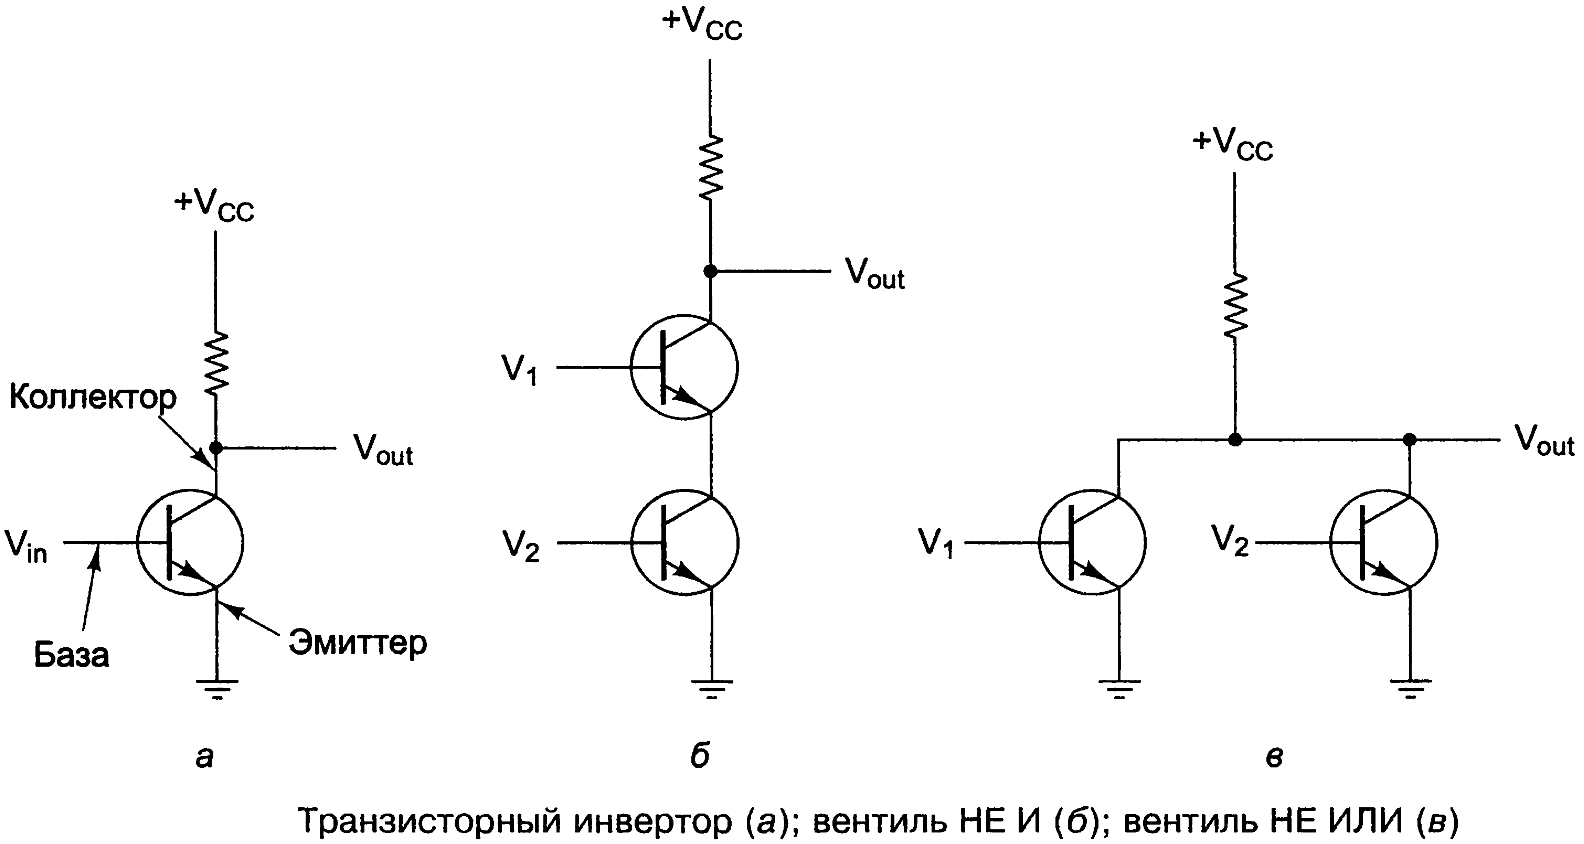
\includegraphics[width=0.8\columnwidth]{images/transistors.png}
\end{center}

\emph{Цифровая схема}~--- это схема, в которой есть только два логических значения:~\code{0} или \code{ложь} (сигнал от~0 до 1\,В) и~\code{1} или \code{истина} (сигнал от~2 до 5\,В).

\emph{Вентили}~--- это электронные устройства, которые позволяют получать различные функции от цифровых (двузначных: \code{0} или \code{1}) сигналов. Вентили лежат в основе аппаратного обеспечения, на котором строятся все цифровые компьютеры.

\begin{center}
  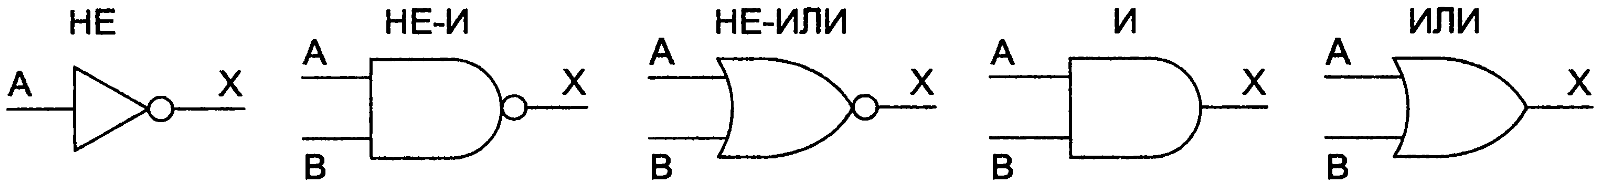
\includegraphics[width=0.8\columnwidth]{images/gates.png}
\end{center}



%%======================
\section{Булевы функции}
%%======================
\emph{Алгебра релейных схем}, \emph{булева функция \(n\) переменных}, \emph{\(2^n\) значений}, \emph{таблица истинности}.

Пример: \(M = f(A,B,C)\)~--- функция большинства, которая принимает 0, если большинство переменных равны 0, и 1, если большинство переменных равны 1.

\begin{center}
\textbf{СДНФ} \(=\) Совершенная Дизъюнктивная Нормальная Форма
\end{center}
\[
  M = \bar ABC + A\bar BC + AB\bar C + ABC
\]

\begin{enumerate}
\item Составить таблицу истинности.
\item Включить инверторы для каждого входного сигнала.
\item Нарисовать вентиль \code{И} для строк таблицы со значением 1.
\item Соединить вентили \code{И} с соответствующими входными сигналами.
\item Вывести выходы всех вентилей \code{И} и направить на вход вентиля \code{ИЛИ}.
\end{enumerate}

\medskip
Любую булеву функцию можно реализовать при помощи вентилей \code{НЕ}, \code{И} и \code{ИЛИ}.



%%================
\WhatToReadSection
%%================
\begin{tabular}{@{}l@{}}
  \citeauthor[глава~1, стр.~2--23, 50--106]{Harris:2015:ru} \\
  \citeauthor[глава~1, стр.~20--26; глава~3, стр.~172--182]{Tanenbaum:2013:ru}
\end{tabular}



%%===============
\ExercisesSection
%%===============
\begin{exercise}
\item Постройте схему для вычисления булевой функции \code{ИСКЛЮЧАЮЩЕЕ-ИЛИ} (\code{XOR}).

\item Реализуйте вентили \code{НЕ}, \code{И} и \code{ИЛИ} на основе \underline{только} вентилей \code{НЕ-ИЛИ}.

\item Реализуйте вентили \code{НЕ}, \code{И} и \code{ИЛИ} на основе \underline{только} вентилей \code{НЕ-И}.

\item Докажите эквивалентность следующих схем
\begin{center}
  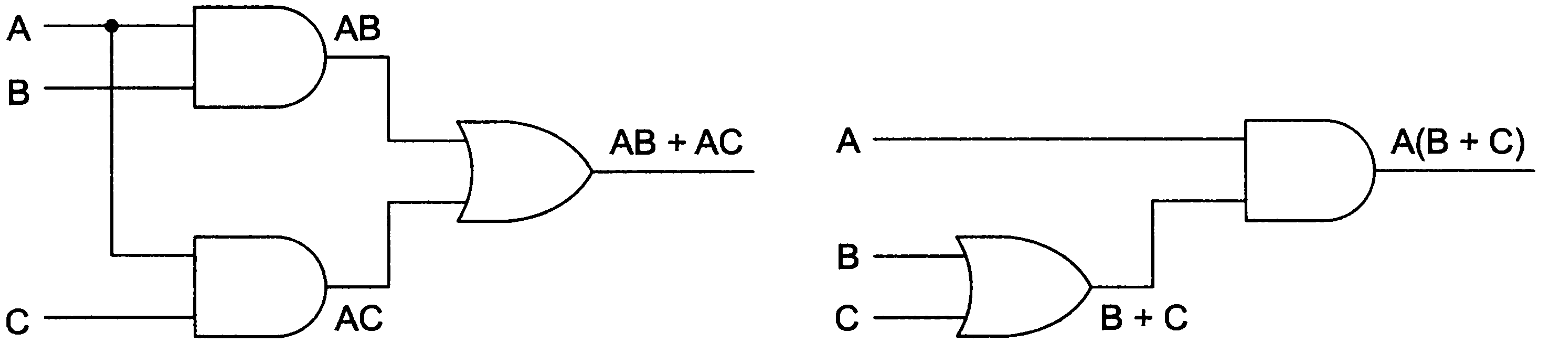
\includegraphics[width=0.8\columnwidth]{images/ex_eq_gates.png}
\end{center}

\end{exercise}

% !TEX encoding   = UTF8
% !TEX spellcheck = ru_RU
% !TEX root = ../seminars.tex

%%==========================================
\chapter{Основные цифровые логические схемы}
%%==========================================

\noindent
\begin{minipage}[c]{0.65\textwidth}
\parindent=2.5em

%%=====================
\section{Мультиплексор}
%%=====================
Схема с \(2^n\) входами, одним выходом и \(n\) линиями управления, которые позволяют выбрать один из входов. Мультиплексоры можно использовать для реализации булевой функции \(n\) переменных.



%%===============
\section{Декодер}
%%===============
Схема, которая получает на входе \(n\)-разрядное число и использует его для того, чтобы выбрать (то есть установить в \code{1}) одну из \(2^n\) выходных линий.

\end{minipage}\hfill\begin{minipage}{0.3\textwidth}

\vspace{-2em}
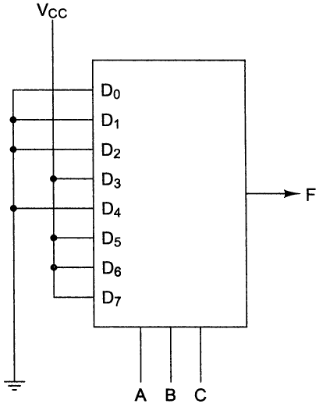
\includegraphics[width=\textwidth]{images/multiplexer.png}

\end{minipage}\medskip



%%==============================================
\section{Арифметико-логическое устройство (АЛУ)}
%%==============================================
\begin{center}
  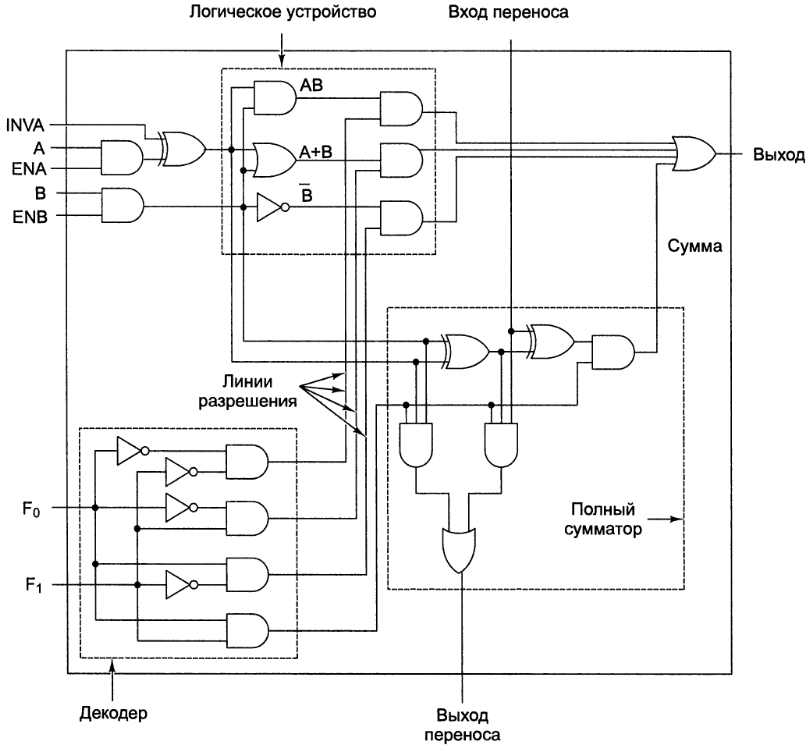
\includegraphics[width=0.8\textwidth]{images/ALU.png}
\end{center}



%%================
\section{Сумматор}
%%================
\emph{Полусумматор}~--- схема для вычисления бита суммы и бита переноса. \emph{Сумматор со сквозным переносом}.



%%==========================
\section{Тактовый генератор}
%%==========================
\noindent\begin{minipage}{0.5\columnwidth}\parindent=2.5em
  Это схема, которая вызывает серию импульсов одинаковой длительности. Интервалы между последовательными импульсами также одинаковы. Временной интервал между началом одного импульса и началом следующего называется \emph{временем такта}.
\end{minipage}\hfill\begin{minipage}{0.46\columnwidth}
  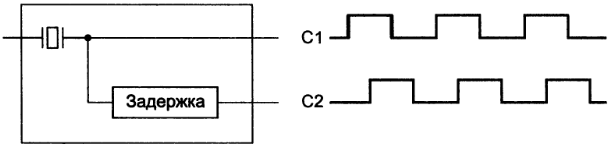
\includegraphics[width=\columnwidth]{images/clock_generator.png}
\end{minipage}

\smallskip
Частота импульсов обычно составляет от 1 до 500\,МГц (время такта от 1000 до 2\,нс). Частота тактового генератора как правило контролируется кварцевым генератором, позволяющим добиться высокой точности. Схемы могут запускаться не только уровнем сигнала, но также фронтом или спадом.



%%=======================
\section{Элементы памяти}
%%=======================
\begin{flushleft}\begin{minipage}[c]{0.3\columnwidth}\newcommand{\vsp}{\vspace{0.5cm}}
    SR-защёлка
    \par\vsp синхронная SR-защёлка
    \par\vsp триггер
    \par\vsp D-триггер
  \end{minipage}\hfill\begin{minipage}[c]{0.65\columnwidth}
    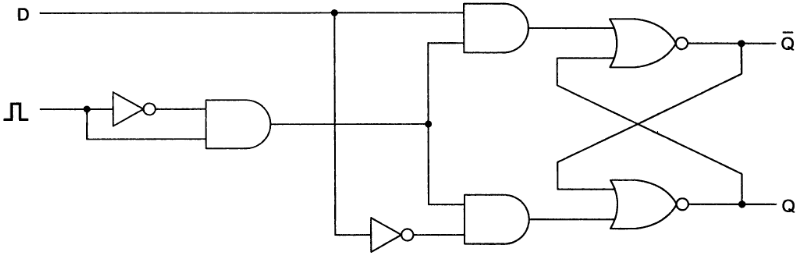
\includegraphics[width=\columnwidth]{images/D-trigger.png}
\end{minipage}\end{flushleft}



%%================
\WhatToReadSection
%%================
\begin{tabular}{@{}l@{}}
  \citeauthor[глава~2, стр.~144--200, 220--248; глава~5, стр.~601--638]{Harris:2015:ru} \\
  \citeauthor[глава~3, стр.~182--208]{Tanenbaum:2013:ru}
\end{tabular}



%%===============
\ExercisesSection
%%===============
\begin{exercise}
\item Постройте двухразрядный \emph{компаратор}, то есть схему, которая получает на вход два двухбитовых слова и выдаёт на выход \code{1}, если слова равны, и \code{0}, если они не равны.

\item \emph{Схема сдвига} имеет \(2^n\) входных битов. Выходные данные~--- это входные данные, сдвинутые на один бит. Линия управления определяет направление сдвига: \code{0}~--- влево, \code{1}~--- вправо. Постройте схему сдвига для четырёхразрядного слова.

\item Нарисуйте логическую схему двухразрядного \emph{кодера}, который содержит 4 входные и 2 выходные линии. Одна из входных линий всегда равна~\code{1}. Двухразрядное двоичное число на двух выходных линиях показывает, какая именно входная линия равна~\code{1}.

\item Нарисуйте логическую схему двухразрядного \emph{демультиплексора}, у которого сигнал на единственной входной линии направляется к одной из четырёх выходных линий в зависимости от значений двух линий управления.

\end{exercise}

% !TEX encoding   = UTF8
% !TEX spellcheck = ru_RU
% !TEX root = ../seminars.tex

%%======================================
\chapter{Простые исполнители алгоритмов}
%%======================================

%%=========================
\section{Конечные автоматы}
%%=========================
Конечные автоматы "--- это простейшие преобразователи входных данных в~выходные данные. Их обычно рассматривают как \emph{потоковые} преобразователи, то есть такие исполнители, которые потенциально могут работать сколь угодно долго, получая на~вход поток символов и печатая на~выход преобразованный поток символов.

\theoremstyle{definition}
\newtheorem{definition}{Определение}

\begin{definition}
  Конечный автомат~\(\mathcal M\) задаётся множеством из~пяти элементов: конечное множество состояний~\(K\), конечный алфавит~\(B\), начальное состояние \(s_0\in K\), подмножество состояний останова \(F\subset K\) и функция перехода \(\pi\colon K\times B \rightarrow K\):
  \[
    \mathcal M = \left\{ B, K, \pi, s_0, F \right\},\quad s_0\in K,~~F\subset K,~~\pi\colon K\times B \rightarrow K.
  \]
\end{definition}

Алгоритм исполнения конечного автомата с~действиями:
\begin{tabbing}
  \(x \leftarrow s_0\) \\
  \codebf{while \(x \notin F\) do} \\
  \quad\= \(b\leftarrow \text{считать символ}\) \\
  \> \(\left(x, a\right)\leftarrow \pi\left(x, b\right)\) \\
  \> выполнить действие \(a\) \\
  \codebf{end while}
\end{tabbing}



%%=======================
\section{Машины Тьюринга}
%%=======================
Можно считать, что машина Тьюринга "--- это обобщённый конечный автомат, в~который добавлены дополнительные элементы:
\begin{itemize}
  \item специальное запоминающее устройство "--- бесконечная лента, состоящая из~ячеек памяти, в~которых могут хранится символы;
  \item возможность совершать определённые действия во~время переходов между состояниями, а именно, двигаться вдоль ленты, читать содержимое ячеек ленты и записывать в~них новые значения.
\end{itemize}

Алгоритм исполнения машин Тьюринга:
\begin{tabbing}
  \(x \leftarrow s_0\) \\
  \codebf{while \(x \notin F\) do} \\
  \quad\= \(b\leftarrow \text{значение активной ячейки}\) \\
  \> \(\left(x, b, a\right)\leftarrow \pi\left(x, b\right)\) \\
  \> \(\text{значение активной ячейки}\leftarrow b\) \\
  \> выполнить действие \(a\) \\
  \codebf{end while}
\end{tabbing}



%%=============================================
\paragraph{Машины Тьюринга и алгорифмы Маркова}
%%=============================================
приведены далее в~нотации консольного эмулятора \name{turingmarkov}\footnote{\url{https://github.com/vslutov/turingmarkov}}, реализованного на~языке \lang{Python}.



%%=================
\paragraph{Пример.}
%%=================
Рассмотрим машину Тьюринга из~упражнения~\ref{ex:turing:parity}, которая реализует счётчик чётности:
\textfile{projects/sem03/parity_counter.turing}

Машина Тьюринга описывается таблицей, где столбцы соответствуют символу на~ленте в~активной ячейке, а каждая строка определяет некоторое состояние:
\begin{flushleft}\begin{tabular}{l@{~~--~~}l}
  0 & движение вправо с~удалением символов, пока количество единиц \textbf{чётно} \\
  1 & то же, пока количество единиц \textbf{нечётно} \\
\end{tabular}\end{flushleft}

Конец слова достигается, когда в~активной ячейке оказывается пробел (обозначаемый символом~<<\_>>). Каждая ячейка определяет значение функции перехода "--- тройку (новый символ, направление движения, новое состояние). Головка может двигаться влево~(L), вправо~(R) или же остаться на~месте~(N). Состояние~<<!>> считается состоянием останова.



%%=========================
\section{Алгорифмы Маркова}
%%=========================
Вычисления, основанные на~правилах, называются продукционными. Исполнитель алгорифмов Маркова "--- это простейший исполнитель, осуществляющий продукционные вычисления.

В~памяти этого исполнителя хранится одно слово~\(X\) конечной длины, составленное из~букв конечного алфавита~\(B\prime\). Оно изначально равно входному слову, а после останова "--- выходному слову (результату вычислений).

Алфавит входного слова~\(B\) является подмножеством алфавита~\(B\prime\). Так же как и в~машинах Тьюринга, во~время вычислений можно использовать дополнительные буквы из~\(B\prime\backslash B\), которые не~могут присутствовать во~входном слове.

Преобразование слова~\(X\) на~исполнителе алгорифмов Маркова происходит путём последовательности преобразований "--- замен одного подслова в~слове~\(X\) на~другое. Возможные замены описываются \textbf{правилами подстановки}.

Упорядоченное множество правил подстановки задаёт логику работы исполнителя. Совокупность правил и алфавитов~\(B\) и~\(B\prime\) называется \textbf{нормальным алгорифмом Маркова}, или просто \textbf{алгорифмом}.

Пусть~\(b\) и~\(b\prime\) "--- некоторые слова в~алфавите~\(B\prime\). Правило <<\(b\rightarrow b\prime\)>> означает, что первое слева вхождение подслова~\(b\) в~слове~\(X\) следует заменить на~слово~\(b\prime\). Это \textbf{правило} считается \textbf{применимым}, если слово~\(X\) содержит подслово~\(b\). Некоторые правила могут быть помечены как \textbf{правила останова}.

Алгоритм работы исполнителя алгорифмов Маркова:
\begin{tabbing}
  \(i \leftarrow 0\) \\
  \(X \leftarrow X_0\) \\
  \codebf{while true do} \\
  \quad
  \=\codebf{if }\(P_i\) применимо к~\(X\)\codebf{ then} \\
  \>\quad
  \=\(X\leftarrow P_i\left(X\right)\) \\
  \>\>\codebf{if }\(P_i\) "--- правило останова\codebf{ then} \\
  \>\>\quad
      \=завершение работы \\
  \>\>\codebf{end if} \\
  \>\>\(i\leftarrow 0\) \\
  \>\codebf{else} \\
  \>\>\(i\leftarrow i + 1\) \\
  \>\>\codebf{if \(i = n\) then} \\
  \>\>\>завершение работы \\
  \>\>\codebf{end if} \\
  \>\codebf{end if} \\
  \codebf{end while}
\end{tabbing}



%%=================
\paragraph{Пример.}
%%=================
Рассмотрим алгорифм из~упражнения~\ref{ex:markov:addx}, который приписывает букву~\(x\) к~входному слову в~алфавите \(B = \left\{0, 1\right\}\) справа:
\textfile[linenos]{projects/sem03/add_x.markov}

Поскольку изначально во~входном слове буква~\(x\) не~может содержаться, то первым сработает последнее правило. Оно заменит пустое подслово (\(b = \emptyset\)), которое содержится в~начале любого слова, на~\(x\). Затем будут срабатывать правила~1 и~2 до~тех пор, пока справа от~\(x\) не~останется ни~одной цифры. Тогда сработает правило~3, которое является правилом останова. Мы не~можем обойтись без~него, так как иначе вновь сработает правило~4 и появится ещё одна буква~\(x\). В~таком случае исполнитель будет работать бесконечно.



%%================
\WhatToReadSection
%%================
\citeauthor[лекции~1--3 и семинары~1--3, стр.~24--60]{Vorozhcov:2008:ru}



%%===============
\ExercisesSection
%%===============
Опишите машины Тьюринга, которые реализуют:
\begin{exercise}[series=statemachine]
\item\label{ex:turing:parity} Счётчик чётности. Выход машины Тьюринга равен~\code{0} или~\code{1} в~зависимости от~того, чётно или нечётно число единиц в~последовательности из~\code{0} и~\code{1}, записанной на~ленте. В~начальном состоянии головка видит первый левый символ.

\item\label{ex:turing:invert} Инверсию заданного слова в~алфавите \code{\{0,1\}}, то есть~\code{0} заменяет на~\code{1}, а~\code{1} "--- на~\code{0}.

\item\label{ex:turing:reverse} <<Переворачивание>> заданного слова в~алфавите \code{\{a,b,c\}}.
\end{exercise}


\bigskip
Запишите нормальные алгорифмы Маркова, которые реализуют:
\begin{exercise}[resume*=statemachine]
\item\label{ex:markov:addx} Приписывание буквы \code{x} к~входному слову в~алфавите \code{\{0,1\}} справа.

\item То же, что и в~упражнении~\ref{ex:turing:invert}.

\item То же, что и в~упражнении~\ref{ex:turing:reverse}.

\item Распознавание правильных скобочных выражений. Правильное скобочное выражение "--- это слово в~алфавите~\code{\{(,)\}}, которое может получиться, если из~арифметического выражения удалить все символы, кроме скобок. Примеры правильных скобочных выражений: пустое слово, \code{()}, \code{(())()}, \code{()()}, \code{((()))}. Примеры неправильных скобочных выражений: \code{)(}, \code{())(()}, \code{(}, \code{))))}, \code{((())}. Результат работы: слово \code{yes}, если скобочное выражение правильное, и слово \code{no} "--- иначе.

\item Увеличение данного натурального числа, записанного в~двоичной системе счисления, на~единицу. Вход: число~\code{n} "--- слово в~алфавите \code{\{0,1\}}. Выход: двоичная запись натурального числа \code{n+1}.
\end{exercise}
% !TEX encoding   = UTF8
% !TEX spellcheck = ru_RU
% !TEX root = ../seminars.tex

%%==================================
\chapter{Представление данных в ЭВМ}
%%==================================

%%===============================
\section{Числа конечной точности}
%%===============================
\vspace{-1\baselineskip}\begin{multicols}{2}\raggedcolumns\columnseprule=0.1pt
  Память компьютера ограничена, поэтому возможно иметь дело только с~такими числами, которые можно представить в~фиксированном количестве разрядов:
  \[
    000,~001,~002,~\ldots,~999
  \]
  Сюда не~входят:
  \begin{itemfeature}
    \item числа большие \(999\)
    \item отрицательные числа
    \item дроби
    \item иррациональные числа
    \item комплексные числа
  \end{itemfeature}
  Свойство замкнутости множества целых чисел:
  \[
    \forall i,j \in \mathbb N :\quad i+j, i-j, i\times j \in \mathbb N
  \]
  Числа конечной точности незамкнуты относительно всех четырёх операций:
  \begin{center}\begin{tabular}{l>{\small}l}
    \(600 + 600 = 1200\) & слишком большое число \\
    \(003 - 005 = -2\)   & отрицательное число \\
    \(050 + 050 = 2500\) & слишком большое число \\
    \(007 / 002 = 3.5\)  & нецелое число \\
  \end{tabular}\end{center}
  Ошибки делятся на~два класса:
  \begin{itemfeature}
    \item ошибки переполнения и ошибки потери значимости
    \item результат не~является членом ряда
  \end{itemfeature}
\end{multicols}

\noindent Законы алгебры для~чисел конечной точности выполняются не~всегда:
\begin{center}\begin{tabular}{lll}
  \(a + (b - c) = (a + b) - c\) & \(700 + (400 - 300) \neq (700 + 400) - 300\) & сочетательный з-н \\
  \(a\times (b - c) = a\times b - a\times c\) & \(5\times (210 - 195) \neq 5\times 210 - 5\times 195\) & распределительный з-н \\
\end{tabular}\end{center}



%%=================================
\section{Отрицательные целые числа}
%%=================================
Системы представления отрицательных \(m\)-разрядных чисел:
\begin{enumerate}
\item со~знаком
\item дополнение до~единицы
\item дополнение до~двух (одно представление нуля: \(+0\), но ряд несимметричен, \(10\ldots0 \to 10\ldots0\))
\item со~смещением на~\(2^{m-1}\)
\end{enumerate}



%%================================
\section{Числа с~плавающей точкой}
%%================================
Экспоненциальная форма: \(n = f\times 10^{e}\). Область значений определяется числом разрядов в~экспоненте~\(e\), а точность~--- числом разрядов в~мантиссе~\(f\).

Для~хранения чисел в~диапазоне \(0.1 \leqslant |f| < 1\) с~трёхразрядной мантиссой со~знаком и двухразрядной экспонентой со~знаком требуется всего~5 разрядов и~2 знака. Характерные промежутки на~числовой оси:
\begin{center}\begin{tabular}{rl}
  \((-\infty, -0.999\times 10^{99})\)               & отрицательное переполнение \\[5pt]
  \([-0.999\times 10^{99}, -0.100\times 10^{-99}]\) & выражаемые отрицательные числа \\[5pt]
  \((-0.100\times 10^{-99}, 0)\)                    & отрицательная потеря значимости \\[5pt]
  \(0\)                                             & нуль \\[5pt]
  \((0, +0.100\times 10^{-99})\)                    & положительная потеря значимости \\[5pt]
  \([+0.100\times 10^{-99}, +0.999\times 10^{99}]\) & выражаемые положительные числа \\[5pt]
  \((+0.999\times 10^{99}, +\infty)\)               & положительное переполнение \\
\end{tabular}\end{center}

Числа не~формируют континуума. Приходится выполнять \emph{округление}. Плотность представляемых чисел разная, но \emph{относительная погрешность} примерно одинаковая.



%%===========================================
\section{Стандарт \texttt{IEEE}~\texttt{754}}
%%===========================================
\noindent\begin{tikzpicture}[bit/.style={inner sep=2pt, font=\footnotesize\ttfamily},
                             num/.style={rectangle, draw, minimum height=6mm, font=\slshape}]
  \node[num, inner xsep=1pt] (signf) {\footnotesize\(\pm\)};
  \node[bit, above=0pt of signf] {1};

  \node[num] (ef) [right=0pt of signf, text width=16mm, align=center] {эксп.};
  \node[bit, above=0.5pt of ef] {8};

  \node[num] (mf) [right=0pt of ef, text width=46mm, align=center] {мантисса};
  \node[bit, above=0.5pt of mf] {23};

  \node[right=3mm of mf] (labf) {одинарная точность};
  \node[bit, above=2pt of labf] {\textbf{32}~бита};


  \node[num, inner xsep=1pt] (signd) [below=6mm of signf] {\footnotesize\(\pm\)};
  \node[bit, above=0pt of signd] {1};

  \node[num] (ed) [right=0pt of signd, text width=22mm, align=center] {эксп.};
  \node[bit, above=0.5pt of ed] {11};

  \node[num] (md) [right=0pt of ed, text width=104mm, align=center] {мантисса};
  \node[bit, above=0.5pt of md] {52};

  \node[right=3mm of md] (labd) {двойная точность};
  \node[bit, above=2pt of labd] {\textbf{64}~бита};
\end{tikzpicture}

\bigskip
Оба формата начинаются со~знакового бита для~всего числа; \texttt{0} указывает на~положительное число, \texttt{1}~--- на~отрицательное. Затем следует смещённая экспонента. Для~формата одинарной точности смещение равно~\(127\), а для~формата двойной точности~--- \(1023\). Минимальная~(\(0\)) и максимальная~(\(255\) и~\(2047\)) экспоненты не~используются для~нормализованных чисел. В~конце идёт мантисса.

\bigskip\hangindent=0.3cm\hangafter=0\noindent
{\newcommand{\numrow}[3]{%
\begin{tabular}{@{}p{5.2cm}|@{}p{3mm}@{}|p{3cm}|p{7.5cm}|}
  \cline{2-4}
  \hfill #1\rule{0pt}{12pt} & \footnotesize $\pm$ & \hfill #2 & \hfill #3 \\
  \cline{2-4}
\end{tabular}}%
\numrow{  нормализованное число}{\(0 < Exp < Max\)}{          любой набор битов}\\[2pt]
\numrow{ненормализованное число}{            \(0\)}{любой ненулевой набор битов}\\[2pt]
\numrow{                   нуль}{            \(0\)}{                      \(0\)}\\[2pt]
\numrow{          бесконечность}{   \(111\ldots1\)}{                        \(0\)}\\[2pt]
\numrow{               не~число}{   \(111\ldots1\)}{любой ненулевой набор битов}
}



%%================
\WhatToReadSection
%%================
\begin{tabular}{@{}l@{}}
  \citeauthor[глава~1 стр.~24--50; глава~5 стр.~639--652]{Harris:2015:ru} \\
  \citeauthor[приложения А и Б стр.~708--728]{Tanenbaum:2013:ru}
\end{tabular}



%%===============
\ExercisesSection
%%===============
\begin{exercise}
\newcommand{\taskcol}[2]{%
  \small%
  \begin{tabular}[t]{@{}l@{}}
  \texttt{#1} \\
  {[Ответ: \texttt{#2}\textsubscript{16}]}
  \end{tabular}%
}
\item Даны десятичные дроби. Представьте их в~формате стандарта \name{IEEE} для~чисел с~плавающей точкой одинарной точности и запишите результат восемью шестнадцатеричными разрядами.

\smallskip
\noindent\begin{enumissue*}[itemjoin=\hfill]
  \item \taskcol  {9.0}{41100000}
  \item \taskcol {5/32}{3E200000}
  \item \taskcol{-5/32}{BE200000}
  \item \taskcol{6.125}{40C40000}
\end{enumissue*}


\renewcommand{\taskcol}[2]{%
  \small%
  \begin{tabular}[t]{@{}l@{}}
  \texttt{#1}\textsubscript{16} \\
  {[Ответ: \texttt{#2}]}
  \end{tabular}%
}
\item Даны числа в~формате стандарта \texttt{IEEE} для~чисел с~плавающей точкой одинарной точности записанные восемью шестнадцатеричными разрядами. Запишите их в~виде десятичных дробей.

\smallskip
\noindent\begin{enumissue*}[itemjoin=\hfill]
  \item \taskcol{42E28000}{113.25}
  \item \taskcol{3F880000}{1.0625}
  \item \taskcol{00800000}{1.17549e-38}
  \item \taskcol{C7F00000}{-122880.0}
\end{enumissue*}


\item Чему равно значение переменной~\code{a} после выполнения следующего оператора?

\cpp/double a = (1. + 1.e-20) - 1.;/

Объясните полученный результат.


\item Дано рекуррентное соотношение:
\[
x_1 = \frac{1}{e},~x_k = 1 - kx_{k-1},\quad k = 2, 3, 4, \ldots
\]
\begin{enumissue}
  \item\hard Докажите, что \(\forall k\in \mathbb N:~x_k > 0\).

  \item Напишите программу, которая вычисляет первые \(15\) чисел с~одинарной точностью и выводит их на~экран.

  \item Объясните противоречие между первыми двумя пунктами.
\end{enumissue}

\end{exercise}

% !TEX encoding   = UTF8
% !TEX spellcheck = ru_RU
% !TEX root = ../seminars.tex

%%==================================================
\chapter{Представление программы на~машинном уровне}
%%==================================================

%%==========================
\section{Процесс компиляции}
%%==========================
\console/$ gcc -Og -o prog p1.c p2.c/%$

\noindent \GCC{} на~самом деле вызывает целый набор программ, чтобы перевести исходный код~\lang{С} в~исполняемый:

\medskip
\begin{itemfeature}
\item\emph{Препроцессор}. Расширяет исходный код, включая содержимое файлов, указанных посредством директивы \code{\#include}, и разворачивая макросы определяемые директивой \code{\#define}.

\item\emph{Компилятор}. Создаёт ассемблерные версии исходных файлов (\code{p1.s}, \code{p2.s}). Ключ (опция)~\hbox{\code{-Og}} предписывает компилятору использовать уровень оптимизации, при~котором получится машинный код, в~целом следующий общей структуре исходного кода на~\lang{C}. Использование более высоких уровней оптимизации (\code{-O1}, \code{-O2} и \code{-O3}) может привести к~генерации машинного кода, который настолько сильно изменён, что понять взаимосвязь с~исходным кодом затруднительно.

\item\emph{Ассемблер}. Переводит ассемблерный код в~объектный (\code{p1.o}, \code{p2.o}). Объектный код является одной из~форм машинного кода "--- он содержит двоичное представление всех команд, но адреса глобальных переменных ещё не определены.

\item\emph{Редактор связей}. Связывает объектные файлы между собой и с~библиотеками функций и создаёт файл \code{prog} (как предписывает ключ \code{-o}\,\code{prog}) с~исполняемым кодом. Исполняемые код "--- ещё одна форма машинного кода, которая может выполняться непосредственно процессором.
\end{itemfeature}



%%====================================
\section{Программа на~машинном уровне}
%%====================================
Компьютерные системы используют ряд абстракций, скрывая детали реализации и предоставляя более простую модель. Наиболее значимые абстракции:

\begin{itemfeature}
  \item \emph{Архитектура набора команд} (ISA "--- \textenglish{Instruction Set Architecture}). Определяет формат и представление программ на~машинном уровне.

  \item \emph{Виртуальные адреса памяти}. Позволяют представить память на~машинном уровне как очень большой массив байтов.
\end{itemfeature}

Ассемблерный код очень близок к~машинному. Основное отличие в~том, что язык ассемблера текстовый и более прост в~понимании для~человека.

Машинный код позволяет увидеть детали и части системы, которые скрыты от~программиста, пишущего на~языке~\lang{C}:

\begin{itemfeature}
  \item \emph{Счётчик команд}, обозначаемый \code{\%rip} в~\name{x86-64}. Определяет последовательность исполнения инструкций.

  \item Целочисленный \emph{файл регистров}. Содержит~16 именованных ячеек памяти для~хранения 64-битных значений. Эти регистры могут хранить адреса (соответствующие указателям в~\lang{C}) или целочисленные данные.

  \item Регистр флагов. Хранит информацию о~результатах последней выполненной арифметической или логической команды. Флаги используются для~реализации условных переходов (\code{if}, \code{while}, \ldots) и пересылки данных по~условию.

  \item Набор векторных регистров. Каждый может хранить одно или несколько целых чисел или чисел с~плавающей точкой.
\end{itemfeature}



\paragraph{Пример.} Рассмотрим следующий код, размещённый в~файле \code{mstore.c}:

\cfile{projects/sem05/mstore.c}

Ассемблерную версию этого кода можно получить, задав компилятору дополнительно ключик~\code{-S}:
\begin{consolecode}
$ gcc -Og -S mstore.c
$ vim mstore.s           # open file with the vim editor
\end{consolecode}

Команды листинга, начинающиеся с~точки, являются директивами ассемблера. Директивы вида \code{.cfi\_*} сохраняют дополнительную информацию, полезную при~отладке программ. Мы можем полностью их игнорировать. Для~отключения генерации этих директив, необходимо добавить ключик \code{-fno-asynchronous-unwind-tables}:

\console/$ gcc -Og -S -fno-asynchronous-unwind-tables mstore.c/%$

Набирать длинную команду каждый раз весьма утомительно. Для~неё можно объявить синоним (\textenglish{alias}):\label{alias:asmlst}

\console/$ alias asmlst="gcc -Og -S -fno-asynchronous-unwind-tables"/%$

\noindent и далее вызывать, используя новое имя:

\console/$ asmlst mstore.c/%$

\noindent В~результате получим ассемблерный листинг из~нашего кода на~\lang{C}:

\gasfile[firstline=5, lastline=11]{projects/sem05/mstore.s}

Ключ~\code{-c} предписывает \GCC{} выполнить и компиляцию, и ассемблирование:

\console/$ gcc -Og -c mstore.c/%$

\noindent Таким образом получается объектный файл (\code{mstore.o}). С помощью отладчика:

\console/$ gdb mstore.o/%$

\noindent можно увидеть машинный код инструкций функции:

\textfile[firstline=16]{projects/sem05/gdb.sh-session}

\noindent Отсюда понятно, что программа, выполняемая машиной,~--- это всего лишь последовательность байтов, кодирующих серию машинных инструкций.

Исследовать содержимое файлов с машинным кодом можно при помощи программ называемых \emph{дизассемблерами}:

\console/$ objdump -d mstore.o/%$

\noindent Из~машинного кода они создают код в~формате похожем на~ассемблерный листинг:

\objdumpfile[firstline=6, lastline=13]{projects/sem05/mstore.c-objdump}

Следует отметить, что:
\begin{itemfeature}
  \item Инструкции \name{x86-64} имеют переменную длину от~1 до~15 байт. Код устроен так, что часто используемые инструкции, а также те, что имеют меньшее количество операндов, занимают меньше байтов.

  \item Формат спроектирован так, что инструкцию можно однозначно декодировать, начиная с~некоторой фиксированной позиции.

  \begin{figure}[h]
    {\centering
      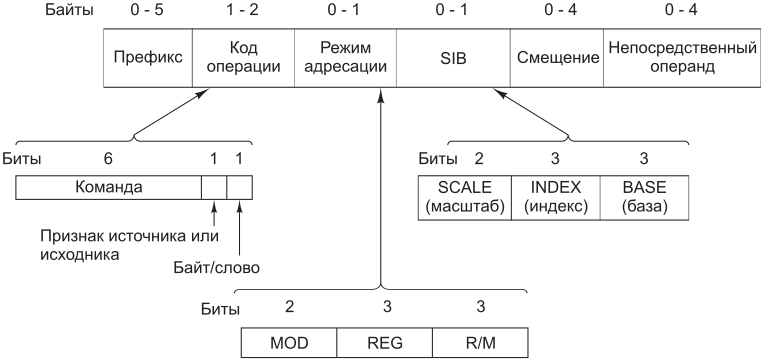
\includegraphics[width=0.8\textwidth]{images/command_format_corei7.png}

    }
    \caption{Формат команд процессора \name{Core}\,\name{i7}}
    \label{fig:cmd:corei7}
  \end{figure}

  \item Дизассемблер выводит ассемблерный код, исходя только из~последовательности байтов в~файле с~машинным кодом.

  \item Дизассемблер использует немного иные соглашения об~именовании, чем \GCC. В~частности, он опускает суффукс~\code{q} у~многих инструкций.
\end{itemfeature}

Чтобы создать код, который будет выполняться системой, необходимо запустить \emph{компоновщик} для~набора объектных файлов, в~одном из~которых определена функция \code{main} (\code{main.cpp}):

\cfile{projects/sem05/main.cpp}

Директива \code{extern "C"} предписывает компилятору использовать соглашения языка~\lang{C} для~именования функций. Язык~\lang{C++} поддерживает <<перегрузку>> имени функции и, вследствие этого, придерживается иных правил об~именовании: он выполняет декорацию (\textenglish{mangling}) исходного имени при~помощи имён типов аргументов.

Собрать исполняемый код можно командой:

\console/$ g++ -Og -o prog main.cpp mstore.o/%$

Объём исполняемого файла значительно больше объёма составляющих его объектных файлов, поскольку он содержит не только код наших процедур, но также информацию, необходимую для~запуска и завершения программы и для~взаимодействия с~операционной системой. Выполнив команду:

\console/$ objdump -d prog/%$

\noindent получим дизассемблерный листинг исполняемого кода:

\objdumpfile[firstline=143, lastline=149]{projects/sem05/prog.c-objdump}

\noindent Какие изменения произошли в~коде функции \code{multstore} при~компоновке?



%%================
\WhatToReadSection
%%================
\citeauthor[глава~3, стр.~190--197]{Bryant:2022:ru}



%%===============
\ExercisesSection
%%===============
\begin{exercise}
\item Настройте рабочую среду, следуя инструкциям из~соответствующего подраздела на~странице~\pageref{sect:workEnv}, если Вы не сделали этого ранее.


\item Рассмотрим следующий код, который пытается просуммировать элементы массива \code{arr}, количество элементов задаётся параметром \code{length}:
\begin{ccode}
/* WARNING: This is buggy code */
float sum_elements (float arr[], unsigned length)
{
  float result = 0.;
  for (int i = 0; i <= length - 1; ++i)
    result += arr[i];

  return result;
}
\end{ccode}

Если вызвать функцию с~аргументом \code{length}, равным \code{0}, то она должна вернуть нуль. Однако вместо этого происходит ошибка при~работе с~памятью. Объясните, почему. Покажите, как исправить код.


\item Рассмотрим следующие \lang{C}-функции:
\begin{ccode}
int fun1 (unsigned word)
{
  return (int) ((word << 24) >> 24);
}

int fun2 (unsigned word)
{
  return ((int) word << 24) >> 24;
}
\end{ccode}

Положим, что они выполняются под~управлением 32-разрядной машины, которая использует арифметику на~основе дополнения до~двух. Также положим, что сдвиг вправо для~чисел со~знаком выполняется арифметически, а для~чисел без~знака "--- логически.
\begin{enumIssue}
  \item Заполните таблицу ниже, которая показывает действие функций на~примере нескольких аргументов. Будет удобнее работать с~числами в~шестнадцатеричной записи. Помните, что цифры от~\code{8} до~\code{F} имеют старший бит равный~\code{1}.

  \begin{flushleft}\ttfamily\small\newcommand*{\ans}{\ansvw}\begin{tabular}{@{}ccc@{}}
    w          & fun1(w)          & fun2(w) \\
    \midrule
    0x00000076 & \ans{0x00000076} & \ans{0x00000076} \\
    0x87654321 & \ans{0x00000021} & \ans{0x00000021} \\
    0x000000C9 & \ans{0x000000C9} & \ans{0xFFFFFFC9} \\
    0xEDCBA987 & \ans{0x00000087} & \ans{0xFFFFFF87} \\
  \end{tabular}\end{flushleft}

  \item Опишите словами, какое полезное вычисление выполняет каждая из~функций.
\end{enumIssue}


\item Вам дали задание написать функцию, которая определяет длиннее ли одна строка, чем другая. Вы решили использовать стандартную функцию \code{strlen}, которая объявляется следующим образом:
\begin{ccode}
/* Prototype for library function strlen */
size_t strlen (const char *s);
\end{ccode}

Вот первая попытка:
\begin{ccode}
/* Determine whether string s is longer than string t */
/* WARNING: This function is buggy */
int strlonger (char *s, char *t)
{
  return strlen(s) - strlen(t) > 0;
}
\end{ccode}

Во время тестирования на~некоторых данных результаты получились неправильные. Вы занялись отладкой и выяснили, что при~компиляции для~32-разрядной архитектуры тип данных \code{size\_t} определён (через \code{typedef}) в~заголовочном файле \code{stdio.h} как \code{unsigned}.
\begin{enumIssue}
  \item В~каких случаях функция выдаёт неверный результат?
  \item Объясните, каким образом этот неверный результат получается.
  \item Покажите, как исправить код, чтобы он работал надёжно.
\end{enumIssue}


\newcommand*{\lstitem}[1]{%
  \makebox[1.5em][r]{\textrm{#1.}}%
}
% O'Hallaron, 3rd ed., problem 2.18
\item Нам будут встречаться листинги, генерируемые дизассемблером "--- программой, которая преобразует исполняемый файл обратно в~более читабельную ASCII форму. Эти файлы содержат много шестнадцатеричных чисел, обычно представленных в~виде дополнения до~двух. Способность распознавать эти числа и понимать их смысл (например, положительные они или отрицательные) представляет собой важный навык.

Преобразуйте шестнадцатеричные значения (в~32-битном дополнении до~двух), представленные в~листинге справа от~мнемоник команд (\code{sub}, \code{mov} и \code{add}) в~десятичные эквиваленты:

{\newcommand*{\ans}{\hfill\ansvw}%
  \objdumpfile[linenos=false, escapeinside=||]{projects/sem05/some_code.c-objdump}
}


% O'Hallaron, 3rd ed., problem 2.44
\item Положим, что \code{int} занимает 32 бита и использует дополнение до~двух для~представления чисел со~знаком. Сдвиги вправо выполняются арифметически для~значений со~знаком и логически для~значений без~знака. Переменные объявлены и инициализированы следующим образом:
\begin{ccode}
int x = foo();  /* Arbitrary value */
int y = bar();  /* Arbitrary value */

unsigned ux = x;
unsigned uy = y;
\end{ccode}

Для~каждого из~следующих~\lang{C} выражений докажите, что оно истинно для~всех значений~\code{x} и~\code{y}, или приведите значения~\code{x} и~\code{y}, для~которых оно ложно:
{\newcommand*{\ans}{\hfill\ansfw{7em}}%
\begin{ccode*}{linenos=false, escapeinside=zz}
  z\lstitem{А}z (x > 0) || (x - 1 < 0) z\ans{min int32\_t}z
  z\lstitem{Б}z (x & 7) != 7 || (x << 29 < 0) z\ans{true}z
  z\lstitem{В}z x * x >= 0 z\ans{0xFFFF}z
  z\lstitem{Г}z x < 0 || -x <= 0 z\ans{true}z
  z\lstitem{Д}z x > 0 || -x >= 0 z\ans{min int32\_t}z
  z\lstitem{Е}z x + y == uy + ux z\ans{true}z
  z\lstitem{Ж}z x * ~y + uy * ux == -x z\ans{true}z
\end{ccode*}
}

\end{exercise}

% !TEX encoding   = UTF8
% !TEX spellcheck = ru_RU
% !TEX root = ../seminars.tex

%%=======================
\chapter{Доступ к~данным}
%%=======================

%%============================================
\section{Структура модуля на~языке ассемблера}
%%============================================
\begin{gascode*}{linenos=false, frame=single}
  .globl   var       # declare var to be visible outside the module
  .bss               # specific [data] section: better-save-space
var:                 # a [label]
  .zero    4         # store 4 bytes, filled by zeroes

  .data              # [data] section
var2:
  .byte    'a'       # store byte, filled with ASCII code of symbol 'a'
var3:
  .long    4         # store 4 bytes, filled with an integer 4

  .text              # [code] section
func:
  mnemonic [op1[, op2[, op3]]]  # an [instruction] format
  # ...
                     # an [empty line] at the end
\end{gascode*}



%%================
\section{Регистры}\label{sect:registers}
%%================
{% registers
\newcommand{\bits}{%
  \tiny\begin{tabular}{p{6cm}p{3cm}p{1.5cm}@{}@{}p{1.5cm}}
    63\hfill & 31 & 15\hfill & ~7\hfill 0 \\
  \end{tabular}}%
%
\newcommand{\cpuReg}[5]{% CPU register
  \begin{tabular}{|p{6cm}|p{3cm}|p{1.5cm}@{}|@{}p{1.5cm}|l}
    \cline{1-4}
    \rule{0pt}{12pt}%
    #1\hfill & #2\hfill & #3 & ~\hfil#4\hfil & \sffamily --\hspace{0.5em}\slshape #5 \\
    \cline{1-4}
  \end{tabular}}%
%
\newcommand{\cpuRegGPe}[2]{% i386 general-purpose CPU register
  \cpuReg{\%r#1x}{\%e#1x}{\%#1x}{\%#1l}{#2}%
}%
\newcommand{\cpuRegSPe}[2]{% i386 specific-purpose CPU register
  \cpuReg{\%r#1}{\%e#1}{\%#1}{\%#1l}{#2}%
}%
\newcommand{\cpuRegGPr}[2]{% x86-64 general-purpose CPU register
  \cpuReg{\%r#1}{\%r#1d}{\%r#1w}{\%r#1b}{#2}%
}%
\newcommand{\cpuRegSPr}[2]{% x86-64 specific-purpose CPU register
  \cpuReg{\%r#1}{\%e#1}{\%#1}{}{#2}%
}%
\ttfamily\small\begin{tabbing}
  \hspace{-0.5cm}\=\bits \\
  \>\cpuRegGPe{a}{accumulator, return value} \\[0.2em]
  \>\cpuRegGPe{b}{base, callee saved} \\[0.2em]
  \>\cpuRegGPe{c}{counter, 4th arg.} \\[0.2em]
  \>\cpuRegGPe{d}{data, 3rd arg.} \\[0.5em]
  %
  \>\cpuRegSPe{si}{source index, 2nd arg.} \\[0.2em]
  \>\cpuRegSPe{di}{destination index, 1st arg.} \\[0.2em]
  \>\cpuRegSPe{bp}{base pointer, callee saved} \\[0.2em]
  \>\cpuRegSPe{sp}{stack pointer} \\[0.5em]
  %
  \>\cpuRegGPr {8}{5th arg.} \\[0.2em]
  \>\cpuRegGPr {9}{6th arg.} \\[0.2em]
  \>\cpuRegGPr{10}{caller saved} \\[0.2em]
  \>\cpuRegGPr{11}{caller saved} \\[0.5em]
  %
  \>\cpuRegGPr{12}{callee saved} \\[0.2em]
  \>\cpuRegGPr{13}{callee saved} \\[0.2em]
  \>\cpuRegGPr{14}{callee saved} \\[0.2em]
  \>\cpuRegGPr{15}{callee saved} \\[1em]
  %
  \>\color{gray}\cpuRegSPr{ip}{instruction pointer} \\[0.2em]
  \>\color{gray}\cpuRegSPr{flags}{condition flags}
\end{tabbing}
}% registers

В~64-разрядном режиме\footcite[3.4.1.1
General-Purpose Registers in~64-Bit Mode]{Intel-v1:2014:en}, размер операнда определяет количество действительных бит в~регистре"~приёмнике:
\begin{itemfeature}
  \item 64-битные операнды порождают 64-битный результат в~регистре"~приёмнике.
  \item 32-битные операнды порождают 32-битный результат, дополняемый нулями до~64-битного значения в регистре"~приёмнике.
  \item 8-~и 16-битные операнды порождают 8-~и 16-битные результаты. Старшие 56~или 48~бит, соответственно, в~регистре"~приёмнике остаются без~изменений. Если 8-~или 16-разрядная операция планируется для~вычисления 64-разрядного адреса, то необходимо в~явном виде дополнить знаковым битом до~полного 64-битного регистра.
\end{itemfeature}



%%=======================
\section{Формы операндов}
%%=======================
\begin{flushleft}
\newcommand*{\E}[1]{r\ensuremath{_{\text{#1}}}}%
\newcommand*{\by}{\ensuremath{\cdot}}%
%
\small\noindent\begin{tabular}{@{}l>{\ttfamily}l>{\ttfamily}ll@{}}
  \toprule
  Тип       & \textrm{Форма}     & \textrm{Значение операнда}     & Адресация \\
  \midrule
  константа & \$Imm              & Imm                            & непосредственная \\[0.5em]

  регистр   & \E{a}              & R[\E{a}]                       & регистровая \\[0.5em]

  память    & Imm                & M[Imm]                         & абсолютная \\
  память    &    (\E{a})         &     M[R[\E{a}]]                & косвенная \\
  память    & Imm(\E{b})         & M[Imm+R[\E{b}]]                & по~базе со~смещением \\
  память    & Imm(\E{b},\E{i})   & M[Imm+R[\E{b}]+R[\E{i}]]       & индексная \\
  память    & Imm(\E{b},\E{i},s) & M[Imm+R[\E{b}]+R[\E{i}]\by{s}] & индексная с~масштабированием \\
  \bottomrule
\end{tabular}\end{flushleft}

Положим, что в~перечисленных ниже адресах памяти и регистрах сохранены указанные значения. Заполните таблицу, вычислив значения операндов.
\begin{center}
  \ttfamily\small
  \begin{tabular}[t]{@{}ll@{}}
    \textrm{Адрес} & \textrm{Значение} \\
    \midrule
    0x100 & 0xFF \\
    0x104 & 0xAB \\
    0x108 & 0x13 \\
    0x10C & 0x11 \\[0.8em]

    \textrm{Регистр} & \textrm{Значение} \\
    \midrule
    \%rax & 0x100 \\
    \%rcx &   0x1 \\
    \%rdx &   0x3 \\
  \end{tabular}\hspace{3cm}
  %
  \newcommand*{\ans}[1]{\ansfw{1.5cm}{#1}}%
  %
  \begin{tabular}[t]{@{}ll@{}}
    \textrm{Операнд} & \textrm{Значение} \\
    \midrule
               \%rax & \ans{0x100} \\
               0x104 & \ans{0xAB} \\
             \$0x108 & \ans{0x108} \\
             (\%rax) & \ans{0xFF} \\
            4(\%rax) & \ans{0xAB} \\
      9(\%rax,\%rdx) & \ans{0x11} \\
    260(\%rcx,\%rdx) & \ans{0x13} \\
      0xFC(,\%rcx,4) & \ans{0xFF} \\
     (\%rax,\%rdx,4) & \ans{0x11} \\
  \end{tabular}
\end{center}



%%==========================
\section{Копирование данных}
%%==========================
{\small\ttfamily\begin{longtable}[l]{@{}lll>{\rmfamily}l@{}}
  \toprule
  \multicolumn{2}{@{}l}{\textrm{Инструкция}} & \textrm{Действие}  & Пояснение \\
  \endfirsthead
  \midrule
  \textbf{mov}   & S,D & D \(\leftarrow\) S & скопировать \\
          movb   &     &                    & \phantom{скопировать} байт \\
          movw   &     &                    & \phantom{скопировать} слово \\
          movl   &     &                    & \phantom{скопировать} двойное слово \\
          movq   &     &                    & \phantom{скопировать} четверное слово \\
  movabsq        & I,R & R \(\leftarrow\) I & \\[0.5em]

  \textbf{movz}  & S,R & R \(\leftarrow\) \textrm{ZeroExtend(\texttt{S})} & скопировать и расширить без~учёта знака \\
          movzbw &     &  & \\
          movzbl &     &  & \\
          movzwl &     &  & \\
          movzbq &     &  & \\
          movzwq &     &  & \\[0.5em]

  \textbf{movs}  & S,R & R \(\leftarrow\) \textrm{SignExtend(\texttt{S})} & скопировать и расширить с~учётом знака \\
          movsbw &     &  & \\
          movsbl &     &  & \\
          movswl &     &  & \\
          movsbq &     &  & \\
          movswq &     &  & \\
          movslq &     &  & \\
  cltq           &     & \%rax \(\leftarrow\) \textrm{SignExtend(\texttt{\%eax})} & \\
  \bottomrule
\end{longtable}}



%%=================
\paragraph{Пример.}
%%=================
Рассмотрим следующий код (\code{move.c}):

\cfile{projects/sem06/move.c}

\noindent Вызвав команду\footnote{Команда-синоним \texttt{asmlst} рассмотрена ранее в~разделе~\ref{alias:asmlst} на~странице~\pageref{alias:asmlst}.}:

\console/$ asmlst move.c/%$

\noindent получим ассемблерный листинг:

\precomment/xp: %rdi, y: %rsi/
\vspace{-1.7\baselineskip}
\gasfile[firstline=5, lastline=8]{projects/sem06/move.s}



%%=====================
\paragraph{Примечания:}
%%=====================
\phantom{some invisible text...}

\smallskip
\begin{enumerate}
\item Пользователи \name{Windows} могут отметить, что у~них в~коде аргументы передаются через регистры \code{\%rcx} и \code{\%rdx}. Это связано с~тем, что разные платформы могут использовать разные соглашения. Чтобы получить листинг в~соглашениях, принятых в~\name{Unix}, добавьте ключ \code{-mabi=sysv}:

\console/$ asmlst -mabi=sysv move.c/%$

\item В~\name{Linux} тип \code{long} означает длинное целое число (8~байт), а под~\name{Windows} это обычное целое число (4~байта). Используйте здесь и далее \code{long}~\code{long} или \code{int64\_t} из~библиотеки \code{<inttypes.h>}.
\end{enumerate}



%%===================================
\section{Работа с~программным стеком}
%%===================================
\begin{flushleft}\small\ttfamily\begin{tabular}[l]{@{}lll>{\rmfamily}l@{}}
  \toprule
  \multicolumn{2}{@{}l}{\textrm{Инструкция}} & \textrm{Действие}  & Пояснение \\
  \midrule
  pushq & S & R[\%rsp]    \(\leftarrow\) R[\%rsp] - 8; & поместить в~стек четверное слово \\
        &   & M[R[\%rsp]] \(\leftarrow\) S             & \\[0.5em]

  popq  & D & D        \(\leftarrow\) M[R[\%rsp]];  & взять из~стека четверное слово \\
        &   & R[\%rsp] \(\leftarrow\) R[\%rsp] + 8  & \\
  \bottomrule
\end{tabular}\end{flushleft}

Чтобы разместить в~стеке четверное слово, необходимо вначале уменьшить указатель стека на~8, а затем записать целевое значение по~новому адресу вершины стека. Таким образом, поведение инструкции \code{pushq~\%rbp} эквивалентно следующей паре инструкций:
\begin{gascode}
  subq $8, %rsp      # decrement stack pointer
  movq %rbp, (%rsp)  # store %rbp on stack
\end{gascode}

\noindent за~исключением того, что инструкция \code{pushq} представляется в~машинном коде всего лишь одним байтом, в~то время как пара инструкций, представленных выше, требует 8~байт.

Чтобы изъять четверное слово из~стека, необходимо вначале прочитать его с~вершины стека, а затем увеличить указатель стека на~8. Таким образом, инструкция \code{popq~\%rax} эквивалентна следующей паре инструкций:
\begin{gascode}
  movq (%rsp), %rax  # read %rax from stack
  addq $8, %rsp      # increment stack pointer
\end{gascode}



%%================
\WhatToReadSection
%%================
\citeauthor[глава~3, стр.~197--209]{Bryant:2022:ru}



%%===============
\ExercisesSection
%%===============
\begin{exercise}
\item Заполните пропущенные суффиксы команды \code{mov}, основываясь на~размере операндов:
{\newcommand*{\ans}{\ansvw}
\begin{gascode*}{texcl}
  mov  %eax, (%rsp)        # \ans{l}
  mov  (%rax), %dx         # \ans{w}
  mov  $0xFF, %bl          # \ans{b}
  mov  (%rsp,%rdx,4), %dl  # \ans{b}
  mov  (%rdx), %rax        # \ans{q}
  mov  %dx, (%rax)         # \ans{w}
\end{gascode*}
}


\item Каждая из~следующих строк вызывает ошибку ассемблера. Поясните, в~чём проблема.
\begin{gascode}
  movb $0xF, (%ebx)
  movl %rax, (%rsp)
  movw (%rax), 4(%rsp)
  movb %al, %sl
  movq %rax, $0x123
  movl %eax, %rdx
  movb %si, 8(%rbp)
\end{gascode}


\item Предположим, что переменные \code{sp} и \code{dp} объявлены как:
\begin{ccode*}{linenos=false}
src_t  *sp;
dest_t *dp;
\end{ccode*}
где \code{src\_t} и \code{dest\_t} некоторые типы данных, объявленные при~помощи \code{typedef}. Мы хотим использовать инструкции копирования, чтобы реализовать операцию:

\cc/*dp = (dest_t) *sp;/

Положим, что значения \code{sp} и \code{dp} размещены в~регистрах \code{\%rdi} и \code{\%rsi}, соответственно. Для каждой записи в~таблице выпишите две инструкции, которые реализуют указанную операцию присваивания. Первая инструкция должна читать данные из~памяти, выполнять требуемое преобразование и записывать соответствующую часть регистра \code{\%rax}. Вторая инструкция затем должна записать эту часть регистра обратно в~память. В~обоих случаях частями могут быть \code{\%rax}, \code{\%eax}, \code{\%ax}, \code{\%al}, и они могут отличаться друг от~друга.

Помните, что при~выполнении преобразования в~\lang{C}, которое включает и изменение размера, и изменение <<знаковости>>, операция должна сначала изменить размер.

\begin{flushleft}\noindent\ttfamily\small
\newcommand*{\w}{12em}%
\newcommand*{\ans}{\ansfw{\w}}%
\begin{tabular}{@{}lll@{}}
  src\_t & dest\_t & \textrm{Инструкция} \\
  \midrule
  long          & long          & \ansfw*{\w}{movq (\%rdi), \%rax} \\
                &               & \ansfw*{\w}{movq	\%rax, (\%rsi)} \\

  char          & int           & \ans{movsbl (\%rdi), \%eax} \\
                &               & \ans{movl   \%eax, (\%rsi)} \\

  char          & unsigned      & \ans{movsbl (\%rdi), \%eax} \\
                &               & \ans{movl   \%eax, (\%rsi)} \\

  unsigned char & long          & \ans{movzbq (\%rdi), \%rax} \\
                &               & \ans{movq   \%rax, (\%rsi)} \\

  int           & char          & \ans{movl (\%rdi), \%eax} \\
                &               & \ans{movb \%al, (\%rsi)} \\

  unsigned      & unsigned char & \ans{movl (\%rdi), \%eax} \\
                &               & \ans{movb \%al, (\%rsi)} \\

  char          & short         & \ans{movsbw (\%rdi), \%ax} \\
                &               & \ans{movw   \%ax, (\%rsi)} \\
\end{tabular}\end{flushleft}


\item Функция имеет прототип:

\cc/void decode (long *xp, long *yp, long *zp);/

и компилируется в~ассемблерный код, приведённый ниже:

\precomment/xp: %rdi, yp: %rsi, zp: %rdx/
\vspace{-0.7\baselineskip}
\gasfile[firstline=5, lastline=12]{projects/sem06/decode.s}

Параметры \code{xp}, \code{yp} и \code{zp} хранятся в~регистрах \code{\%rdi}, \code{\%rsi} и \code{\%rdx}, соответственно. Выпишите эквивалентный исходный~\lang{C} код для~функции \code{decode}.

\end{exercise}

% !TEX encoding   = UTF8
% !TEX spellcheck = ru_RU
% !TEX root = ../seminars.tex

%%============================================
\chapter{Арифметические и логические операции}
%%============================================
Большинство арифметических и логических операций образуют семейства инструкций в~зависимости от~размеров операндов (байт, слово, двойное слово, четверное слово). Исключение составляет инструкция \code{leaq}, у~неё единственный вариант. (Почему?)

\begin{flushleft}\label{tab:cmd:arithlogic}\small\ttfamily\begin{tabular}{@{}lll>{\rmfamily}l@{}}
  \toprule
  \multicolumn{2}{@{}l}{\textrm{Инструкция}} & \textrm{Действие} & Пояснение \\
  \midrule
  leaq & S,R & R \(\leftarrow\) \&S & загрузить действительный адрес \\[0.5em]

  \textbf{inc} & D & D \(\leftarrow\) D + 1 & увеличить на~\code{1} \\
  \textbf{dec} & D & D \(\leftarrow\) D - 1 & уменьшить на~\code{1} \\
  \textbf{neg} & D & D \(\leftarrow\) -D    & изменить знак \\
  \textbf{not} & D & D \(\leftarrow\) \textasciitilde{}D & дополнить до~единиц (поразрядное~\code{НЕ}) \\[0.5em]

  \textbf{add}  & S,D & D \(\leftarrow\) D + S  & сложить \\
  \textbf{sub}  & S,D & D \(\leftarrow\) D - S  & вычесть \\
  \textbf{imul} & S,D & D \(\leftarrow\) D * S  & умножить \\
  \textbf{xor}  & S,D & D \(\leftarrow\) D \textasciicircum{} S & поразрядное \texttt{ИСКЛЮЧАЮЩЕЕ}~\texttt{ИЛИ} \\
  \textbf{or}   & S,D & D \(\leftarrow\) D | S  & поразрядное~\code{ИЛИ} \\
  \textbf{and}  & S,D & D \(\leftarrow\) D \& S & поразрядное~\code{И} \\[0.5em]

  \textbf{sal} & k,D & D \(\leftarrow\) D << k     & сдвиг влево \\
  \textbf{shl} & k,D & D \(\leftarrow\) D << k     & сдвиг влево (то же, что и \code{sal}) \\
  \textbf{sar} & k,D & D \(\leftarrow\) D >>\(_A\) k & арифметический сдвиг вправо \\
  \textbf{shr} & k,D & D \(\leftarrow\) D >>\(_L\) k & логический сдвиг вправо \\
  \bottomrule
\end{tabular}\end{flushleft}



%%=======================================
\section{Загрузка действительного адреса}
%%=======================================
Пусть регистры \code{\%rbx} и \code{\%rdx} хранят значения~\(p\) и~\(q\) соответственно. Заполните таблицу формулами, выражающими значение, которое будет записано в~регистр \code{\%rax}:

\begin{flushleft}\newcommand*{\ans}{\ansfw{2.0cm}}\ttfamily\small\begin{tabular}{@{}ll@{}}
  \textrm{Инструкция} & \textrm{Результат} \\
  \midrule
  leaq 9(\%rdx), \%rax         & \ans{\(9 + q\)} \\
  leaq (\%rdx,\%rbx), \%rax    & \ans{\(q + p\)} \\
  leaq (\%rdx,\%rbx,4), \%rax  & \ans{\(q + 4p\)} \\
  leaq 2(\%rbx,\%rbx,8), \%rax & \ans{\(2 + 9p\)} \\
  leaq 0xE(,\%rdx,2), \%rax    & \ans{\(14 + 2q\)} \\
  leaq 6(\%rbx,\%rdx,8), \%rax & \ans{\(6 + p + 8q\)} \\
\end{tabular}\end{flushleft}



%%===================================
\section{Унарные и бинарные операции}
%%===================================
Положим, что в~перечисленных ниже адресах памяти и регистрах сохранены указанные значения.

Заполните таблицу, указывая регистр или место в~памяти, которые будут изменены в~результате отдельного выполнения каждой инструкции, а также результирующее значение.

\begin{flushleft}
  \small\ttfamily
  \begin{tabular}[t]{@{}ll@{}}
    \textrm{Адрес} & \textrm{Значение} \\
    \midrule
    0x100 & 0xFF \\
    0x108 & 0xAB \\
    0x110 & 0x13 \\
    0x118 & 0x11 \\[0.8em]

    \textrm{Регистр} & \textrm{Значение} \\
    \midrule
    \%rax & 0x100 \\
    \%rcx &   0x1 \\
    \%rdx &   0x3 \\
  \end{tabular}\hfill
  %
  \newcommand*{\ans}{\ansfw{1.3cm}}%
  %
  \begin{tabular}[t]{@{}lll@{}}
    \textrm{Инструкция} & \textrm{Адрес назначения} & \textrm{Значение} \\
    \midrule
    addq \%rcx, (\%rax)         & \ans{0x100} & \ans{0x100} \\
    subq \%rdx, 8(\%rax)        & \ans{0x108} & \ans{0xA8} \\
    imulq \$16, (\%rax,\%rdx,8) & \ans{0x118} & \ans{0x110} \\
    incq 16(\%rax)               & \ans{0x110} & \ans{0x14} \\
    decq \%rcx                  & \ans{\%rcx} & \ans{0x0} \\
    subq \%rdx, \%rax           & \ans{\%rax} & \ans{0xFD} \\
  \end{tabular}
\end{flushleft}



%%======================
\section{Сдвиг разрядов}
%%======================
Ниже приведены~\lang{C} функция:

\cfile{projects/sem07/shift.c}

\noindent и часть её ассемблерного кода, которая выполняет сдвиги и сохраняет результирующее значение в~регистре \code{\%rax}:

{\newcommand*{\ans}{\ansfw{3.45cm}}%
\precomment/x: %rdi, n: %rsi/
\vspace{-1.7\baselineskip}
\begin{gascode*}{escapeinside=||}
  movq %rdi, %rax  # get x
  |\ans{salq \$4, \%rax}|  # x <<= 4
  movl %esi, %ecx  # get n
  |\ans{sarq \%cl, \%rax}|  # x >>= n
\end{gascode*}
}

\noindent Здесь опущены две ключевых инструкции. Выпишите их, опираясь на~комментарии. Сдвиг вправо следует выполнить арифметически.


%%==============
\section{Пример}
%%==============
Рассмотрим код на~\lang{C}, содержащий арифметические вычисления (\code{arith.c}):

\cfile{projects/sem07/arith.c}

\noindent Вызвав \GCC\footnote{Команда-синоним \texttt{asmlst} рассмотрена ранее в~разделе~\ref{alias:asmlst} на~странице~\pageref{alias:asmlst}.}:

\console/$ asmlst arith.c/%$

\noindent получим из~него ассемблерный листинг:

\precomment/x: %rdi, y: %rsi, z: %rdx/
\vspace{-1.7\baselineskip}
\gasfile[firstline=5, lastline=11]{projects/sem07/arith.s}



%%===========================================
\section{Специальные арифметические операции}
%%===========================================
\begin{flushleft}\small\ttfamily\begin{tabular}{@{}lll>{\rmfamily}l@{}}
  \toprule
  \multicolumn{2}{@{}l}{\textrm{Инструкция}} & \textrm{Действие}  & Пояснение \\
  \midrule
  imulq & S & R[\%rdx]R[\%rax] \(\leftarrow\) S \texttimes{} R[\%rax] & полное произведение с~учётом знака \\
  mulq  & S & R[\%rdx]R[\%rax] \(\leftarrow\) S \texttimes{} R[\%rax] & полное произведение без~учёта знака \\[0.5em]

  cqto  &   & R[\%rdx]R[\%rax] \(\leftarrow\) \textrm{SignExtend(\texttt{R[\%rax]})} & расширить до~восьмикратного слова \\[0.5em]

  idivq & S & R[\%rdx] \(\leftarrow\) R[\%rdx]R[\%rax] mod S & деление с~учётом знака \\
        &   & R[\%rax] \(\leftarrow\) R[\%rdx]R[\%rax] \textdiv{} S & \\[0.5em]

  divq  & S & R[\%rdx] \(\leftarrow\) R[\%rdx]R[\%rax] mod S & деление без~учёта знака \\
        &   & R[\%rax] \(\leftarrow\) R[\%rdx]R[\%rax] \textdiv{} S & \\
  \bottomrule
\end{tabular}\end{flushleft}



\paragraph{Примеры.} Рассмотрим следующий код (\code{store\_uprod.c}):

\cfile{projects/sem07/store_uprod.c}

\noindent Используя команду:

\console/$ asmlst store_uproduct.c/%$

\noindent получим ассемблерный листинг. Компилятор использует команду умножения без~учёта знака с~одним аргументом и извлекает результат из~соответствующих регистров:

\precomment/dest: %rdi, x: %rsi, y: %rdx/
\vspace{-1.6\baselineskip}
\gasfile[firstline=5, lastline=10]{projects/sem07/store_uprod.s}


Теперь рассмотрим код, использующий деление (\code{remdiv.c}):

\cfile{projects/sem07/remdiv.c}

\noindent Как и ранее, вызвав команду:

\console/$ asmlst remdiv.c/%$

\noindent получим ассемблерный листинг. Видно, что компилятор использует команду деления, предварительно заполнив соответствующие регистры:

\precomment/x: %rdi, y: %rsi, qp: %rdx, rp: %rcx/
\vspace{-1.7\baselineskip}\label{example:asm:remdiv}
\gasfile[firstline=5, lastline=12]{projects/sem07/remdiv.s}



%%================
\WhatToReadSection
%%================
\citeauthor[глава~3, стр.~209--217]{Bryant:2022:ru}



%%===============
\ExercisesSection
%%===============
\begin{exercise}
\item Дана функция, в~которой опущено вычисляемое выражение:

\begin{ccode}
long scale (long x, long y, long z)
{
  long t = |\ansvw{5*x + 2*y + 8*z}|;
  return t;
}
\end{ccode}

и её ассемблерный код:

\precomment/x: %rdi, y: %rsi, z: %rdx/
\vspace{-0.6\baselineskip}
\gasfile[firstline=5, lastline=9]{projects/sem07/scale.s}

Выпишите пропущенное в~\lang{C} коде выражение.


\item Ниже приведены \lang{C} функция:

{\newcommand*{\ans}[1]{\ansfw{1.6cm}{#1}}
\begin{ccode*}{escapeinside=//}
long arith2 (long x, long y, long z)
{
  long t1 = /\ans{x | y}/;
  long t2 = /\ans{t1 >> 3}/;
  long t3 = /\ans{\textasciitilde{}t2}/;
  long t4 = /\ans{z \textendash{} t3}/;
  return t4;
}
\end{ccode*}
}
и ассемблерный код её тела:\enlargethispage{1\baselineskip}

\precomment/x: %rdi, y: %rsi, z: %rdx/
\vspace{-0.6\baselineskip}
\gasfile[firstline=5, lastline=11]{projects/sem07/arith2.s}

Основываясь на~приведённом коде, восстановите инструкции тела~\lang{C} функции.


\item В~ассемблерном коде, полученном из~\lang{C}, часто можно обнаружить строки вида:

\gas/xorq  %rcx, %rcx/

хотя в~исходном коде никаких операций \code{ИСКЛЮЧАЮЩЕЕ}~\code{ИЛИ} нет.

\begin{enumIssue}
\item Объясните действие данной инструкции. Какую полезную операцию она реализует?

\item Каким образом можно нагляднее выразить эту операцию в~ассемблерном коде?

\item Сравните количество байт, необходимое для~кодирования этих двух реализаций одной и той же операции.
\end{enumIssue}


\item Рассмотрим код функции на~\lang{C}, который вычисляет 128-битное произведение двух 64-битных значений~$x$ и~$y$, а затем сохраняет результат в~память:

\cfile{projects/sem07/store_prod.c}

Ниже показан ассемблерный код, который \GCC{} выдаёт для~этой функции:

\precomment/dest: %rdi, x: %rsi, y: %rdx/
\vspace{-0.6\baselineskip}
\gasfile[firstline=5, lastline=20]{projects/sem07/store_prod.s}

Этот код использует три умножения для~арифметики с~многократно увеличенной точностью, требуемой для~реализации 128-разрядной арифметики на~64-разрядной машине. Опишите алгоритм, который используется для~вычисления произведения, и прокомментируйте ассемблерный код, чтобы показать, как он реализует этот алгоритм.

\smallskip
\emph{Подсказка}: при~расширении аргументов~\(x\) и~\(y\) до~128 бит, их можно представить как:
\[
  x = 2^{64}\cdot x_h + x_l\quad \text{и}\quad y = 2^{64}\cdot y_h + yl,
\]
где \(x_h\), \(x_l\), \(y_h\) и \(y_l\) являются 64-битными значениями. Подобным образом 128-битное произведение может быть записано как:
\[
  p = 2^{64}\cdot p_h + p_l,
\]
где \(p_h\) и \(p_l\) являются 64-битными значениями. Покажите, как вычисляются значения \(p_h\) и \(p_l\) через значения \(x_h\), \(x_l\), \(y_h\) и \(y_l\).


\item Рассмотрим следующую функцию, которая вычисляет частное и остаток от~деления двух 64-битных целых чисел без~знака:

\cfile{projects/sem07/uremdiv.c}

Реализуйте эту функцию, взяв за~основу ассемблерный код для~деления чисел со~знаком, приведённый в~качестве примера на~странице~\pageref{example:asm:remdiv}.

\end{exercise}

% !TEX encoding   = UTF8
% !TEX spellcheck = ru_RU
% !TEX root = ../seminars.tex

%%=====================================
\chapter{Управление потоком выполнения}
%%=====================================

%%=====================
\section{Флаги условий}
%%=====================
В~дополнение к~целочисленным регистрам~ЦП имеет \emph{регистр флагов}, описывающих свойства последней выполненной арифметической или логической операции. Например, предположим, что используется инструкция \code{add} для~выполнения следующей операции:

\cc/int t = a + b;/

\begin{itemfeature}[itemsep=0pt]
  \item[\code{CF}:] \cinline/Carry Flag = (unsigned)t < (unsigned)a/
    \hspace{0.5em} Последняя операция породила перенос из~самого старшего бита. Используется для~обнаружения переполнения при~выполнении операций без~учёта знака.

  \item[\code{ZF}:] \cinline/Zero Flag = (t == 0)/
    \hspace{0.5em} Результатом последней операции стал нуль.

  \item[\code{SF}:] \cinline/Sign Flag = (t < 0)/
    \hspace{0.5em} В~результате последней операции получено отрицательное значение.

  \item[\code{OF}:] \cinline/Overflow Flag = (a < 0 == b < 0) && (t < 0 != a < 0)/
    \hspace{0.5em} Последняя операция над~числами с~учётом знака вызвала переполнение~--- отрицательное или положительное.
\end{itemfeature}

Инструкция \code{leaq} не~изменяет никакие флаги, поскольку подразумевает использование в~адресной арифметике. Остальные операции, приведённые в~таблице на~странице~\pageref{tab:cmd:arithlogic}, производят установку флагов. Логические операции, такие как \code{xor}, устанавливают флаги переноса и переполнения в~нуль. Операции сдвига устанавливают флаг переноса в~значение последнего <<вытесненного>> бита, а флаг переполнения в~нуль. Инструкции \code{inc} и \code{dec} устанавливают флаг переполнения и флаг нуля, но флаг переноса оставляют без~изменений.

В~дополнение к~упомянутым арифметическим и логическим инструкциям есть ещё две инструкции, которые выставляют флаги, не~меняя при~этом никакие другие регистры.

\begin{flushleft}\small\ttfamily\begin{tabular}{@{}lll>{\rmfamily}l@{}}
  \toprule
  \multicolumn{2}{@{}l}{\textrm{Инструкция}} & \textrm{Основана~на}  & Пояснение \\
  \midrule
  \textbf{cmp}  &  S\(_1\),S\(_2\)  &  S\(_2\) \textendash{} S\(_1\) & сравнить \\[0.5em]

  \textbf{test} &  S\(_1\),S\(_2\)  &  S\(_1\) \& S\(_2\)            & протестировать \\
  \bottomrule
\end{tabular}\end{flushleft}

Вместо непосредственного доступа к~значениям флагов существуют три распространённых способа использовать их. В~зависимости от~комбинаций установленных флагов можно:
\begin{enumerate*}[label=\arabic*)]
  \item установить байт в~\code{0} или \code{1},
  \item перейти к~выполнению другой части программы,
  \item скопировать данные.
\end{enumerate*}



%%=====================
\paragraph{Примечания:}
%%=====================
\phantom{some invisible text...}

\smallskip
\begin{enumerate}
  \item Флаг переноса~\code{CF} означает как \emph{перенос} из~старшего разряда, так и \emph{заём}.
  \item Подробнее о~расстановке флагов командами изложено в~руководстве \cite[A.1 EFLAGS AND INSTRUCTIONS]{Intel-v1:2014:en}.
\end{enumerate}



%%==================================
\section{Установка байта по условию}
%%==================================
\begin{flushleft}\small\ttfamily\begin{tabular}{@{}llll>{\rmfamily}l@{}}
  \toprule
  \multicolumn{2}{@{}l}{\textrm{Инструкция}} & \textrm{Синоним} & \textrm{Действие} & Условие \\
  \midrule
  sete   &  D  & setz  & D \(\leftarrow\) ZF & равно/нуль \\
  setne  &  D  & setnz & D \(\leftarrow\) \textasciitilde{}ZF & не~равно/не~нуль \\[0.5em]

  sets   &  D  &       & D \(\leftarrow\) SF & отрицательное \\
  setns  &  D  &       & D \(\leftarrow\) \textasciitilde{}SF & неотрицательное \\[0.5em]

  setg   &  D  & setnle & D \(\leftarrow\) \textasciitilde{}(SF \textasciicircum{} OF) \& \textasciitilde{}ZF & больше (знаковое \(>\)) \\
  setge  &  D  & setnl  & D \(\leftarrow\) \textasciitilde{}(SF \textasciicircum{} OF) & больше или равно (знаковое \(\geqslant\)) \\
  setl   &  D  & setnge & D \(\leftarrow\) SF \textasciicircum{} OF                    & меньше (знаковое \(<\)) \\
  setle  &  D  & setng  & D \(\leftarrow\) (SF \textasciicircum{} OF) | ZF             & меньше или равно (знаковое \(\leqslant\)) \\[0.5em]

  seta   &  D  & setnbe & D \(\leftarrow\) \textasciitilde{}CF \& \textasciitilde{}ZF & выше (беззнаковое \(>\)) \\
  setae  &  D  & setnb  & D \(\leftarrow\) \textasciitilde{}СF                        & выше или равно (беззнаковое \(\geqslant\)) \\
  setb   &  D  & setnae & D \(\leftarrow\) СF                                         & ниже (беззнаковое \(<\)) \\
  setbe  &  D  & setna  & D \(\leftarrow\) CF | ZF                                    & ниже или равно (беззнаковое \(\leqslant\)) \\
  \bottomrule
\end{tabular}\end{flushleft}


%%=================
\paragraph{Пример.}
%%=================
Код функции, имеющей следующий прототип:

\cc/int comp (data_t a, data_t b);/

\noindent вынуждает компилятор генерировать инструкции семейства \code{set}:

\precomment/a: %rdi, b: %rsi/
\vspace{-1.4\baselineskip}
\gasfile[firstline=5, lastline=9]{projects/sem08/comp.s}



%%=====================
\paragraph{Упражнение.}
%%=====================
Код на \lang{C}:

\cfile[linenos=false, firstline=4, lastline=4]{projects/sem08/comp.c}

\noindent выполняет сравнение аргументов~\code{a} и~\code{b}. Тип аргументов задаётся синонимом \code{data\_t} (через \code{typedef}), а операция сравнения~--- макросом \code{COMP} (через \code{\#define}).

Положим, что значение параметра~\code{a} располагается в~соответствующей части регистра \code{\%rdi} и значение параметра~\code{b}~--- регистра \code{\%rsi}. Определите какой тип \code{data\_t} и операция \code{COMP} могли бы заставить компилятор создать код, приведённый ниже. (Правильных ответов может быть несколько, перечислите все.)

\medskip\noindent
\begin{enumissue*}[itemjoin=\hfill]
\item \begin{tabular}[t]{@{}l@{}}
        \gasinline/cmpl  %esi, %edi/ \\
        \gasinline/setl  %al/
      \end{tabular}

\item \begin{tabular}[t]{@{}l@{}}
        \gasinline/cmpw  %si, %di/ \\
        \gasinline/setge %al/
      \end{tabular}

\item \begin{tabular}[t]{@{}l@{}}
        \gasinline/cmpb  %sil, %dil/ \\
        \gasinline/setbe %al/
      \end{tabular}

\item \begin{tabular}[t]{@{}l@{}}
        \gasinline/cmpq  %rsi, %rdi/ \\
        \gasinline/setne %al/
      \end{tabular}
\end{enumissue*}



%%=====================
\paragraph{Упражнение.}
%%=====================
Код на~\lang{C}:

\cfile[linenos=false, firstline=4, lastline=4]{projects/sem08/test.c}

\noindent выполняет сравнение аргумента~\code{a} с~нулём. Тип аргумента задаётся синонимом \code{data\_t} (через \code{typedef}), а операция сравнения~--- макросом \code{TEST} (через \code{\#define}). Значение параметра~\code{a} располагается в~соответствующей части регистра \code{\%rdi}. Определите какой тип \code{data\_t} и операция \code{TEST} могли бы заставить компилятор создать код, приведённый ниже. (Правильных ответов может быть несколько, перечислите все.)

\medskip\noindent
\begin{enumissue*}[itemjoin=\hfill]
\item \begin{tabular}[t]{@{}l@{}}
        \gasinline/testq %rdi, %rdi/ \\
        \gasinline/setge %al/
      \end{tabular}

\item \begin{tabular}[t]{@{}l@{}}
        \gasinline/testw %di, %di/ \\
        \gasinline/sete  %al/
      \end{tabular}

\item \begin{tabular}[t]{@{}l@{}}
        \gasinline/testb %dil, %dil/ \\
        \gasinline/seta  %al/
      \end{tabular}

\item \begin{tabular}[t]{@{}l@{}}
        \gasinline/testl %edi, %edi/ \\
        \gasinline/setle %al/
      \end{tabular}
\end{enumissue*}



%%===========================
\section{Инструкции перехода}
%%===========================
\begin{gascode*}{escapeinside=||}
  movq  $0, %rax     | \comm{set \%rax to 0} |
  jmp .L1            | \comm{goto .L1} |
  movq (%rax), %rax  | \comm{null pointer dereference (skipped)} |
.L1:
  popq %rdx          | \comm{jump target} |
\end{gascode*}

Инструкция \code{jmp .L1} заставляет программу пропустить инструкцию \code{movq} и вместо этого возобновить выполнение, начиная с~инструкции \code{popq}. Во~время генерации объектного кода, ассемблер определяет адреса всех инструкций с~метками и кодирует целевой адрес перехода (значение метки~\code{.L1}) как часть инструкции перехода.

{\small\ttfamily\begin{longtable}[l]{@{}llll>{\rmfamily}l@{}}
  \toprule
  \multicolumn{2}{@{}l}{\textrm{Инструкция}} & \textrm{Синоним} & \textrm{Условие} & Пояснение \\
  \endfirsthead
  \midrule
  jmp & метка    & & 1 & прямой переход \\
  jmp & *операнд & & 1 & косвенный переход \\[0.5em]

  je  & метка & jz   & ZF & равно/нуль \\
  jne & метка & jnz  & \textasciitilde{}ZF & не~равно/не~нуль \\[0.5em]

  js  & метка &      & SF & отрицательное \\
  jns & метка &      & \textasciitilde{}SF & неотрицательное \\[0.5em]

  jg  & метка & jnle & \textasciitilde{}(SF \textasciicircum{} OF) \& \textasciitilde{}ZF & больше (знаковое \(>\)) \\
  jge & метка & jnl  & \textasciitilde{}(SF \textasciicircum{} OF) & больше или равно (знаковое \(\geqslant\)) \\
  jl  & метка & jnge & SF \textasciicircum{} OF                    & меньше (знаковое \(<\)) \\
  jle & метка & jng  & (SF \textasciicircum{} OF) | ZF             & меньше или равно (знаковое \(\leqslant\)) \\[0.5em]

  ja  & метка & jnbe & \textasciitilde{}CF \& \textasciitilde{}ZF & выше (беззнаковое \(>\)) \\
  jae & метка & jnb  & \textasciitilde{}СF                        & выше или равно (беззнаковое \(\geqslant\)) \\
  jb  & метка & jnae & СF                                         & ниже (беззнаковое \(<\)) \\
  jbe & метка & jna  & CF | ZF                                    & ниже или равно (беззнаковое \(\leqslant\)) \\
  \bottomrule
\end{longtable}}

Инструкция \code{jmp} выполняет безусловный переход. Он может быть \emph{прямым}, когда целевой адрес кодируется как часть инструкции (например, \code{jmp .L1}), или \emph{косвенным}, когда целевой адрес перехода читается из~регистра (например, \code{jmp *\%rax}) или из~памяти (например, \code{jmp *(\%rax)}). Остальные инструкции в~таблице представляют собой условный переход. Суффиксы определяются как и для~семейства инструкций \code{set}.



%%==========================================
\subsection{Кодирование инструкций перехода}
%%==========================================
Существует несколько способов представления переходов на~машинном уровне. Один из~наиболее часто используемых~--- запомнить смещение \emph{относительно} адреса следующей команды (\textenglish{program counter relative}). Это смещение может быть представлено, используя~1, 2 или~4 байта. Вторым способом является задание <<абсолютного>> адреса, используя~4 байта для~непосредственного указания целевого адреса.

В~качестве примера относительной адресации рассмотрим следующий код:

\gasfile[firstnumber=1, firstline=6, lastline=13]{projects/sem08/branch.s}

Он содержит два перехода: \code{jmp} в~строке~2 прыгает вперёд к~старшим адресам, в~то время как \code{jg} в~строке~7 прыгает назад к~младшим адресам.

Дизассемблерная версия объектного кода:

\objdumpfile[firstnumber=1, firstline=7, lastline=13]{projects/sem08/branch.c-objdump}

В~аннотациях справа дизассемблер приводит целевой адрес инструкции перехода в~строке~2 как~\code{0x8} и в~строке~5 "--- как~\code{0x5} (дизассемблер выводит все числа в~шестнадцатеричной системе счисления). Однако если взглянуть на~второй байт машинного кода, то в~первом случае видим~\code{0x03}. Добавляя это смещение к~\code{0x5}, адресу следующей инструкции, получим целевой адрес~\code{0x8}, равный адресу инструкции в~строке~4.

Аналогично, целевой адрес второй инструкции перехода представляется в~машинном коде как~\code{0xf8} (десятичное~\code{-8}), используя одно-байтовое дополнение до~двух. Добавляя его к~\code{0xd} (десятичное~\code{13}), адресу инструкции в~строке~6, получим~\code{0x5} "--- адрес инструкции в~строке~3.

Эти примеры показывают, что значение счётчика команд при~выполнении относительной адресации равно адресу следующей инструкции, а не~адресу самой инструкции перехода. Это соглашение восходит к~ранним реализациям, когда процессор обновлял счётчик команд перед выполнением инструкции.

Ниже представлена дизассемблерная версия программы после компоновки:

\objdumpfile[firstnumber=1, firstline=93, lastline=98]{projects/sem08/prog.c-objdump}

Инструкции размещены по~смещённым адресам, но кодировка целевых адресов перехода в~строках~2 и~5 осталась той же. Использование относительной адресации для~переходов позволяет выполнять компактное кодирование инструкций (всего~2 байта) и перемещать объектный код в~памяти без~каких-либо изменений.



%%================
\WhatToReadSection
%%================
\citeauthor[глава~3, стр.~218--225]{Bryant:2022:ru}



%%===============
\ExercisesSection
%%===============
\begin{exercise}
\item Ниже приведены фрагменты из~дизассемблерного листинга исполняемого файла. Некоторые детали заменены~\code{X}-ми. Ответьте на~следующие вопросы:

\begin{enumIssue}
\item Каков целевой адрес инструкции~\code{je}? (Об инструкции \code{callq} ничего знать не~нужно.)
%
\objdumpfile[linenos=false, firstline=1, lastline=2, texcl]{projects/sem08/pc-relative.c-objdump}


\item Каков целевой адрес инструкции~\code{je}?
%
\objdumpfile[linenos=false, firstline=4, lastline=5]{projects/sem08/pc-relative.c-objdump}


\item Каковы адреса инструкций~\code{ja} и \code{pop}?
%
\objdumpfile[linenos=false, firstline=7, lastline=8]{projects/sem08/pc-relative.c-objdump}


\item В~приведённом ниже фрагменте, целевой адрес перехода представлен в~виде~4-х байтового относительного смещения в~формате дополнения до~двух. Байты следуют в~порядке от~младшего к~старшему, отражая обратный порядок байт архитектуры \name{x86-64}. Каков целевой адрес инструкции перехода?
%
\objdumpfile[linenos=false, firstline=10, lastline=11]{projects/sem08/pc-relative.c-objdump}
\end{enumIssue}

\end{exercise}

% !TEX encoding   = UTF8
% !TEX spellcheck = ru_RU
% !TEX root = ../seminars.tex

%%=========================
\chapter{Ветвления и циклы}
%%=========================

%%=====================================
\section{Реализация условных ветвлений}
%%=====================================
Общая форма конструкции \code{if-else} в~\lang{C} задаётся шаблоном:

\begin{ccode*}{linenos=false}
if (|\mystyle{test-expr}|)
  |\mystyle{then-statement}|
else
  |\mystyle{else-statement}|
\end{ccode*}

\noindent где \mystyle{test-expr} является целочисленным выражением, результатом которого является либо нуль (интерпретируется как \code{false}), либо ненулевое значение (интерпретируется как \code{true}). Выполняется только одна из~ветвей: \mystyle{then-statement} или \mystyle{else-statement}.

Эту форму ассемблер обычно реализует в~виде, который можно изобразить, используя синтаксис~\lang{C}, следующим образом:

\begin{ccode*}{linenos=false}
  t = |\mystyle{test-expr}|;
  if (!t)
    goto false;
  |\mystyle{then-statement}|
  goto done;
false:
  |\mystyle{else-statement}|
done:
\end{ccode*}



%%=====================
\paragraph{Упражнение.}
%%=====================
Дана~\lang{C} функция:

\cfile[linenos=false]{projects/sem09/if-else/cond.c}

\noindent для~которой \GCC{} генерирует следующий ассемблерный код:

\precomment/a: %rdi, p: %rsi/
\vspace{-1.6\baselineskip}
\gasfile[firstline=5, lastline=12]{projects/sem09/if-else/cond.s}

\begin{enumIssue}
  \item Напишите \code{goto}-версию на~\lang{C}, которая выполняет те же самые вычисления и отражает поток выполнения ассемблерного кода.

  \item Объясните, почему ассемблерный код содержит два условных ветвления, хотя в~исходном коде~\lang{C} только одна ветвь.
\end{enumIssue}



%%==============================
\section{Копирование по~условию}
%%==============================
Альтернативной стратегией для~реализации условных ветвлений является пересылка данных по~условию. В~этом подходе вычисляются выражения в~обеих ветвях условного оператора, а затем выбирается одно в~зависимости от~выполнения условия. Такая стратегия имеет смысл только в~ограниченных случаях, но она может быть реализована простой инструкцией \emph{копирования по~условию}, которая имеет более высокую производительность на~современных процессорах.

\begin{flushleft}\small\ttfamily\begin{tabular}{@{}llll>{\rmfamily}l@{}}
  \toprule
  \multicolumn{2}{@{}l}{\textrm{Инструкция}} & \textrm{Синоним} & \textrm{Условие} & Пояснение \\
  \midrule
  cmove   & S,R & cmovz  &                  ZF & равно/нуль \\
  cmovne  & S,R & cmovnz & \textasciitilde{}ZF & не~равно/не~нуль \\[0.5em]

  cmovs   & S,R &        &                  SF & отрицательное \\
  cmovns  & S,R &        & \textasciitilde{}SF & неотрицательное \\[0.5em]

  cmovg   & S,R & cmovnle & \textasciitilde{}(SF \textasciicircum{} OF) \& \textasciitilde{}ZF & больше (знаковое $>$) \\
  cmovge  & S,R & cmovnl  & \textasciitilde{}(SF \textasciicircum{} OF) & больше или равно (знаковое $\geqslant$) \\
  cmovl   & S,R & cmovnge & SF \textasciicircum{} OF                    & меньше (знаковое $<$) \\
  cmovle  & S,R & cmovng  & (SF \textasciicircum{} OF) | ZF             & меньше или равно (знаковое $\leqslant$) \\[0.5em]

  cmova   & S,R & cmovnbe & \textasciitilde{}CF \& \textasciitilde{}ZF & выше (беззнаковое $>$) \\
  cmovae  & S,R & cmovnb  & \textasciitilde{}СF                        & выше или равно (беззнаковое $\geqslant$) \\
  cmovb   & S,R & cmovnae & СF                                         & ниже (беззнаковое $<$) \\
  cmovbe  & S,R & cmovna  & CF | ZF                                    & ниже или равно (беззнаковое $\leqslant$) \\
  \bottomrule
\end{tabular}\end{flushleft}

Чтобы понять, как условные операции могут быть реализованы через пересылку данных, рассмотрим следующую общую форму условного выражения с~присваиванием:

\cc/v = |\mystyle{test-expr}| ? |\mystyle{then-expr}| : |\mystyle{else-expr}|;/

Стандартный способ скомпилировать это выражение, используя условные переходы, имеет следующий вид:

\begin{ccode*}{linenos=false}
  if (!|\mystyle{test-expr}|)
    goto false;
  v = |\mystyle{then-expr}|;
  goto done;
false:
  v = |\mystyle{else-expr}|;
done:
\end{ccode*}

Этот код содержит две последовательности команд "--- одну для~вычисления \mystyle{then-expr} и вторую для~вычисления \mystyle{else-expr}. Комбинация условных и безусловных переходов гарантирует, что будет выполнена только одна из~этих последовательностей.

Что касается кода, основанного на~пересылке по~условию, то необходимо вычислять оба выражения: \mystyle{then-expr} и \mystyle{else-expr}. Финальный результат выбирается, в~зависимости от~значения \mystyle{test-expr}:

\begin{ccode*}{linenos=false}
  v  = |\mystyle{then-expr}|;
  ve = |\mystyle{else-expr}|;
  t  = |\mystyle{test-expr}|;
  if (!t) v = ve;
\end{ccode*}

Последняя строка этого кода реализуется операцией пересылки по~условию: зачение~\code{ve} копируется в~\code{v}, только если условие~\code{t} не~выполняется.

Не~все условные выражения могут быть скомпилированы, используя пересылку данных по~условию. Если одно из~выражений условного оператора может вызывать ошибку или имеет побочные эффекты, такой код может привести к~ошибочному поведению:

\cc/long cread (long *xp)  { return xp ? *xp : 0; }/

Использование пересылки по~условию не~всегда повышает производительность кода. Компиляторы должны принимать во~внимание соотношение затрат на~ненужные вычисления и стоимости ошибки в~предсказании перехода (потери на~перезапуск конвейера).



%%=====================
\paragraph{Упражнение.}
%%=====================
Ниже приведена функция на~\lang{C}, в~которой определение операции~\code{OP} не~завершено:

\begin{ccode}
#define OP _____  /* Unknown operator */
long arith (long x)  { return x OP 8; }  |\ansx{\hfill\# Ответ: /}|
\end{ccode}

\noindent При~компиляции \GCC{} генерирует следующий ассемблерный код:

\precomment/x: %rdi/
\vspace{-1.6\baselineskip}
\gasfile[firstline=5, lastline=10]{projects/sem09/if-expr/arith.s}

\begin{enumIssue}
  \item Что использовано в~качестве операции~\code{OP}?
  \item Объясните, как работает этот код.
\end{enumIssue}



%%===============
\ExercisesSection
%%===============
\begin{exercise}

\item Компилируя код на~\lang{C} вида:
{\newcommand*{\ans}{\ansfw{5.5em}}%
\begin{ccode}
long test (long x, long y, long z)
{
  long val = |\ans{z + y - x}|;

  if (|\ans{z > 5}|)
  {
    if (|\ans{y > 2}|)
      val = |\ans{x * z}|;
    else
      val = |\ans{x * y}|;
  }
  else if (|\ans{z < 3}|)
    val = |\ans{y * z}|;

  return val;
}
\end{ccode}
}
\GCC{} генерирует следующий ассемблерный листинг:

\precomment/x: %rdi, y: %rsi, z: %rdx/
\vspace{-0.6\baselineskip}
\gasfile[firstline=5, lastline=25]{projects/sem09/if-else/test.s}

Заполните пропущенные в~\lang{C} коде выражения.



\item Компилируя код на~\lang{C} вида:
{\newcommand*{\ans}{\ansfw{4.5em}}%
\begin{ccode}
long test (long x, long y)
{
  long val = |\ans{12 + y}|;

  if (|\ans{x < 0}|)
  {
    if (|\ans{x < y}|)
      val = |\ans{y - x}|;
    else
      val = |\ans{y \& x}|;
  }
  else if (|\ans{y > 10}|)
    val = |\ans{x + y}|;

  return val;
}
\end{ccode}
}
\GCC{}, запущенный с~ключом \code{-O1}, генерирует следующий ассемблерный листинг:\enlargethispage{1\baselineskip}

\precomment/x: %rdi, y: %rsi/
\vspace{-0.6\baselineskip}
% asmlst -fif-conversion test.c
\gasfile[firstline=5, lastline=20]{projects/sem09/if-expr/test.s}

Заполните пропущенные в~\lang{C} коде выражения.

\end{exercise}



%%=================
% !TEX encoding   = UTF8
% !TEX spellcheck = ru_RU
% !TEX root = ../seminars.tex

%%=============
\section{Циклы}
%%=============
Язык~\lang{C} предоставляет несколько различных циклов: \code{do-while}, \code{while} и \code{for}. В~машинном коде нет соответствующих инструкций. Вместо этого для~реализации таких конструкций используются комбинации условных и безусловных переходов. \GCC{} и другие компиляторы генерируют код для~реализации циклов, придерживаясь двух основных шаблонов, которые будут рассмотрены ниже.



%%=================================
\subsection{Цикл \texttt{do-while}}
%%=================================
Общая форма инструкции \code{do-while} в~\lang{C} задаётся шаблоном:

\begin{ccode*}{linenos=false}
do
  |\mystyle{body-statement}|
  while (|\mystyle{test-expr}|);
\end{ccode*}

\noindent Цикл выполняет тело \mystyle{body-statement}, затем вычисляет условие \mystyle{test-expr} и продолжает работу повторно, пока результатом вычисления условия является не~нуль. Эта форма может быть преобразована в~\code{goto}-версию следующим образом:

\begin{ccode*}{linenos=false}
loop:
  |\mystyle{body-statement}|
  t = |\mystyle{test-expr}|;
  if (t)
    goto loop;
\end{ccode*}



%%=====================
\paragraph{Упражнение.}
%%=====================
Дана~\lang{C} функция:

\cfile{projects/sem09/loop_do_while.c}

\noindent для~которой \GCC{} генерирует следующий ассемблерный код:

\precomment/x initially in %rdi/
\vspace{-1.7\baselineskip}
\gasfile[firstline=5, lastline=15]{projects/sem09/loop_do_while.s}

\begin{enumIssue}
  \item Какие регистры используются для~хранения значений переменных~\code{x}, \code{y} и~\code{n}?
  \item Каким образом компилятор устранил необходимость в~указателе~\code{p} и его разыменовании, которое подразумевает наличие в~коде выражения \code{(*p)+=5}?
  \item Поясните, как ассемблерная версия отображает код на~\lang{C}.
\end{enumIssue}



%%==============================
\subsection{Цикл \texttt{while}}
%%==============================
Общая форма инструкции \code{while} в~\lang{C} задаётся шаблоном:

\begin{ccode*}{linenos=false}
while (|\mystyle{test-expr}|)
  |\mystyle{body-statement}|
\end{ccode*}

\noindent Он отличается от~цикла \code{do-while} тем, что \mystyle{test-expr} вычисляется вначале, и цикл может закончится, не~выполнив \mystyle{body-statement} ни~разу. Существует много способов перевода цикла \code{while} в~машинный код, два из~которых используются в~коде, генерируемом \GCC. Оба способа используют ту же структуру, что и для~\code{do-while}, но отличаются реализацией начальной проверки условия.


%%===============================================
\paragraph{Первый способ <<переход в~середину>>.}
%%===============================================
\enlargethispage{\baselineskip}
\begin{ccode*}{linenos=false}
  goto test;
loop:
  |\mystyle{body-statement}|
test:
  t = |\mystyle{test-expr}|;
  if (t)
    goto loop;
\end{ccode*}


%%=====================
\paragraph{Упражнение.}
%%=====================
Ниже приведена общая структура кода на~\lang{C}:

{\newcommand*{\ans}{\ansfw{10em}}%
%
\begin{ccode*}{linenos=false}
long loop_while (long a, long b)
{
  long result = |\ans{0}|;
  while (|\ans{a > b}|)
  {
    result = |\ans{result + (a + b)}|;
    a = |\ans{a - 1}|;
  }
  return result;
}
\end{ccode*}
}

\noindent для~которой \GCC{} выдаёт следующий код:

\precomment/a: %rdi, b: %rsi/
\vspace{-1.7\baselineskip}
\gasfile[firstline=5, lastline=15]{projects/sem09/loop_while.s}

\noindent Видно, что компилятор использовал переход-в-середину (\textenglish{jump-to-middle}), применив инструкцию \code{jmp} в~строке~7 для~перехода к~проверке условия, которое начинается с~метки~\code{.L2}. Заполните пропущенные части в~\lang{C} коде.



%%=================================================
\paragraph{Второй способ <<защищённый-\code{do}>>.}
%%=================================================
Код преобразуется в~форму \code{do-while} и использует условный переход, чтобы пропустить выполнение тела, если условие сразу не~выполняется:

\begin{ccode*}{linenos=false}
  t = |\mystyle{test-expr}|;
  if (!t)
    goto done;
  do
    |\mystyle{body-statement}|
    while (|\mystyle{test-expr}|);
done:
\end{ccode*}



%%=====================
\paragraph{Упражнение.}
%%=====================
Ниже приведена общая структура кода на~\lang{C}:

{\newcommand*{\ans}{\ansfw{6.5em}}%
%
\begin{ccode*}{linenos=false}
long loop_while2 (long a, long b)
{
  long result = |\ans{b}|;
  while (|\ans{b > 0}|)
  {
    result = |\ans{result * a}|;
    b = |\ans{b - a}|;
  }
  return result;
}
\end{ccode*}
}

\enlargethispage{1.2\baselineskip}
\noindent для~которой \GCC{}, запущенный с~ключом \code{-O1}, выдаёт следующий код:
%
\precomment/a: %rdi, b: %rsi/
\vspace{-1.4\baselineskip}
\gasfile[firstline=5, lastline=17]{projects/sem09/loop_while2.s}

\noindent Видно, что компилятор использовал защищённый-\code{do} (\textenglish{guarded-do}), применив инструкцию \code{jle} в~строке~7 для~пропуска выполнения тела, если условие оказалось невыполненным. Заполните пропущенные части в~\lang{C} коде.



%%================
\WhatToReadSection
%%================
\citeauthor[глава~3, стр.~225--242]{Bryant:2022:ru}



%%===============
\ExercisesSection
%%===============
\begin{exercise}
\item Функция \code{fun\_a} имеет следующую структуру:

{\newcommand*{\ans}{\ansdots}%
%
\begin{ccode}
long fun_a (unsigned long x)
{
  long val = 0;

  while (|\ans{x}|)
  {
    |\ans{val \textasciicircum{}= x;}|
    |\ansx{x >>= 1;}|
  }

  return |\ans{val & 0x1}|;
}
\end{ccode}
}

\GCC{} генерирует для~этой функции ассемблерный код, показанный ниже:

\precomment/x: %rdi/
\vspace{-0.7\baselineskip}
\gasfile[firstline=5, lastline=15]{projects/sem09/fun_a.s}

Разберитесь, как работает этот код, и выполните следующее:

\begin{enumIssue}
\item Определите, какой способ трансляции циклов был использован.
\item При~помощи ассемблерного кода восстановите пропущенные части в~\lang{C}.
\item Опишите словами, что вычисляет функция.
\end{enumIssue}

\end{exercise}

%%=================

%% !TEX encoding   = UTF8
% !TEX spellcheck = ru_RU
% !TEX root = ../seminars.tex

%%=======================================
\chapter{Ветвления и циклы (продолжение)}
%%=======================================

%%=========================
\section{Цикл \texttt{for}}\label{sect:for}
%%=========================
Общая форма инструкции \code{for} в~\lang{C} задаётся шаблоном:

\begin{ccode*}{linenos=false}
for (|\mystyle{init-expr}|; |\mystyle{test-expr}|; |\mystyle{update-expr}|)
  |\mystyle{body-statement}|
\end{ccode*}

\noindent Стандарт языка~\lang{C} утверждает (за~одним исключением, освещаемом в~упражнении~\ref{ex:forcontinue}), что поведение такого цикла идентично следующему коду, использующему цикл \code{while}:

\begin{ccode*}{linenos=false}
|\mystyle{init-expr}|;
while (|\mystyle{test-expr}|)
{
  |\mystyle{body-statement}|
  |\mystyle{update-expr}|;
}
\end{ccode*}

Код, генерируемый \GCC{} для~цикла \code{for}, следует одной из~двух стратегий трансляции, рассмотренных для~цикла \code{while}, в~зависимости от~уровня оптимизации:

\begin{flushleft}\begin{minipage}[t]{0.3\textwidth}
\begin{ccode*}{label=\textrm{переход-в-середину}, frame=topline, framesep=3\fboxsep, linenos=false}
  |\mystyle{init-expr}|;
  goto test;
loop:
  |\mystyle{body-statement}|
  |\mystyle{update-expr}|;
test:
  t = |\mystyle{test-expr}|;
  if (t)
    goto loop;
\end{ccode*}
\end{minipage}\qquad\begin{minipage}[t]{0.3\textwidth}
\begin{ccode*}{label=\textrm{защищённый-\code{do}}, frame=topline, framesep=3\fboxsep, linenos=false}
  |\mystyle{init-expr}|;
  t = |\mystyle{test-expr}|;
  if (!t)
    goto done;
loop:
  |\mystyle{body-statement}|
  |\mystyle{update-expr}|;
  t = |\mystyle{test-expr}|;
  if (t)
    goto loop;
done:
\end{ccode*}
\end{minipage}\end{flushleft}



%%=====================
\paragraph{Упражнение.}
%%=====================
Функция \code{fun\_b} имеет следующую структуру:

{\newcommand*{\ans}{\ansdots}%
%
\begin{ccode*}{linenos=false}
long fun_b (unsigned long x)
{
  long val = 0;
  for (|\ans{long i = 64}|; |\ans{i != 0}|; |\ans{--i}|)
  {
    |\ans{val = (val << 1) \textbar (x \& 0x1);}|
    |\ansx{x >>= 1;}|
  }
  return val;
}
\end{ccode*}
}

\noindent \GCC{} генерирует для~этой функции ассемблерный код, показанный ниже:

\precomment/x: %rdi/
\vspace{-1.7\baselineskip}
\gasfile[firstline=5, lastline=17]{projects/sem10/fun_b.s} % asmlst -O1 fun_b.c

\noindent Разберитесь, как работает этот код, и выполните следующее:
\begin{enumIssue}
\item При~помощи ассемблерного кода восстановите пропущенные части в~\lang{C}.
%\item Объясните, почему нет ни начальной проверки условия перед выполнением тела цикла, ни прыжка к части кода, которая это делает.
\item Опишите словами, что вычисляет функция.
\end{enumIssue}



%%============================================
\section{Реализация оператора \texttt{switch}}
%%============================================
Оператор \code{switch} обеспечивает множественное ветвление на~основе целочисленного значения и особенно полезен, когда имеется большое количество вариантов. Он не~только делает код на~языке~\lang{C} более читабельным, но также допускает эффективную реализацию на~основе структуры данных, называемой \emph{таблицей переходов}. Таблица переходов~--- это массив, в~котором $i$-ый элемент хранит адрес сегмента кода, реализующего некоторое действие программы, соответствующего $i$-му варианту в~операторе \code{switch}. Для~определения целевого адреса перехода код выполняет обращение к~таблице переходов, используя индекс~$i$. Преимущество использования таблицы переходов перед длинной последовательностью иструкций \code{if-else} в~том, что время на~выполнение переключения не~зависит от~количества вариантов. \GCC{} выбирает метод трансляции оператора \code{switch}, руководствуясь количеством вариантов (\textenglish{cases}) и разреженностью значений \code{case}-меток. Таблицы переходов используются, когда имеется несколько вариантов (например, четыре и более), и они укладываются в~небольшой диапазон значений.



%%=====================
\paragraph{Упражнение.}
%%=====================
В~функции на~\lang{C}, которая показана ниже, пропущено тело оператора \code{switch}. \code{case}-метки не~образуют непрерывный диапазон, а некоторые варианты имеют несколько меток.

{\newcommand*{\ans}{\ansdots}%
%
\begin{ccode*}{linenos=false}
void switch2 (long x, long *dest)
{
  long val = 0;
  switch (x)
  {
    |\textcolor{cyan}{...}  \comm{Body of switch statement omitted}|
  }
  *dest = val;
}
\end{ccode*}
}

\noindent При~компиляции этой функции \GCC{} генерирует следующий ассемблерный код для~начальной части процедуры:

\precomment/x: %rdi/
\vspace{-1.7\baselineskip}
\begin{gascode}
switch2:
  addq  $1, %rdi
  cmpq  $8, %rdi
  ja    .L2
  jmp   *.L4(,%rdi,8)
\end{gascode}

\noindent а также код для таблицы переходов:

\begin{gascode}
.L4:
  .quad  .L9
  .quad  .L5
  .quad  .L6
  .quad  .L7
  .quad  .L2
  .quad  .L7
  .quad  .L8
  .quad  .L2
  .quad  .L5
\end{gascode}

\noindent Опираясь на~эти данные, ответьте:
\begin{enumIssue}
\item Какие значения меток были в~операторе \code{switch}?
\item Какие варианты имеют несколько меток в~\lang{C} коде?
\end{enumIssue}



%%================
\WhatToReadSection
%%================
\citeauthor[глава~3, стр.~242--250]{Bryant:2022:ru}



%%===============
\ExercisesSection
%%===============
\begin{exercise}
\item\label{ex:forcontinue} Оператор \code{continue} в~\lang{C} заставляет программу перейти в~конец текущей итерации цикла. Изложенное выше правило перевода цикла \code{for} в~цикл \code{while} требует некоторого уточнения, если в~теле цикла встречается этот оператор. Для~примера рассмотрим следующий код:

\begin{ccode}
/* Example of for-loop containing a continue statement */
/* Sum even numbers between 0 and 9 */
long sum = 0;

for (long i = 0; i < 10; ++i)
{
  if (i & 1)
    continue;

  sum += i;
}
\end{ccode}

\begin{enumIssue}
\item Что получится, если наивно применить упомянутое на~странице~\pageref{sect:for} правило перевода цикла \code{for} в~цикл \code{while}? Что будет неверным?
%
\item Как следует заменить оператор \code{continue} на~оператор \code{goto}, чтобы гарантировать, что цикл \code{while} корректно воспроизводит поведение цикла \code{for}?
\end{enumIssue}


\item Для~функции \code{switcher}, написанной на~\lang{C} и имеющей следующую структуру:

{\newcommand*{\ans}{\ansfw{7.5em}}%
%
\begin{ccode}
void switcher (long a, long b, long c, long *dest)
{
  long val;

  switch (a)
  {
  case |\ans{5}|:      /* Case A */
    c = |\ans{b \textasciicircum 15}|;
    /* Fall through */

  case |\ans{0}|:      /* Case B */
    val = |\ans{c + 112}|;
    break;

  case |\ans{2}|:      /* Case C */
  case |\ans{7}|:      /* Case D */
    val = |\ans{(b + c) << 2}|;
    break;

  case |\ans{4}|:      /* Case E */
    val = |\ans{a}|;
    break;

  default:
    val = |\ans{b}|;
  }

  *dest = val;
}
\end{ccode}
}

\GCC{}, запущенный с~ключом \code{-fno-pie}, генерирует ассемблерный код и таблицу переходов, как показано ниже:\label{ex:jumptable}

\precomment/a: %rdi, b: %rsi, c: %rdx, d: %rcx/
\vspace{-0.6\baselineskip}
\gasfile[firstline=5, lastline=36]{projects/sem10/switcher.s}

Заполните пропущенные части в~\lang{C} коде. Существует только один способ разместить варианты в~шаблоне, за~исключением порядка \code{case}-меток~\code{C} и~\code{D}.

\end{exercise}

%% !TEX encoding   = UTF8
% !TEX spellcheck = ru_RU
% !TEX root = ../seminars.tex

%%=================
\chapter{Процедуры}
%%=================
Процедуры являются ключевой абстракцией в~разработке программного обеспечения. Они предоставляют способ оформления кода, который реализует некоторую функциональность с~заданным набором аргументов и, в случае необходимости, возвращаемым значением. Такая функция может быть вызвана из~другой точки программы. Хорошо спроектированное программное обеспечение использует процедуры как механизм абстракции, скрывая детали реализации и, в~то же время, предоставляя краткий и ясный интерфейс, определяющий, какие значения будут вычислены и какое действие процедура окажет на~состояние программы. Процедуры принимают разные формы в~разных языках программирования "--- функции, методы, подпрограммы, обработчики и т.\,п. "--- но все они обладают общим набором особенностей.

Для~организации процедур на~машинном уровне, необходимо учесть разные моменты. Предположим, что процедура~\code{P} вызывает процедуру~\code{Q}, затем~\code{Q} выполняется и возвращается обратно в~\code{P}. Эти действия включают в~себя один или несколько следующих механизмов:

{\parindent=0.5cm%
%
\smallskip
\hangindent=1.5cm\hangafter=1
\emph{Передача управления.} Счётчик команд должен быть установлен в~адрес первой команды процедуры~\code{Q} при~входе и затем переведён в~адрес первой инструкции~\code{P}, следующей за~вызовом~\code{Q}, при~возврате.

\smallskip
\hangindent=1.5cm\hangafter=1
\emph{Передача данных.} \code{P}~должна быть способна передать один или более параметров в~\code{Q}, а~\code{Q} "--- вернуть значение обратно в~\code{P}.

\smallskip
\hangindent=1.5cm\hangafter=1
\emph{Выделение и освобождение памяти.} \code{Q}~может потребоваться выделить память для~локальных переменных до~начала исполнения и, затем, освободить её перед возвратом.

}



%%========================
\section{Программный стек}
%%========================
Во~время выполнения процедуры~\code{Q} процедура~\code{P}, наряду со~всеми остальными процедурами в~цепочке вызовов, временно приостанавливается. Пока выполняется~\code{Q}, только ей необходимо выделять память под~локальные переменные или аргументы для~вызова другой процедуры. Следовательно, программа может управлять памятью, необходимой для~процедур, используя стек.

В~архитектуре \name{x86-64} стек растёт в~направлении младших адресов. Указатель стека \code{\%rsp} указывает на~вершину стека. Данные могут быть размещены в~стеке и изъяты оттуда, используя команды \code{pushq} и \code{popq}. Место под~данные без~начального значения может быть выделено в~стеке просто путём уменьшения значения указателя стека на~необходимую величину. Освобождение памяти выполняется таким же образом, путём увеличения указателя стека.

Когда процедуре необходимо больше памяти, чем могут хранить регистры, она выделяет место в~стеке. Эта область называется \emph{кадром стека} процедуры. Кадр текущей процедуры всегда расположен на~вершине стека. Когда процедура~\code{P} вызывает~\code{Q} она сохраняет в~стек \emph{адрес возврата}, который указывает, откуда следует возобновить выполнение процедуры~\code{P} после возврата из~\code{Q}. Адрес возврата будем считать частью кадра стека~\code{P}, поскольку он хранит состояние, имеющее значение для~\code{P}. Кадр стека для~большинства процедур имеет фиксированный размер, и память выделяется в~самом начале процедуры. Тем не~менее, для~некоторых процедур необходим стек переменного размера. Процедура~\code{P} может передать до~шести целочисленных значений (т.\,е. указателей и целых чисел) в~регистрах, но если~\code{Q} требует больше аргументов, то они должны быть сохранены в~стеке процедурой~\code{P} перед вызовом~\code{Q}.



%%===========================
\section{Передача управления}
%%===========================
Передача управления из~функции~\code{P} в~функцию~\code{Q} осуществляется установкой указателя команд в~адрес первой команды~\code{Q}. Однако, когда настаёт момент возврата из~\code{Q}, процессору необходима информация, откуда следует возобновить исполнение процедуры~\code{P}.

\begin{flushleft}\small\ttfamily\begin{tabular}{@{}ll>{\rmfamily}l@{}}
  \toprule
  \multicolumn{2}{@{}l}{\textrm{Инструкция}} & Пояснение \\
  \midrule
  \textbf{call} &  метка     &  вызов процедуры (прямой) \\
  \textbf{call} &  *операнд  &  вызов процедуры (косвенный) \\
  \textbf{ret}  &            &  возврат из~процедуры \\
  \bottomrule
\end{tabular}\end{flushleft}

В~машинах с~архитектурой \code{x86-64} эта информация записывается при~вызове процедуры~\code{Q} командой \code{call}~\code{Q}. Данная инструкция помещает адрес~\code{A} в~стек и устанавливает счётчик команд на~начало процедуры~\code{Q}. Адрес~\code{A} называют \emph{адресом возврата} "--- это адрес инструкции, следующей непосредственно за~командой \code{call}. В~дополнение к~команде \code{call} есть инструкция \code{ret}, которая извлекает~\code{A} из~стека и устанавливает счётчик команд в~это значение.



%%=======================
\section{Передача данных}
%%=======================
Первые шесть целочисленных аргументов процедуры размещаются в~регистрах согласно их порядку в~списке аргументов. Аргументы, меньшие 64-х бит, помещаются в~соответствующие части указанных 64-битных регистров.

\begin{flushleft}\small\ttfamily\begin{tabular}{@{}l llllll@{}}
  \toprule
  \multirow{2}{2.5cm}{\rmfamily Размер опе\-ранда, бит} & \multicolumn{6}{c@{}}{\rmfamily Номер аргумента} \\
  \cline{2-7}
  & 1 & 2 & 3 & 4 & 5 & 6 \\
  \midrule
  64 & \%rdi & \%rsi & \%rdx & \%rcx & \%r8  & \%r9 \\
  32 & \%edi & \%esi & \%edx & \%ecx & \%r8d & \%r9d \\
  16 & \%di  & \%si  & \%dx  & \%cx  & \%r8w & \%r9w \\
  8  & \%dil & \%sil & \%dl  & \%cl  & \%r8b & \%r9b \\
  \bottomrule
\end{tabular}\end{flushleft}



%%=====================
\paragraph{Упражнение.}
%%=====================
Функция на~\lang{C} \code{procprob} имеет четыре аргумента~\code{u}, \code{a}, \code{v} и \code{b}. Каждый из~них представляет собой либо число со~знаком, либо указатель на~число со~знаком. Аргументы имеют разные размеры. Ниже приведено тело функции:

\cfile[firstline=3, lastline=5]{projects/sem11/procprob.c}

\noindent Функция компилируется в~следующий код для~архитектуры \code{x86-64}:

\gasfile[firstline=5, lastline=10]{projects/sem11/procprob.s}

\noindent Определите порядок и типы параметров функции. Возможны два верных ответа.



%%===============================================
\section{Размещение локальных переменных в~стеке}
%%===============================================
Причинами размещения локальных переменных в~стеке часто оказываются:
\begin{itemfeature}
  \item Недостаточное количество регистров, чтобы поместить все локальные данные.
  \item К~локальной переменной применяется оператор взятия адреса~\code{\&}, так что компилятор вынужден генерировать адрес для~неё.
  \item Некоторые локальные переменные являются массивами или структурами, и, следовательно, компилятор должен обращаться к~их элементам, используя адресную арифметику и косвенный доступ.
\end{itemfeature}



%%===================================================
\section{Размещение локальных переменных в~регистрах}
%%===================================================
Набор программных регистров действует как разделяемый между всеми процедурами ресурс. Хотя, в~каждый момент времени активна лишь одна из~них, необходима гарантия, что когда одна процедура (\textenglish{caller}) вызывает другую (\textenglish{callee}), последняя не~перезапишет значения некоторых регистров, которые первая планировала использовать далее. По~этой причине в~архитектуре \code{x86-64} принят ряд соглашений об~использовании регистров, которые должны выполняться всеми процедурами, включая библиотечные функции.

По~соглашению, регистры~\code{\%rbx}, \code{\%rbp} и \code{\%r12}~-- \code{\%r15} классифицируются как \textenglish{callee-saved}, то есть их значения обязана сохранить вызываемая процедура. То есть, когда~\code{P} вызывает~\code{Q}, \code{Q} обязана сохранить значения этих регистров такими, какие они были до~её вызова. Процедура~\code{Q} может выполнить это либо не~изменяя их вообще, либо предварительно сохранив их в~стеке, а затем восстановив оттуда обратно. Используя это соглашение код функции~\code{P} может сохранить значение в~любом из~\textenglish{callee-saved} регистров, вызвать~\code{Q}, и затем использовать значение этого регистра без~риска его повреждения за~время вызова.

Все остальные регистры, за~исключением указателя стека~\code{\%rsp}, классифицируются как \textenglish{caller-saved}. Это означает, что они могут изменяться любой функцией. Если процедура~\code{P} хранит некоторые данные в~таком регистре и вызывает процедуру~\code{Q}, то, поскольку~\code{Q} может свободно менять этот регистр, то~\code{P} обязана сама позаботиться о~сохранении этого значения перед вызовом.



%%=========================================================
\section{Соглашения о~вызовах в~\name{Intel}~\name{x86-64}}
%%=========================================================
Опускаясь на~всё более и более низкие уровни абстракции, код становится всё менее переносимым. Так, в~64-битных операционных системах \name{Linux} и \name{Windows} приняты разные соглашения о~вызовах процедур и использовании регистров в~архитектуре \name{Intel}~\name{x86-64}.



{\newcommand{\Reg}[1]{\texttt{\small \%#1}}

%%======================================
\paragraph{\texttt{Linux} \texttt{x64}.}
%%======================================
Соглашения в~\name{Linux} подробно изложены выше (в~данном разделе) и кратко приведены в~таблице раздела~\ref{sect:registers} ранее. Для~удобства повторим эту таблицу ещё раз:
{\small\ttfamily\begin{longtable}[l]{@{}lll@{}}
\toprule
  Регистр & Соглашение & Пояснение \\
\endfirsthead
\midrule
  \Reg{rax} & return value & аккумулятор \\
  \Reg{rbx} & callee saved & база \\
  \Reg{rcx} & 4th argument & счётчик \\
  \Reg{rdx} & 3rd argument & данные \\[0.2em]
%
  \Reg{rsi} & 2nd argument & индекс источника \\
  \Reg{rdi} & 1st argument & индекс приёмника \\
  \Reg{rbp} & callee saved & указатель начала кадра стека процедуры \\
  \Reg{rsp} & stack pointer & \\[0.2em]
%
  \Reg{r8}  & 5th argument & регистр общего назначения \\
  \Reg{r9}  & 6th argument & регистр общего назначения \\
  \Reg{r10} & caller saved & регистр общего назначения \\
  \Reg{r11} & caller saved & регистр общего назначения \\[0.2em]
%
  \Reg{r12} & callee saved & регистр общего назначения \\
  \Reg{r13} & callee saved & регистр общего назначения \\
  \Reg{r14} & callee saved & регистр общего назначения \\
  \Reg{r15} & callee saved & регистр общего назначения \\
\bottomrule
\end{longtable}}



%%========================================
\paragraph{\texttt{Windows} \texttt{x64}.}
%%========================================
Аналогичная таблица для~\name{Windows}:
\begin{flushleft}\begin{tabular}{lll}
\toprule
  Регистр & Соглашение & Пояснение \\
\midrule
  \Reg{rax} & return value & аккумулятор \\
  \Reg{rbx} & callee saved & \\
  \Reg{rcx} & 1st argument & \\
  \Reg{rdx} & 2nd argument & \\[0.2em]
%
  \Reg{rsi} & callee saved & регистр общего назначения \\
  \Reg{rdi} & callee saved & регистр общего назначения \\
  \Reg{rbp} & callee saved & указатель начала кадра стека процедуры \\
  \Reg{rsp} & stack pointer & \\[0.2em]
%
  \Reg{r8}  & 3rd argument & \\
  \Reg{r9}  & 4th argument & \\
  \Reg{r10} & caller saved & используется в~syscall/sysret инструкциях \\
  \Reg{r11} & caller saved & используется в~syscall/sysret инструкциях \\[0.2em]
%
  \Reg{r12} & callee saved & регистр общего назначения \\
  \Reg{r13} & callee saved & регистр общего назначения \\
  \Reg{r14} & callee saved & регистр общего назначения \\
  \Reg{r15} & callee saved & регистр общего назначения \\
\bottomrule
\end{tabular}\end{flushleft}

Первые~4 целочисленных аргумента, размер которых не~превосходит 8~байт, передаются через регистры~\Reg{rcx}, \Reg{rdx}, \Reg{r8}, \Reg{r9}. Остальные аргументы сохраняются в~стек перед вызовом в~обратном порядке, как и в~\name{Linux}.
} % \Reg

На~момент входа в~функцию указатель стека обязан быть выровнен по~границе 16~байт. Это означает, что перед выполнением команды вызова \code{call} указатель стека должен быть кратен 8~байтам, но не~16 одновременно. (Она записывает на~вершину стека адрес возврата, а это те самые 8~байт, которые сделают указатель стека кратным~16.)



%%=============================
\section{Рекурсивные процедуры}
%%=============================

%%=====================
\paragraph{Упражнение.}
%%=====================
Ниже приведена общая структура функции на~\lang{C}:

{\newcommand*{\ans}{\ansfw{4em}}%
  %
  \begin{ccode*}{linenos=false}
    long rfun (unsigned long x)
    {
      if (|\ans{x == 0}|) return |\ans{0}|;

      unsigned long nx = |\ans{x >> 2}|;
      long rv = rfun (nx);

      return |\ans{x + rv}|;
    }
  \end{ccode*}
}

\noindent для которой \GCC{} выдаёт следующий код:

\gasfile[firstline=5, lastline=17]{projects/sem11/rfun.s}

\begin{enumIssue}
  \item Какое значение функция \code{rfun} сохраняет в~\textenglish{callee-saved} регистре \code{\%rbx}?
  \item Заполните пропущенные в~\lang{C} коде выражения.
\end{enumIssue}



%%================
\WhatToReadSection
%%================
\citeauthor[глава~3, стр.~250--264]{Bryant:2022:ru}



%%===============
\ExercisesSection
%%===============
Напишите функцию, которая принимает текстовую строку (в~стиле~\lang{C}) и возвращает~\code{1}, если она оканчивается заглавной латинской буквой, которая более не~встречается в~тексте, и~\code{0} в~противном случае.



%%========================================
\paragraph{Реализация на~языке~\lang{Си}.}
%%========================================
Начать следует с~комментария в~шапке файла \code{check.c}, где полезно привести формулировку проверяемого свойства:

\cfile[lastline=2]{projects/sem11/task/check.c}

Алгоритм проверки прост и состоит из~трёх отдельных действий. Его можно записать следующим образом:

\cfile[firstline=29]{projects/sem11/task/check.c}

\noindent Отметим, что далее предполагается использование компилятора \GCC{} из~пакета \name{MinGW-64} для~ОС \name{Windows}. Чтобы оставаться в~соглашениях \name{SYSV}~\name{ABI}, принятых в~ОС \name{Linux} и которых мы до~сих пор придерживались, перед заголовком функции добавлен соответствующий атрибут. При~компиляции в~\name{Linux} эти атрибуты излишни, их можно опустить.

Вспомогательная функция \code{last\_of()} возвращает последний символ строки~\code{s}:

\cfile[firstline=7, lastline=16]{projects/sem11/task/check.c}

\noindent Мы добавили квалификатор \code{static}, указав компилятору, что функция должна быть видна только в~пределах данного модуля (файла) и недоступна извне. Это одно из~средств сокрытия деталей реализации, которые не~входят в~интерфейс и могут измениться в~новой версии.

Следует помнить о~проверке указателей! Разыменование нулевого указателя недопустимо! Обработка ошибок усложняет логику, и хотелось бы избежать этого в~ассемблерной версии. Простым решением может служить вызов функции \code{abort()} из~\code{<stdlib.h>}. Однако это не~позволяет простым образом выяснить, где произошла ошибка, и требует вывода дополнительного сообщения на~экран.

В~языке~\lang{C++} можно использовать механизм исключений. Хотя, повторить подобные действия компилятора в~ассемблерной версии потребует определённых усилий, в~том числе по~изучению особенностей конкретной платформы. Это остаётся за~рамками нашего курса.

Мы решили вставить проверку предусловия через макрос \code{assert()} из~стандартной библиотеки \code{<assert>}, чтобы напомнить о~важном аспекте при~работе с~указателями. Релиз-версия, как правило, игнорирует такие проверки, объявляя макрос \code{NDEBUG}.

Функция \code{isupper()} реализована в~стандартной библиотеке \code{<ctype.h>} и возвращает~\code{1}, если символ в~верхнем регистре. А функция \code{count()} подсчитывает количество вхождений символа~\code{c} в~строку~\code{s} следующим образом:

\cfile[firstline=18, lastline=27]{projects/sem11/task/check.c}



%%=======================
\paragraph{Тестирование.}
%%=======================
Как всегда, чтобы убедиться в~работоспособности нашей реализации, необходимо написать небольшую <<тестовую оснастку>> (\code{main.cpp}). Для~удобства и выразительности кода определим вспомогательный тип \code{PropertyUnitTest}:

\cppfile[firstline=11, lastline=11]{projects/sem11/task/main.cpp}

\noindent Напомним, что тип \code{pair} из~\code{<utility>} способен хранить пару элементов разного типа. Теперь функция \code{main()} может выглядеть так:

\cppfile[firstline=35]{projects/sem11/task/main.cpp}

Вспомогательная функция \code{max\_width()} возвращает размер наиболее длинной строки среди данных тестов:

\cppfile[firstline=24, lastline=33]{projects/sem11/task/main.cpp}

\noindent Она использует \code{max\_element()} из~стандартной библиотеки шаблонов \code{<algorithm>}. В~данном случае нам необходимо указать, каким образом сравнивать элементы.

И, наконец, функция \code{run()} запускает тест, передавая данные нашей функции

\cppfile[firstline=9, lastline=9]{projects/sem11/task/main.cpp}

\noindent и выводит краткий отчёт об~успешности его выполнения:

\cppfile[firstline=13, lastline=22]{projects/sem11/task/main.cpp}

{\newcommand*{\cpprefurl}{https://en.cppreference.com/w/cpp/string/basic_string}
Отметим, что со~времени выхода стандарта \lang{C++11}, контейнер \href{\cpprefurl}{\code{std::string}}\footnote{\nolinkurl{\cpprefurl}} обязан хранить нулевой байт в~качестве завершающего элемента с~индексом \code{s.size()}.
}



%%=================
\paragraph{Сборка.}
%%=================
Собрать и запустить исполняемый файл можно следующими командами:
\begin{consolecode}
$ gcc -c check.c && g++ -o prog -std=c++17 main.cpp check.o
$ ./prog
\end{consolecode}

\noindent При~успешном выполнении всех тестов мы получим примерно такой вывод на~экране:

\textfile{projects/sem11/task/log}



%%=========================================
\paragraph{Реализация на~языке ассемблера.}
%%=========================================
Код, показанный выше, помогает нам легко и быстро реализовать ассемблерную версию. Мы уже проработали и отладили алгоритм, а также подготовили тесты. Язык ассемблера даёт максимальную свободу при~написании кода, но всю ответственность с~этого момента несёт сам программист, ибо ассемблер не~отслеживает некорректную работу с~типами данных и памятью.

В~шапку файла \code{check\_win-sysv.s} также добавим комментарий с~формулировкой проверяемого свойства:

\gasfile[lastline=2]{projects/sem11/task/check_win-sysv.s}

Интерфейсная функция должна быть доступна извне (директива \code{.globl}):

\gasfile[firstline=33]{projects/sem11/task/check_win-sysv.s}

\noindent Следует помнить о~порядке использования регистров. В~функции \code{check\_property()} мы используем соглашения \name{SYSV}~\name{ABI}, в~то время как функция \code{isupper()} из~стандартной библиотеки уже скомпилирована под~\name{Windows}, и, соответственно, необходимо вызывать её, передавая первый параметр в~регистре \code{\%ecx}, как это принято в~ОС \name{Windows}.

Как видно, мы имеем право смешивать соглашения, ассемблер даёт максимальную гибкость. Но, проверять нас никто не~будет, поэтому необходимо обо всех деталях помнить самому программисту, что значительно усложняет разработку кода. В~противном случае, ошибки неизбежны и заканчиваются неожиданным крахом при~выполнении.

Оставшиеся функции пишем по~шаблону версий на~\lang{Си} в~соглашениях \name{Linux}. Первая функция \code{last\_of()}:

\gasfile[firstline=4, lastline=14]{projects/sem11/task/check_win-sysv.s}

\noindent и вторая функция \code{count()}:

\gasfile[firstline=17, lastline=30]{projects/sem11/task/check_win-sysv.s}

Обе функции локальные, об~этом говорит квалификатор \code{static} при~объявлении в~Си. Поэтому не~нужно давать директиву \code{.globl} для~них. И если не~указано иначе, по~умолчанию мы работаем в~сегменте кода (директива \code{.text}).



%%=======================
\paragraph{Тестирование.}
%%=======================
Собрать исполняемый файл можно одной командой:

\console/$ g++ -o prog -std=c++17 main.cpp check_win-sysv.s/%$

Тестовая оснастка уже готова. Нам остаётся лишь добиться работоспособности кода, чтобы все тесты были успешно выполнены.

%% !TEX encoding   = UTF8
% !TEX spellcheck = ru_RU
% !TEX root = ../seminars.tex

%%==================================
\chapter{Массивы и структуры данных}
%%==================================

%%=====================================
\section{Массивы и адресная арифметика}
%%=====================================

\cc`T A[N];`

Обозначим через~\(x_A\) адрес начала массива. Во-первых, объявление выделяет непрерывную область памяти размером \(L\cdot N\) байт, где~\(L\) "--- размер (в~байтах) данных типа~\(T\). Во-вторых, оно вводит в~область видимости идентификатор~\(A\), который может использоваться как указатель на~начало массива. Доступ к~элементам осуществляется по~индексу в~диапазоне от~\(0\) до~\(N-1\). Элемент с~индексом~\(i\) размещается по~адресу \(x_A + L\cdot i\).



%%=====================
\paragraph{Упражнение.}
%%=====================
Рассмотрим следующие объявления:

\begin{ccode}
int P[5];
short Q[2];
int **R[9];
double *S[10];
short *T[2];
\end{ccode}

Заполните таблицу, описывающую размер элементов, суммарный размер и адрес \(i\)-го элемента для~каждого массива.

\begin{flushleft}\newcommand*{\ans}[1]{\ansfw{3cm}{#1}}%
\texttt\small
\begin{tabular}{@{}lllll@{}}
  \textrm{Массив} & \textrm{Размер элемента} & \textrm{Суммарный размер} & \textrm{Адрес начала} & \textrm{Адрес \(i\)-го элемента} \\
\midrule
  P & \ans{4} & \ans{20} & \(x_P\) & \ans{\(x_P + 4i\)} \\
  Q & \ans{2} & \ans{ 4} & \(x_Q\) & \ans{\(x_Q + 2i\)} \\
  R & \ans{8} & \ans{72} & \(x_R\) & \ans{\(x_R + 8i\)} \\
  S & \ans{8} & \ans{80} & \(x_S\) & \ans{\(x_S + 8i\)} \\
  T & \ans{8} & \ans{16} & \(x_T\) & \ans{\(x_T + 8i\)} \\
\end{tabular}\end{flushleft}



%%=====================
\paragraph{Упражнение.}
%%=====================
Положим, что~\(x_P\) "--- адрес массива~\(P\) типа \code{short} и индекс~\(i\) загружены в~регистры \code{\%rdx} и \code{\%rcx}, соответственно. Для~каждого из~следующих выражений выпишите тип, формулу, определяющую значение, и ассемблерную реализацию. Результат должен быть записан в~регистр \code{\%rax} (или его часть \code{\%ax}).

\begin{flushleft}
\newcommand*{\anst}[1]{\ansfw{1.6cm}{#1}}%
\newcommand*{\ansv}[1]{\ansfw{3cm}{#1}}%
\newcommand*{\ansa}[1]{\ansfw{7cm}{#1}}%
\texttt\small
\begin{tabular}{@{}llll@{}}
  \textrm{Выражение} & \textrm{Тип} & \textrm{Значение} & \textrm{Ассемблерный код} \\
\midrule
  P[1]       & \anst{short}  & \ansv{M[\(x_P + 2\)]}       & \ansa{movw 2(\%rdx), \%ax} \\
  P + 3 + i  & \anst{short*} & \ansv{\(x_P + 2i + 6\)}     & \ansa{leaq 6(\%rdx,\%rcx,2), \%rax} \\
  P[i*4 - 5] & \anst{short}  & \ansv{M[\(x_P + 8i - 10\)]} & \ansa{movw -10(\%rdx,\%rcx,8), \%ax} \\
  P[2]       & \anst{short}  & \ansv{M[\(x_P + 4\)]}       & \ansa{movw 4(\%rdx), \%ax} \\
  \&P[i+2]   & \anst{short*} & \ansv{\(x_P + 2i + 4\)}     & \ansa{leaq 4(\%rdx,\%rcx,2), \%rax} \\
\end{tabular}\end{flushleft}



%%=====================
\paragraph{Упражнение.}
%%=====================
Приведённая ниже функция транспонирует элементы массива \(M\times M\), где \(M\)~определяется при~помощи \code{\#define}:

\cfile[firstline=3]{projects/sem12/transpose.c}

\noindent При~оптимизации с~ключом~\code{-O1} \GCC{} генерирует для~внутреннего цикла следующий код:

\gasfile[firstline=20, lastline=28]{projects/sem12/transpose.s}

\noindent Очевидно, что обращение к~элементам по~индексу \GCC{} преобразовал в~код с~указателями.

\begin{enumIssue}
\item Какой регистр содержит указатель на~элемент массива \code{A[i][j]}?
\item Какой регистр содержит указатель на~элемент массива \code{A[j][i]}?
\item Чему равно значение~\(M\)?
\end{enumIssue}



%%=================
\section{Структуры}
%%=================
Объявление \code{struct} в~\lang{C} создаёт тип данных, который группирует объекты возможно различных типов в~один объект. Доступ к~различным компонентам структуры осуществляется по~имени. Реализация структур подобна реализации массивов в~том, что все компоненты структуры размещаются в~непрерывном участке памяти и указатель на~структуру хранит адрес её первого байта. Компилятор сохраняет информацию о~каждом типе-структуре, запоминая смещения в~байтах каждого поля. Он генерирует ссылки на~элементы структуры, используя эти смещения в~качестве смещений для~инструкций обращения в~память.

В~качестве примера рассмотрим следующее объявление:

\cfile[lastline=7]{projects/sem12/record.c}

\begin{flushleft}
\newcommand*{\col}[2]{\multicolumn{1}{#1}{\scriptsize #2}}
\arrayrulewidth=1pt
\texttt\small
\begin{tabular}{r|c|c|c|c|c|l}
  \col{r}{Offset} & \col{p{2cm}}{0} & \col{p{2cm}}{4} & \col{p{2cm}}{8} & \col{p{2cm}}{} & \col{p{4cm}}{16} & \col{l}{24} \\[-0.1em]
\cline{2-6}
  \scriptsize Contents &\rule{0pt}{1em} i & j & a[0] & a[1] & p & \\
\cline{2-6}
\end{tabular}\end{flushleft}

\noindent и реализацию инструкции:

\cfile[firstline=12, lastline=12]{projects/sem12/record.c}

\noindent полагая, что в~начальный момент значение переменной~\code{r} типа \code{Record*} записано в~регистр \code{\%rdi}:

\gasfile[firstline=6, lastline=10]{projects/sem12/record.s}



%%=====================
\paragraph{Упражнение.}
%%=====================
Рассмотрим объявление структуры:

\cfile[lastline=10]{projects/sem12/st_init.c}

Это объявление показывает, что одна структура может быть встроена в~другую так же, как массивы могут быть встроены внутрь структур и массивов [большей размерности].

Следующая ниже процедура (с~некоторыми опущенными выражениями) выполняет некоторые операции над~приведённой выше структурой:

{\newcommand*{\ans}{\ansfw{5em}}%
%
\begin{ccode*}{linenos=false}
void st_init (struct Test *st)
{
  st->s.y  = |\ans{st.s.x}|;
  st->p    = |\ans{\&st->s.y}|;
  st->next = |\ans{st}|;
}
\end{ccode*}
}

\begin{enumIssue}
  \item Чему равны смещения (в~байтах) следующих полей?

  \begin{flushleft}
  \newcommand*{\ans}{\ansfw{3em}}%
  \texttt\small
  \begin{tabular}{r@{:\quad}l}
    p    & \ans{ 0} \\
    s.x  & \ans{ 8} \\
    s.y  & \ans{12} \\
    next & \ans{16} \\
  \end{tabular}
  \end{flushleft}

  \item Сколько байтов всего занимает экземпляр структуры?

  \item Компилятор генерирует следующий ассемблерный код:

  \gasfile[firstline=5, lastline=11]{projects/sem12/st_init.s}

  На~основе этой информации заполните пропущенные выражения в~коде функции \code{st\_init()}.
\end{enumIssue}



%%====================
\section{Выравнивание}
%%====================
Многие компьютерные системы накладывают ограничения на~допустимые значения адресов для~примитивных (базовых) типов данных, требуя, чтобы адрес объекта был кратен некоторому значению~\(K\) (как правило, \(2\), \(4\) или~\(8\)). Такое \emph{ограничение на~выравнивание} упрощает проектирование аппаратного обеспечения, образующего интерфейс между процессором и системой памяти.

Аппаратное обеспечение \name{x86-64} будет работать корректно вне зависимости от~выравнивания данных. Тем не~менее, \name{Intel} рекомендует выравнивать данные, чтобы улучшить производительность системы памяти. Правило выравнивания основывается на~принципе, что любой примитивный объект, занимающий~\(K\) байт, должен иметь адрес, кратный~\(K\). Из~этого правила вытекает следующая таблица выравниваний:

\begin{flushleft}\small\begin{tabular}{l>{\ttfamily}l}
  \(K\) & \textrm{Типы} \\
\midrule
  \(1\) & char \\
  \(2\) & short \\
  \(4\) & int, float \\
  \(8\) & long, double, char* \\
\end{tabular}\end{flushleft}

Выравнивание осуществляется путём проверки, что каждый тип данных устроен таким образом, что все объекты внутри него удовлетворяют своим ограничениям на~выравнивание. Компилятор размещает директивы в~ассемблерном коде, указывая требуемое выравнивание для~глобальных данных. Например, для~таблицы переходов оператора \code{switch} на~странице \pageref{ex:jumptable}:

\gas`.align 8`

При~работе со~структурами компилятор может выделять больше памяти и оставлять между полями промежутки, чтобы гарантировать, что каждый элемент удовлетворяет своим ограничениям на~выравнивание. Рассмотрим пример:

\begin{ccode*}{linenos=false}
struct S1
{
  int i;
  char c;
  int j;
};
\end{ccode*}

\begin{flushleft}
\newcommand*{\col}[2]{\multicolumn{1}{#1}{\scriptsize #2}}
\arrayrulewidth=1pt
\texttt\small
\begin{tabular}{r|c|c|c|c|l}
  \col{r}{Offset} & \col{p{2cm}}{0} & \col{p{0.5cm}}{4} & \col{p{1.5cm}}{5} & \col{p{2cm}}{8} & \col{l}{12} \\[-0.1em]
\cline{2-5}
  \scriptsize Contents &\rule{0pt}{1em} i & c & \color{cyan} gap & j & \\
\cline{2-5}
\end{tabular}\end{flushleft}

Экземпляр структуры также имеет ограничение на~выравнивание начального адреса. Например, компилятор может добавить промежуток в~конце, чтобы удовлетворить ограничение на~выравнивание элементов в~массиве:

\begin{ccode*}{linenos=false}
struct S2
{
  int i;
  int j;
  char c;
} d[4];
\end{ccode*}

\begin{flushleft}
\newcommand*{\col}[2]{\multicolumn{1}{#1}{\scriptsize #2}}
\arrayrulewidth=1pt
\texttt\small
\begin{tabular}{r|c|c|c|c|l}
  \col{r}{Offset} & \col{p{2cm}}{0} & \col{p{2cm}}{4} & \col{p{0.5cm}}{8} & \col{p{1.5cm}}{9} & \col{l}{12} \\[-0.1em]
  \cline{2-5}
  \scriptsize Contents &\rule{0pt}{1em} i & j & c & \color{cyan} gap & \\
  \cline{2-5}
\end{tabular}\end{flushleft}



%%=====================
\paragraph{Упражнение.}
%%=====================
Для~каждого из~объявлений структуры, определите смещение всех полей, суммарный размер и требование к~выравниванию в~архитектуре \name{x86-64}:

\begin{enumIssue}
  \item \cinline`struct P1 { short i; int c; int *j; short *d; };`
  \item \cinline`struct P2 { int i[2]; char c[8]; short s[4]; long *j; };`
  \item \cinline`struct P3 { long w[2]; int *c[2]; };`
  \item \cinline`struct P4 { char w[16]; char *c[2]; };`
  \item \cinline`struct P5 { struct P4 a[2]; struct P1 t; };`
\end{enumIssue}



%%=========================================================
\HardSection{Выход за~границы памяти и переполнение буфера}
%%=========================================================
Напомним, что ни~язык~\lang{C}, ни~\lang{C++} не~выполняют никаких проверок выхода за~границы массива, а локальные переменные размещаются в~стеке наряду с~\emph{записью активации} "--- информацией о~состоянии программы, такой как значение регистров и адрес возврата. Эта комбинация может привести к~серьёзным ошибкам в~программе, если состояние, сохранённое в~стеке, будет повреждено записью в~<<элемент>> вне массива. Иными словами, когда программа попытается восстановить значение регистра или выполнить инструкцию \code{ret} при~повреждении состояния, дальнейшее выполнение может привести к~серьёзным ошибкам.

Очень распространённый источник повреждения состояния программы известен как \emph{переполнение буфера} (\textenglish{buffer overflow}). При~этом, как правило, создаётся локальный символьный массив для~хранения строки, но размер последней превышает выделенную память. Рассмотрим следующий пример:

\cfile{projects/sem12/echo.c}

Этот код показывает реализацию библиотечной функции \code{gets}, чтобы выявить серьёзную проблему, связанную с~ней. Она читает символы из~стандартного потока ввода в~\code{s} и останавливается, только когда встречает переход на~новую строку или происходит ошибка ввода. Затем завершает считанную строку нулевым байтом. Функция \code{echo} показывает пример использования \code{gets}.

Проблема заключается в~том, что не~существует способа определить, достаточно ли памяти выделено, чтобы вместить считываемую строку.

Исследуя сгенерированный ассемблерный код, можно выяснить структуру кадра стека функции \code{echo}:

\gasfile[firstline=42, lastline=52]{projects/sem12/echo.s} % -fno-stack-protector

По~мере увеличения строки ввода, следующая информация окажется поврежденной:

\begin{flushleft}\begin{tabular}{ll}
  Количество введённых символов & Дополнительное повреждённое состояние \\
\midrule
  \(0-7\)   & ничего \\
  \(8-15\)  & состояние вызывающей функции, регистр \code{\%rbx} \\
  \(16-23\) & адрес возврата \\
  \(24+\)   & состояние вызывающей функции \\
\end{tabular}\end{flushleft}

В~общем случае, использование \code{gets} или любой другой функции, которая может переполнить память, считается плохой практикой программирования. К~несчастью, некоторые часто используемые библиотечные функции, включая \code{strcpy}, \code{strcat} и \code{sprintf}, генерируют последовательность символов в~отсутствие информации о~размере целевого буфера. Такие условия порождают уязвимость к~переполнению буфера.

Более опасное использование переполнения буфера "--- дать программе выполнить нежелательную функцию. Это один из~распространённых приёмов взломать безопасность системы по~сети. Обычно программе скармливается строка, которая содержит выполнимый код, называемый \emph{вредоносным кодом} (\textenglish{exploit code}), и несколько дополнительных байтов, перезаписывающих адрес возврата указателем на~этот код. Выполнение инструкции \code{ret} вызывает переход к~выполнению вредоносного кода.



%%=========================================================
\HardSection{Способы защиты от~атак с~переполнением буфера}
%%=========================================================
Атаки с~переполнением буфера стали настолько распространёнными и вызывали так много проблем с~компьютерными системами, что современные компиляторы и операционные системы внедрили механизмы, чтобы усложнить проведение таких атак и ограничить способы, которыми злоумышленник может захватить управление системой через атаки с~переполнением буфера. Ниже представлены механизмы предоставляемые современными версиями \GCC{} под~\name{Linux}.



%%=============================
\paragraph{Рандомизация стека.}
%%=============================
Чтобы внедрить вредоносный код в~систему, взломщику необходимо вставить не~только сам код, но и указатель на~него как часть заражённой строки. Создание такого указателя требует знания адреса в~стеке, где будет расположена строка. Исторически, адреса в~программном стеке были в~высокой степени предсказуемыми.

Идея \emph{рандомизации стека} заключается в~его размещении по~различным адресам от~одного запуска программы к~другому. Таким образом, даже если множество машин запускают идентичный код, все они будут использовать различные адреса в~стеке. Такое поведение достигается за~счёт выделения случайного количества памяти в~стеке в~промежутке от~\(0\) до~\(n\) при~старте программы, например, при~помощи функции \code{alloca}, которая выделяет указанное ей количество памяти в~стеке. Выделенная память программой не~используется, но вызывает смещение всех последующих адресов в~стеке от~запуска к~запуску. Диапазон выделяемой памяти должен быть достаточно велик, чтобы получить существенные изменения адресов, но, в~то же время, и достаточно мал, чтобы не~расходовать память программы впустую.

Следующий код демонстрирует простой способ определения <<типичного>> адреса в~стеке (\code{stack\_address.cpp}):

\cppfile{projects/sem12/stack_address.cpp}

Собрать и запустить (10~раз) программу можно следующим образом:

\begin{consolecode}
$ g++ -o prog -Og stack_address.cpp
$ for (( i = 0; $i < 10; ++i )) do ./prog; done
stack address is 0x7ffcaf551740
stack address is 0x7fff203c31f0
stack address is 0x7ffdf1b0aea0
stack address is 0x7ffd2a5c0270
stack address is 0x7fff0067d450
stack address is 0x7ffcdc471290
stack address is 0x7fff63c3ff20
stack address is 0x7ffd0b84a910
stack address is 0x7ffd29d81c90
stack address is 0x7fffaae0b310
\end{consolecode}

Рандомизация стека стала стандартной практикой в~системах \name{Linux}. Она принадлежит более широкому классу приёмов, известному как \emph{рандомизация разметки адресного пространства} (\textenglish{ASLR "--- Address-Space Layout Randomization}). С~\textenglish{ASLR} различные части программы, включая код, библиотеки, стек, глобальные переменные и кучу, при~каждом запуске загружаются в~различные области памяти. Это может предотвратить некоторые формы атак, хотя и не~может гарантировать полной безопасности.

Аналогично примеру со~стеком, можно определить <<типичный>> адрес в~куче:

\cppfile[firstline=6, lastline=7]{projects/sem12/heap_address.cpp}

\noindent и в~сегменте кода:

\cppfile[firstline=5, lastline=6]{projects/sem12/code_address.cpp}



%%========================================
\paragraph{Обнаружение повреждения стека.}
%%========================================
На~второй линии защиты стоит механизм обнаружения, что стек был испорчен. Повреждение стека обычно происходит, когда программа выходит за~границу локального буфера. В~языке~\lang{C}, а также в~\lang{С++}, нет надёжного способа предотвращения записи вне границ массива. Вместо этого, программа может попытаться обнаружить, когда такая запись произошла, прежде, чем это нанесёт какой-либо вред.

Современные версии \GCC{} встраивают механизм, известный как \emph{защита стека} (\textenglish{stack protector}), в~генерируемый код, чтобы обнаружить переполнение буфера. Идея заключается в~размещении специального \emph{канареечного\footnote
{
  Термин <<канареечный>> сложился по~историческим причинам, поскольку этих птиц использовали для~обнаружения присутствия опасных газов в~угольных шахтах.
}
значения} (\textenglish{canary value, guard value}) в~кадре стека между локальным буфером и его остальной частью. Это значение генерируется случайным образом каждый раз при~запуске программы, так что не~существует простого способа для~взломщика определить его.

\GCC{} пытается выяснить уязвима ли функция к~переполнению буфера и вставляет код, реализующий описанную выше стратегию. Отключить такое поведение можно, задав ключ \code{-fno-stack-protector}.



%%===================================================
\paragraph{Ограничение областей с~исполняемым кодом.}
%%===================================================
Заключительный шаг "--- устранить способность взломщика встроить выполняемый код в~систему. Одним из~приёмов является ограничение областей памяти, которые могут выполняться.

В~типичных программах только часть памяти содержит код, сгенерированный компилятором, который необходимо исполнять. Остальная память может быть ограничена только чтением и записью.

Пространство виртуальной памяти логически разделено на~\emph{страницы}, обычно по~\(2048\) или \(4096\) байт. Аппаратное обеспечение поддерживает различные формы \emph{защиты памяти}, предоставляя права доступа к~этим страницам как для~пользовательских программ, так и для~ядра операционной системы. Многие современные системы поддерживают три формы доступа: чтение (чтение данных из~памяти), запись (запись данных в~память) и выполнение (трактовка содержимого памяти как машинного кода). Таким образом, стек может иметь права на~чтение и запись, но не~иметь прав на~выполнение. Проверка, может ли страница выполняться или нет, осуществляется аппартным обеспечением без~потери эффективности.



%%================
\WhatToReadSection
%%================
\citeauthor[глава~3, стр.~264--271, 273--276, 279--284, \(^*\)284--295]{Bryant:2022:ru}


%%===============
\ExercisesSection
%%===============
\begin{enumerate}
\item Ниже объявлена структура \code{ACE} и приведён прототип функции \code{test}:

\cfile[lastline=7]{projects/sem12/ace.c}

При~компиляции функции, \GCC{} выдаёт следующий ассемблерный листинг:

\gasfile[firstline=5, lastline=14]{projects/sem12/ace.s}

\begin{enumIssue}
\item Восстановите код на~\lang{C} для~функции \code{test}.
\item Опишите, какую структуру данных реализует \code{ACE} и какая операция выполняется функцией \code{test}.
\end{enumIssue}

\item Ответьте на~следующие вопросы для~данного объявления структуры:

\begin{ccode*}{linenos=false}
struct
{
  int    *a;
  float  b;
  char   c;
  short  d;
  long   e
  double f;
  int    g;
  char   *h;
} rec;
\end{ccode*}

\begin{enumIssue}
\item Каковы смещения (в~байтах) всех полей в~структуре?
\item Каков суммарный размер структуры?
\item Перегруппируйте поля так, чтобы минимизировать пустое пространство, и затем ещё раз ответьте на~вопросы для~полученной структуры.
\end{enumIssue}


\item Рассмотрите следующий код, где~\(R\), \(S\) и~\(T\) константы, объявленные при~помощи \code{\#define};

\cfile[firstline=6]{projects/sem12/store_ele.c}

При~компиляции этой функции с~ключом \code{-fno-pie} \GCC{} генерирует код:

\gasfile[firstline=5, lastline=17]{projects/sem12/store_ele.s}

\begin{enumIssue}
\item Выпишите формулу для~вычисления одномерного индекса, определяющую положение элемента \code{A[i][j][k]} в~массиве.
\item Основываясь на~приведённом выше ассемблерном коде, определите значения~\(R\), \(S\) и~\(T\).
\end{enumIssue}

\end{enumerate}

%% !TEX encoding   = UTF8
% !TEX spellcheck = ru_RU
% !TEX root = ../seminars.tex

%%====================================
\chapter{Ассемблирование и компоновка}
%%====================================
В~качестве примера рассмотрим следующую программу, состоящую из~двух модулей:

\medskip\noindent
\begin{minipage}[t]{0.5\textwidth}
  \begin{flushleft}
    \underline{\code{main.c}}
  \end{flushleft}
  \cfile{projects/sem13/main.c}
\end{minipage}%
%
\begin{minipage}[t]{0.5\textwidth}
  \begin{flushleft}
    \underline{\code{swap.c}}
  \end{flushleft}
  \cfile{projects/sem13/swap.c}
\end{minipage}



%%=====================
\section{Стадии сборки}
%%=====================
Ключ~\code{-v} заставляет \GCC{} выводить подробную информацию о~совершаемых действиях:
\begin{consolecode}
$ gcc -Og -g -o p -v main.c swap.c
...
cc1 main.c [other arguments] -g -Og -o /tmp/ccU1HP45.s
as --64 -o /tmp/cc7TbUce.o /tmp/ccU1HP45.s
...
collect2 -m elf_x86_64 -o p [system object files and args] /tmp/cc7TbUce.o
/tmp/cc6OWLom.o -lc [other libraries]
\end{consolecode}



%%====================
\paragraph{Замечание.}
%%====================
В~современном \GCC{} препроцессор встроен в~сам компилятор \code{cc1}, поэтому нет необходимости вызывать его в~явном виде. Результат работы препроцессора (\code{main.i} и \code{swap.i}) можно получить отдельно, используя опцию \code{-save-temps}.

Утилита \code{collect2} на~самом деле является <<обёрткой>> компоновщика \code{ld} и вызывает его, выполнив перед этим (в~некоторых случаях) дополнительные действия, например, генерацию кода для~конструкторов.



%%==================================
\section{Структура объектного файла}
%%==================================
\noindent \code{ELF} = \textenglish{Executable and Linkable Format}

{\newcommand*{\segm}[1]{\hbox to 2.5cm {\code{#1}}}%
\small\begin{longtable}[l]{|c|l}
  \cline{1-1}
\endfoot
  \cline{1-1}
  \code{ELF} header & тип файла; архитектура; смещение, размер и число записей табл. заголовков \\
  \cline{1-1}
  \segm{.text}     & сегмент кода \\
  \cline{1-1}
  \segm{.rodata}   & сегмент данных с~доступом только на~чтение \\
  \cline{1-1}
  \segm{.data}     & сегмент данных с~доступом на~чтение\slash запись \\
  \cline{1-1}
  \segm{.bss}      & неинициализированные глобальные переменные \\
  \cline{1-1}
  \segm{.symtab}   & таблица символов \\
  \cline{1-1}
  \segm{.rel.text} & адреса в~коде, которые необходимо скорректировать при~компоновке \\
  \cline{1-1}
  \segm{.rel.data} & данные для~корректировки глобальных переменных, хранящих адреса \\
  \cline{1-1}
  \segm{.debug}    & таблица символов для~отладки (с~ключом~\code{-g}) \\
  \cline{1-1}
  \segm{.line}     & таблица соответствия номеров строк исх. и машинного кодов (с~ключом~\code{-g}) \\
  \cline{1-1}
  \segm{.strtab}   & таблица строк \\
  \cline{1-1}
  section header table & смещения и размеры различных сегментов объектного файла \\
  \cline{1-1}
\end{longtable}}



%%========================
\section{Таблица символов}
%%========================
Символические имена, или \emph{символы}, либо являются метками, либо определяются явным образом (при~помощи директив). В~каждой строке таблицы символов содержится само имя (или указатель на~него), его численное значение и иногда некоторая дополнительная информация. Она может включать:
\begin{itemfeature}
  \item длину поля данных, связанного с~символическим именем;
  \item биты перераспределения памяти;
  \item сведения о~том, можно ли получить доступ к~имени извне процедуры/модуля.
\end{itemfeature}

\noindent Например, символ таблицы в~\code{ELF} определяется так:
\begin{ccode}
typedef struct {
  int name;        /* string table offset */
  int value;       /* section offset, or VM address */
  int size;        /* object size in bytes */
  char type:4,     /* data, func, section, or src file name (4 bits) */
       binding:4;  /* local or global (4 bits) */
  char reserved;   /* unused */
  char section;    /* section header index, ABS, UNDEF, or COMMON */
} Elf_Symbol;
\end{ccode}

\noindent С~точки зрения компоновщика, существуют следующие виды символов:
\begin{itemfeature}
  \item \emph{глобальные}, определяются в~модуле и доступны извне. В~языке~\lang{C} они соответствуют нестатическим функциям и глобальным переменным, объявленным без~квалификатора \code{static}.

  \item \emph{внешние} "--- глобальные символы, к~которым обращается модуль, но которые определены где-то в~другом модуле.

  \item \emph{локальные}, определение и обращение к~которым происходит только внутри модуля. Некоторые локальные символы соответствуют~\lang{C} функциям и глобальным переменным, объявленным с~квалификатором \code{static}.
\end{itemfeature}



%%=====================
\paragraph{Упражнение.}
%%=====================
Выведите таблицу символов для~объектных файлов.

\begin{consolecode}
$ gcc -Og -c main.c swap.c
$ readelf --syms main.o swap.o
\end{consolecode}

\begin{textcode}
Num:    Value          Size Type    Bind   Vis      Ndx Name
File: main.o
...
  8: 0000000000000000    24 FUNC    GLOBAL DEFAULT    1 main
...
 10: 0000000000000000     0 NOTYPE  GLOBAL DEFAULT  UND swap
 11: 0000000000000000     8 OBJECT  GLOBAL DEFAULT    3 buf
File: swap.o
...
  9: 0000000000000000    41 FUNC    GLOBAL DEFAULT    1 swap
 10: 0000000000000000     0 NOTYPE  GLOBAL DEFAULT  UND buf
 11: 0000000000000008     8 OBJECT  GLOBAL DEFAULT  COM bufp1
 12: 0000000000000000     8 OBJECT  GLOBAL DEFAULT    5 bufp0
\end{textcode}

\noindent Для~каждого символа в~таблице, следующей ниже, укажите, находится ли он в~символьной таблице модуля \code{swap.o}; тип: глобальный, локальный или внешний; модуль, где находится определение символа; и сегмент, в~котором расположен символ:

\vspace{-0.5\baselineskip}
\begin{center}
\newcommand*{\ans}[2][1.5cm]{\ansfw{#1}{\hfill#2\hfill\makebox[0pt]{\phantom{p}}}}%
\newcommand*{\anstype}[1]{\ans[\widthof{глобальный}]{#1}}%
\begin{tabular}{@{}lcccr@{}}
  \textsf{Символ} & \textsf{запись в swap.o .symtab?} & тип символа & модуль, где определён & сегмент \\
\midrule
  \code{buf}   & \ans{да}  & \anstype{внешний}    & \ans{main.o} & \ans{\code{.data}} \\
  \code{bufp0} & \ans{да}  & \anstype{глобальный} & \ans{swap.o} & \ans{\code{.data}} \\
  \code{bufp1} & \ans{да}  & \anstype{глобальный} & \ans{swap.o} & \ans{\code{.bss}} \\
  \code{swap}  & \ans{да}  & \anstype{глобальный} & \ans{swap.o} & \ans{\code{.text}} \\
  \code{tmp}   & \ans{нет} & \anstype{---}        & \ans{---}    & \ans{---} \\[2pt]
\end{tabular}
\end{center}



%%======================================
\section{Ассемблирование за~два прохода}
%%======================================
\emph{Проблема опережающей ссылки}: символическое имя используется до~своего определения (то есть выполняется обращение к~символическому имени, определение которого появится позднее).



%%========================
\paragraph{Первый проход.}
%%========================
Основная задача~--- построить \emph{таблицу символических имён}.

\begin{cppcode}
void pass_one ()
{
  constexpr int END_STATEMENT {-2};
  int location_counter {0};
  int type {0};

  initialize_tables();

  do {
    string line = read_next_line();
    int length {0};
    string opcode;

    if (line_is_not_comment (line))
    {
      string symbol = check_for_symbol (line);
      if (!symbol.empty())
        enter_new_symbol (symbol, location_counter);

      string literal = check_for_literal (line);
      if (!literal.empty())
      enter_new_literal (literal);

      opcode = extract_opcode (line);
      type = search_opcode_table (opcode);

      if (type < 0)
        type = search_pseudo_table (opcode);

      switch (type)
      {
        case 1: length = get_length_of_type1 (line); break;
        case 2: length = get_length_of_type2 (line); break;
        // ...
      }
    }

    write_temp_file (type, opcode, length, line);

    location_counter += length;

  } while (type != END_STATEMENT);

  rewind_temp_for_pass_two();
  sort_literal_table();
  remove_redundant_literals();
}
\end{cppcode}



%%========================
\paragraph{Второй проход.}
%%========================
Основная задача "--- создание объектного кода и информации, необходимой для~компоновки в~исполняемый файл. Попутно вывод протокола ассемблирования, если нужно.

\begin{cppcode}
void pass_two ()
{
  constexpr int END_STATEMENT {-2};
  constexpr int MAX_CODE {16};
  char code[MAX_CODE];
  int location_counter {0};

  do {
    int type = read_type();
    int opcode = read_opcode();
    int length = read_length();
    string line = read_line();

    if (type != 0)  // if not a comment
    {
      switch (type)
      {
        case 1: eval_type1 (opcode, length, line, code); break;
        case 2: eval_type2 (opcode, length, line, code); break;
        // ...
      }
    }

    write_output (code);
    write_listing (code, line);

    location_counter += length;

  } while (type != END_STATEMENT);

  finish_up();
}
\end{cppcode}



%%==================
\section{Компоновка}
%%==================
Основные задачи:
\begin{itemfeature}[itemsep=0.5em]
  \item \emph{Идентификация символов.} Объектные файлы определяют символы и обращаются к~символам. Цель идентификации, или разрешения, символов "--- поставить каждому обращению к~символу в~соответствие единственное определение этого символа.

  \item \emph{Перераспределение адресов.} Компиляторы и ассемблеры создают сегменты кода и данных, которые начинаются с~адреса~\code{0}. Компоновщик объединяет и перераспределяет, или перемещает, эти сегменты, определяя местоположение в~памяти каждого символа, а затем корректирует все обращения к~символам так, чтобы они ссылались в~соответствующую область памяти.
\end{itemfeature}



%%==============================
\section{Загрузка на~исполнение}
%%==============================
Чтобы запусить исполняемый файл \code{prog} на~выполнение, необходимо набрать его имя в~командной оболочке:

\console`$ ./prog`

\noindent
\begin{minipage}[t]{0.5\textwidth}
\parindent=2.5em

При~этом командная оболочка вызовет системный код, называемый загрузчиком. Он скопирует код и данные из~исполняемого файла в~память, и, затем, запустит программу, передав управление первой инструкции, или \emph{точке входа}. Этот процесс называется \emph{загрузкой} на~исполнение.

\end{minipage}\hfill\begin{minipage}[t]{0.5\textwidth}

\vspace{-5em}
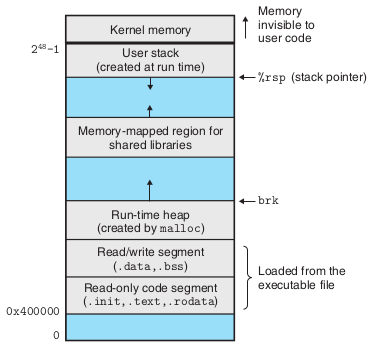
\includegraphics[width=\textwidth]{images/loaded_executable.png}

\end{minipage}



%%================
\WhatToReadSection
%%================
\begin{tabular}{@{}l@{}}
  \citeauthor[глава~7, стр.~634--660]{Bryant:2022:ru} \\
  \citeauthor[глава~7, стр.~571--592]{Tanenbaum:2007:ru}
\end{tabular}

%% !TEX encoding   = UTF8
% !TEX spellcheck = ru_RU
% !TEX root = ../seminars.tex

%%==============================
\chapter{Архитектура компьютера}
%%==============================

%%===============================
\section{Архитектура фон Неймана}
%%===============================
\noindent
\begin{minipage}{0.4\columnwidth}
  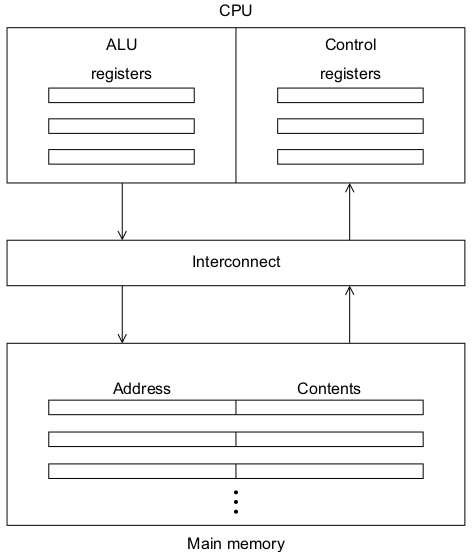
\includegraphics[width=\columnwidth]{images/von_neumann_architecture.png}
\end{minipage}\hfill
\begin{minipage}{0.5\columnwidth}
\parindent=2.5em
\textit{Центральный процессор} (ЦП), или \textenglish{central processor unit} (CPU), "--- это мозг компьютера. Его задача "--- выполнять программы, расположенные в~основной памяти. Он вызывает команды из~памяти, определяет их тип, а затем выполняет одну за~другой. Компоненты соединены \textit{шиной} (\textenglish{bus}), представляющей собой набор параллельно связанных проводов, по~которым передаются адреса, данные и сигналы управления. Шины могут быть внешними (связывающими процессор с~памятью и устройствами ввода--вывода) и внутренними.

Системы RISC (\textenglish{Reduced Instruction Set Computer}) и CISC (\textenglish{Complex Instruction Set Computer}).
\end{minipage}



%%========================================
\section{Процессы, многозадачность и нити}
%%========================================
\textit{Операционная система}~(ОС) "--- существенная часть программного обеспечения, задача которого управлять аппаратными и программными ресурсами компьютера.

Когда пользователь запускает программу, операционная система создаёт \textit{процесс} "--- копию программы, которая может быть выполнена. Он состоит из~нескольких элементов:
\begin{itemfeature}
  \item Код на~машинном языке.
  \item Блок памяти, которая будет включать исполняемый код, \textit{стек вызовов} (\textenglish{call stack}), динамически распределяемую память (кучу, \textenglish{heap}) и некоторые другие части.
  \item Дескрипторы ресурсов, которые операционная система выделяет для~процесса.
  \item Права доступа "--- информация, определяющая какие аппаратные и программные ресурсы доступны данному процессу.
  \item Информация о~состоянии: готов ли процесс к~выполнению или ожидает ресурс, содержимое регистров, распределение занимаемой памяти.
\end{itemfeature}

Большинство современных операционных систем \textit{многозадачные} (\textenglish{multitasking}). Это означает, что они обеспечивают поддержку одновременного выполнения нескольких программ (даже на~одном ядре). После того, как одна запущенная программа отработала небольшой интервал времени (несколько миллисекунд), называемый \textit{квантом} (\textenglish{time slice}), операционная система может запустить другую программу.

Если в~многозадачной ОС процесс ожидает ресурса, то он \textit{блокируется} (\textenglish{block}). Это означает, что его выполнение приостанавливается, и операционная система может запустить другой процесс. \textit{Нити} (\textenglish{threading}) исполнения обеспечивают механизм для~разделения программы на~более или менее независимые задачи так, что когда одна нить блокируется, другая может выполняться. Нить создаётся внутри процесса и разделяет большую часть его ресурсов. Два наиболее важных исключения "--- счётчик команд и стек вызовов. Поэтому создание и переключение между нитями происходит быстрее, чем между процессами.



%%======================================
\section{Модификации модели фон~Неймана}
%%======================================
\vspace{-1em}\begin{flushleft}
  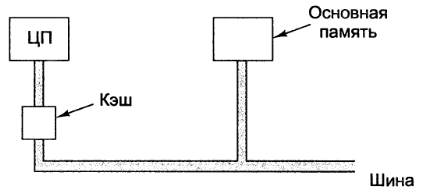
\includegraphics[width=0.45\columnwidth]{images/cache.png}\hfill%
  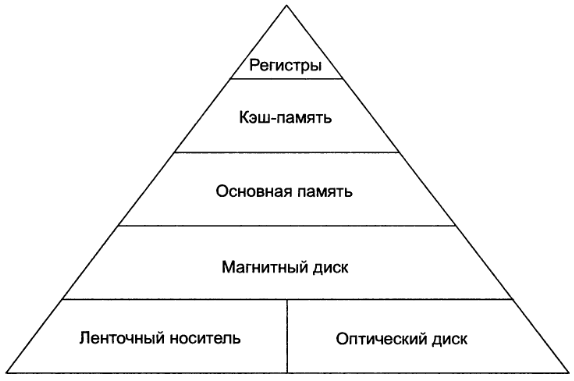
\includegraphics[width=0.45\columnwidth]{images/memory.png}
\end{flushleft}



%%================================
\subparagraph{Основы кэширования.}
%%================================
Кэш-память, или \textit{кэш}~(\textenglish{cache}), "--- набор блоков памяти, обращение к~которым может быть выполнено за~меньшее время, чем к~основной памяти.

С~появлением кэша, сразу возникает вопрос, какие данные и инструкции следует там хранить. В~основе универсальной стратегии лежит идея, что программа стремится использовать данные и инструкции, которые физически расположены рядом с~теми, что использовались недавно. Эту стратегию часто называют \emph{принципом локальности}. За~обращением по~некоторому адресу для~извлечения инструкции или данных в~следующий момент (\emph{временная} локальность) обычно происходит обращение к~соседнему адресу (\emph{пространственная} локальность). Ярким примером служит работа с~массивами.

Для~реализации принципа локальности на~практике система использует \emph{шину}, или соединительные провода, достаточно большой ширины. То есть при~обращении к~памяти в~действительности происходят операции с~блоками данных и инструкций, которые называют \emph{кэш-блоками} или \emph{строками кэша}.

Концептуально, зачастую удобно думать о~кэше ЦП, как о~единой структуре. Однако на~практике его обычно разделяют на~\emph{уровни}: первый уровень~(L1) самый маленький и самый быстрый, более высокие уровни~(L2, L3, \ldots) больше и медленнее.

Когда центральному процессору необходимо загрузить инструкции или данные, он просматривает кэш: в~начале проверяет первый уровень, затем второй и т.\,д. Если необходимая информация найдена, это называют \textit{кэш-попаданием} (\textenglish{cache hit}). А если нет, то это \textit{кэш-промах} (\textenglish{cache miss}), и процессор обращается к~основной памяти, что может приостановить выполнение текущей программы до~тех пор, пока не~будут получены данные.

Для~измерения эффективности вводят \emph{коэффициент кэш-попаданий}~\(h\) (\textenglish{hit ratio}), который показывает соотношение числа обращений к~кэш-памяти и общего числа всех обращений к~памяти, и \emph{коэффициент кэш-промахов} (\textenglish{miss ratio}), равный \(1 - h\).

Пусть~\(c\) "--- время доступа к~кэш-памяти, \(m\) "--- время доступа к~основной памяти. Тогда среднее время доступа:
\[
  t_\text{ave} = c + (1 - h)\,m.
\]
Если \(h \rightarrow 1\), то есть все обращения делаются только к~кэш-памяти, то время доступа стремится к~\(c\). С~другой стороны, если \(h \rightarrow 0\), то есть каждый раз нужно обращаться к~основной памяти, то время доступа стремится к~\(c + m\): сначала требуется время~\(c\) для~проверки кэш-памяти (в~данном случае безуспешной), а затем "--- время~\(m\) для~обращения к~основной памяти.

Когда ЦП пишет данные в~кэш, значение в~кэше и основной памяти становятся различными, или \textit{несогласованными} (\textenglish{inconsistent}). Существует два подхода устранить несогласованность. Немедленное обновление значения в~основной памяти называется \textit{сквозной записью} (\textenglish{write-through}). Этот подход обычно гораздо проще реализуется и, к~тому же, более надёжен, поскольку современная память при~ошибке может восстановить своё предыдущее состояние. К~сожалению, при~этом приходится передавать больше данных в~память, поэтому в~сложных проектах стремятся использовать альтернативный подход "--- \textit{отложенную запись} (\textenglish{write-back}). Обновлённые данные в~кэше помечаются как <<грязные>> (\textenglish{dirty}), и когда строка кэша заменяется новой строкой из~памяти, <<грязная>> строка записывается обратно в~память.



%%================================
\paragraph{Отображение кэш-памяти}
%%================================
на~основную память:
\begin{itemfeature}
  \item \textit{полностью ассоциативный} кэш: строка может быть помещена в~любую позицию;
  \item кэш \textit{прямого отображения}: строка связана с~фиксированной позицией определяемой, например, младшими битами адреса в~основной памяти;
  \item \textit{n-входовый ассоциативный} кэш являет собой промежуточный вариант.
\end{itemfeature}



%%=============================
\paragraph{Виртуальная память.}
%%=============================
Современные операционные системы поддерживают одновременную работу множества задач, которые вынуждены разделять ресурс памяти меж собой. Кроме того, необходимо защищать данные и инструкции каждого процесса от~возможного повреждения со~стороны других процессов.

\emph{Виртуальная память} (\textenglish{virtual memory}) разработана так, чтобы основная память могла быть использована как кэш для~вторичного хранилища (обычно в~дисковом пространстве). Она использует принцип пространственной и временной локальности, сохраняя в~основной памяти только активные части запущенных программ; те части, что простаивают, хранятся в~блоке вторичного хранилища, называемом \textit{файлом подкачки} (\textenglish{swap space}). Подобно кэшу, виртуальная память оперирует с~блоками данных и инструкций. Эти блоки обычно называют \emph{страницами} (\textenglish{pages}). Поскольку доступ ко~вторичному хранилищу может быть в~сотни тысяч раз медленнее, чем к~основной памяти, страницы делают относительно большими "--- большинство систем имеют фиксированный размер страниц, который на~данный момент лежит в~диапазоне от~4 до~16\,Кб.

При~компиляции программы используются виртуальные адреса. Когда программа запускается, создаётся \emph{таблица страниц} (\textenglish{page table}) для~отображения виртуальных страниц на~физические адреса. Обычно создание таблиц осуществляет операционная система, что позволяет гарантировать, что участки памяти, используемые одним процессом, не~пересекается с~памятью других процессов.

Недостаток использования таблиц в~удвоении времени доступа к~основной памяти (обращение к~таблице плюс обращение в~память по~целевому физическому адресу). Для~решения этой проблемы процессоры содержат специальный кэш для~преобразования адресов, называемый \emph{буфером быстрого преобразования} (\textenglish{translation-lookaside buffer, TLB}).

Вследствие медленной работы диска виртуальная память всегда использует отложенную запись, если страница была изменена в~процессе работы программы. А управление таблицой страниц и обращением к~диску можно поручить операционной системе (совместно с~аппаратным обеспечением).



%%=====================================================
\paragraph{Параллелизм выполнения на~уровне инструкций}
%%=====================================================
позволяет улучшить производительность процессора за~счёт разделения на~компоненты, или \emph{функциональные блоки} (\textenglish{functional units}), одновременно выполняющие инструкции.

Существует два основных подхода:
\begin{itemfeature}
  \item \emph{конвейер} (\textenglish{pipeline}), принцип работы схож с~заводским конвейером;
  \item \emph{суперскалярная архитектура} (\textenglish{superscalar architecture}), один конвейер с~большим количеством функциональных блоков.
\end{itemfeature}

\begin{center}
  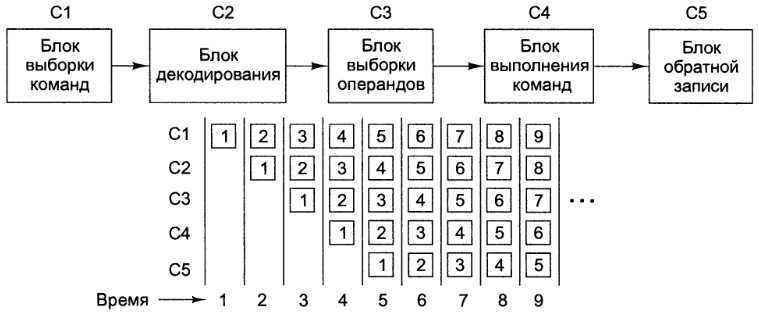
\includegraphics[width=0.7\columnwidth]{images/pipeline.png}
\end{center}



%%=============================================
\paragraph{Многонитевое аппаратное обеспечение}
%%=============================================
предоставляет средства для~продолжения выполнения полезной работы, когда задача, выполняющаяся в~данный момент, была приостановлена, например, в~ожидании загрузки данных из~памяти. В~этот момент, возможно, имеет смысл просто запустить другую нить. Конечно, для~этого система должна поддерживать очень быстрое переключение между нитями.



%%===========================================
\section{Параллельное аппаратное обеспечение}
%%===========================================
Суперскалярную архитектуру и конвейер также можно рассматривать как параллельное аппаратное обеспечение, поскольку функциональные блоки дублируются. Однако, эта форма параллелизма обычно не~видна программисту, и её можно рассматривать как расширение исходной модели фон~Неймана. Под~\emph{параллельным обеспечением} будем понимать обеспечение, которое требует от~программиста изменений в~исходном коде.



%%=======================
\paragraph{SIMD системы.}
%%=======================
\textenglish{Single Instruction-stream Multiple Data-stream}:
\begin{itemfeature}
  \item \emph{векторные процессоры} (\textenglish{vector processors});
  \item \emph{графические процессоры} (\textenglish{graphics processing units, GPU})
\end{itemfeature}



%%=======================
\paragraph{MIMD системы.}
%%=======================
\textenglish{Multiple Instruction-stream Multiple Data-stream}:

\medskip\noindent
\begin{minipage}[c]{0.5\textwidth}
\parindent=2.5em

\begin{itemfeature}
  \item \emph{системы с~общей памятью} (\textenglish{shared-memory systems}), используют один или более многоядерных процессоров, связанных с~единой памятью. Выделяют системы с~\emph{однородным доступов к~памяти} (\textenglish{uniform memory access, UMA}) и \emph{неоднородным доступом к~памяти} (\textenglish{nonuniform memory access, NUMA});
\end{itemfeature}

\end{minipage}\hfill\begin{minipage}{0.45\textwidth}

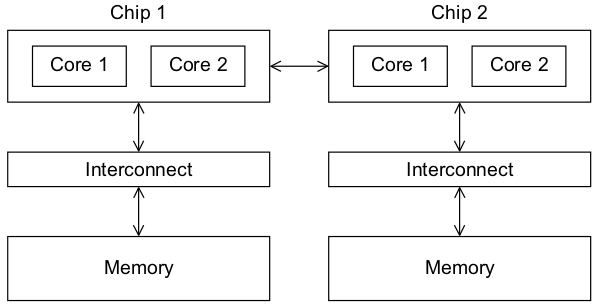
\includegraphics[width=\columnwidth]{images/numa_multicore_system.png}

\end{minipage}

\begin{itemfeature}
  \item \emph{системы с~распределённой памятью} (\textenglish{distributed-memory systems}). Обычно \emph{узлами} (\textenglish{nodes}) таких систем являются системы с~общей памятью, поэтому их иногда называют \emph{гибридными} (\textenglish{hybrid systems}). \emph{Глобальная сеть} (\textenglish{grid}) обеспечивает инфраструктуру, необходимую для~объединения больших сетей географически распределённых компьютеров в~одно целое. В~общем, такие системы будут \emph{гетерогенными} (\textenglish{heterogeneous}), то есть индивидуальные узлы могут иметь разную архитектуру.
\end{itemfeature}



%%===============
\ExercisesSection
%%===============
Рассмотрим влияние кэширования на~производительность программы. Для~этого создадим структуру данных, которая хранит целочисленный идентификатор и массив символов фиксированного размера.

\cppfile[firstline=13, lastline=19]{projects/sem14/cache.cpp}



%%============================
\paragraph{Тестовая оснастка.}
%%============================
Напишем функцию, которая создаёт тестовый массив заданного размера, заполняя поле \code{id} элементов псевдослучайными значениями в~диапазоне от~\code{0} до~\code{high}.

\cppfile[firstline=22, lastline=36]{projects/sem14/cache.cpp}

\noindent Здесь используются возможности стандартной библиотеки \code{<random>}. При~желании, можно выбрать другое распределение, отличное от~равномерного. Обратим внимание на~пустые скобки при~указании шаблонного типа. Объявление класса выглядит примерно так:

\begin{minted}[linenos=false, fontsize=\small]{c++}
template<class IntType = int>
class uniform_int_distribution;
\end{minted}

\noindent Видно, что параметр по~умолчанию "--- тип \code{int}. Именно поэтому мы можем его не~указывать явно. А угловые скобки говорят о~том, что это шаблон.

Напишем тестовую функцию, которая запускает два различных варианта упорядочивания элементов в~массиве заданного размера и измеряет время выполнения каждого алгоритма. Добавим проверку, что оба варианта приводят к~одинаковому порядку. В~качестве таймера можно использовать класс-обёртку \code{Timer}, описание которого приведём ниже.

\cppfile[firstline=80, lastline=101]{projects/sem14/cache.cpp}

Функцию \code{main()} нашей тестовой программы можно записать следующим образом:

\cppfile[firstline=104, lastline=104]{projects/sem14/cache.cpp}
\cppfile[firstline=106, lastline=115]{projects/sem14/cache.cpp}



%%===============================
\paragraph{Класс \texttt{Timer}.}
%%===============================
Это небольшой класс-обёртка, использующий стандартную библиотеку \code{<chrono>}. Его реализация проста и очевидна, не~требует дополнительных комментариев. Код следует разместить в~файле \code{timer.h} и подключить к~коду остальной тестовой оснастки.

\cppfile[firstline=7, lastline=30]{projects/sem14/timer.h}

Теперь рассмотрим первый вариант сортировки. Упорядочивать будем по~полю \code{id}. Положим, что элементы массива достаточно велики, чтобы пренебречь временем копирования при~обменах. Для~решения этой проблемы создадим массив указателей и упорядочим его. (В~случае необходимости легко получить новый, упорядоченный, массив исходных элементов, используя указатели.)

\cppfile[firstline=39, lastline=51]{projects/sem14/cache.cpp}

Второй вариант сделаем чуть хитрее. Добавим вспомогательный массив пар \code{(указатель, id)} и выполним упорядочивание без~косвенного доступа к~исходным элементам.

\cppfile[firstline=54, lastline=77]{projects/sem14/cache.cpp}

Проведите серию запусков программы и постройте несколько графиков подобных тем, что приведены на~рисунке~\ref{fig:caching}.

\begin{figure}[h]
  {\centering
    \hfill
    \subbottom[в~зависимости от~количества элементов\label{fig:caching:a}]{%
      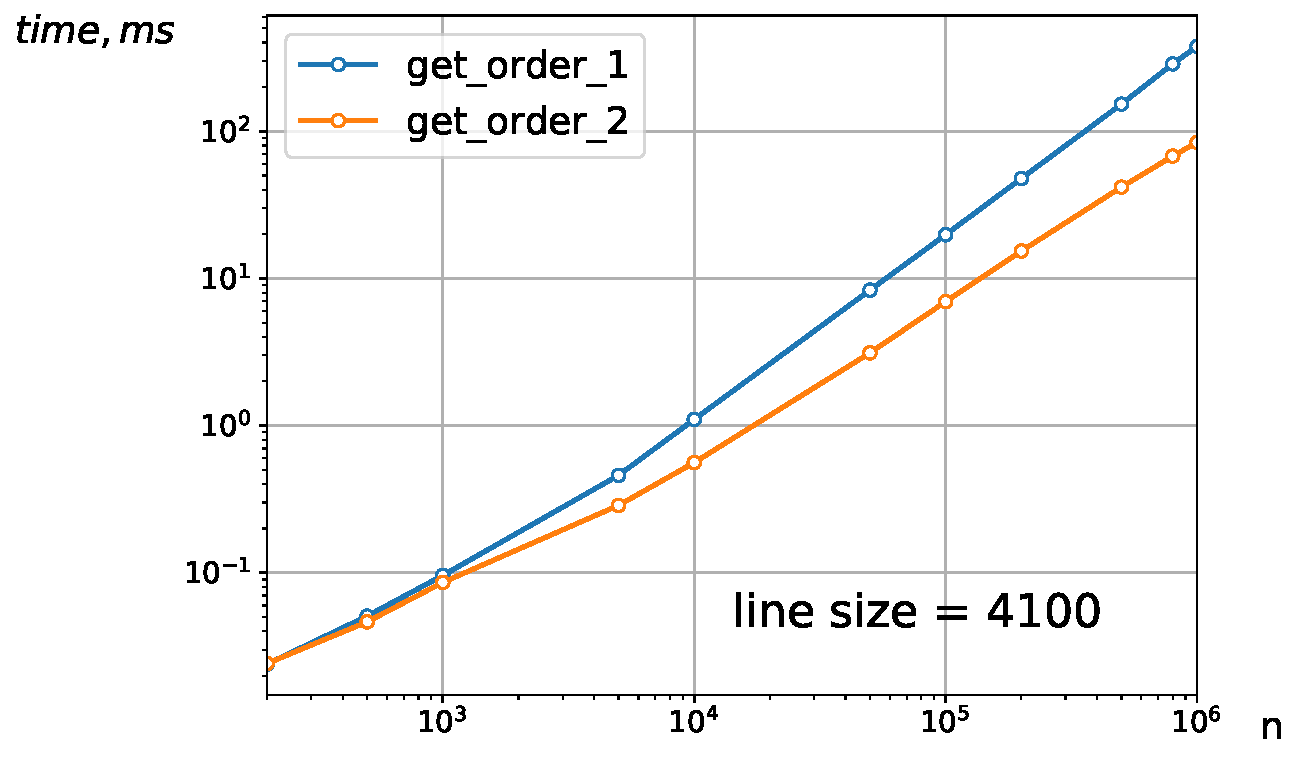
\includegraphics[width=0.45\columnwidth]{images/cache_impact_by_n.pdf}}
    \hfill
    \subbottom[в~зависимости от~размера самого элемента\label{fig:caching:b}]{%
      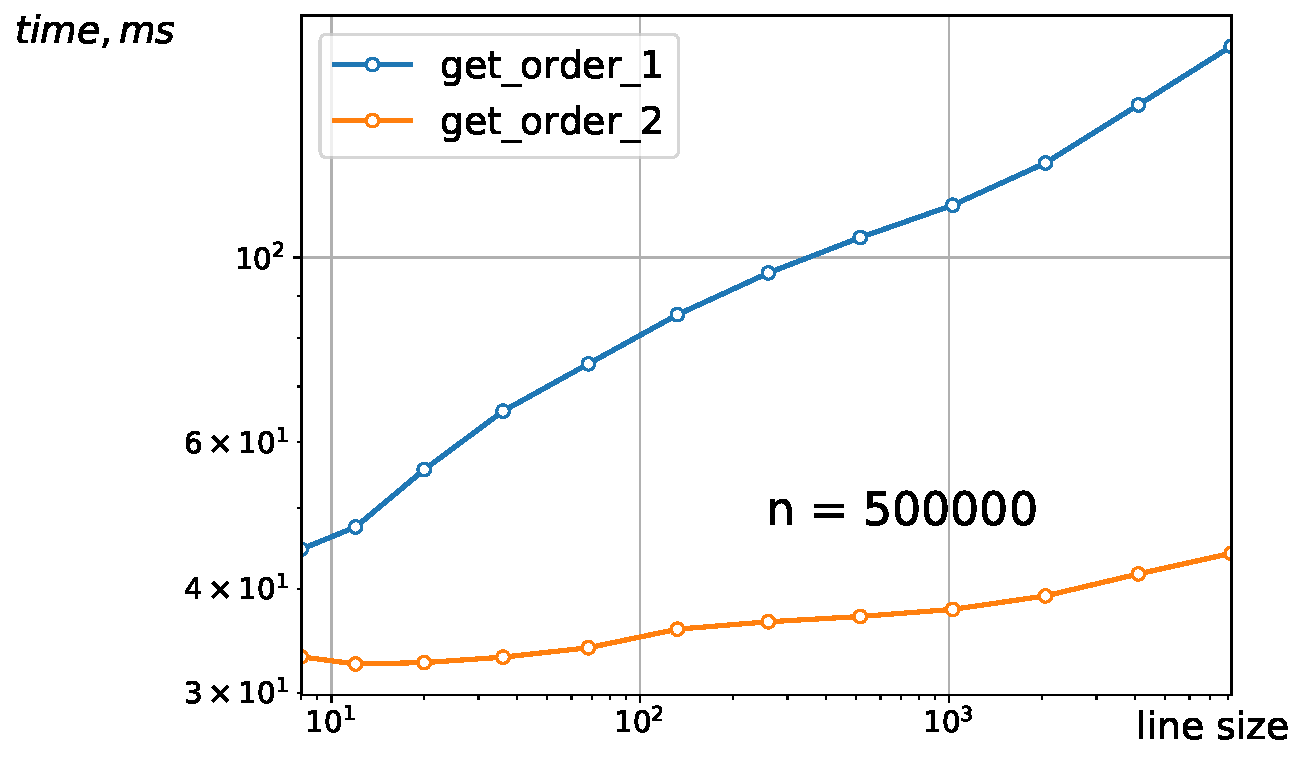
\includegraphics[width=0.45\columnwidth]{images/cache_impact_by_line_size.pdf}}
    \hfill
    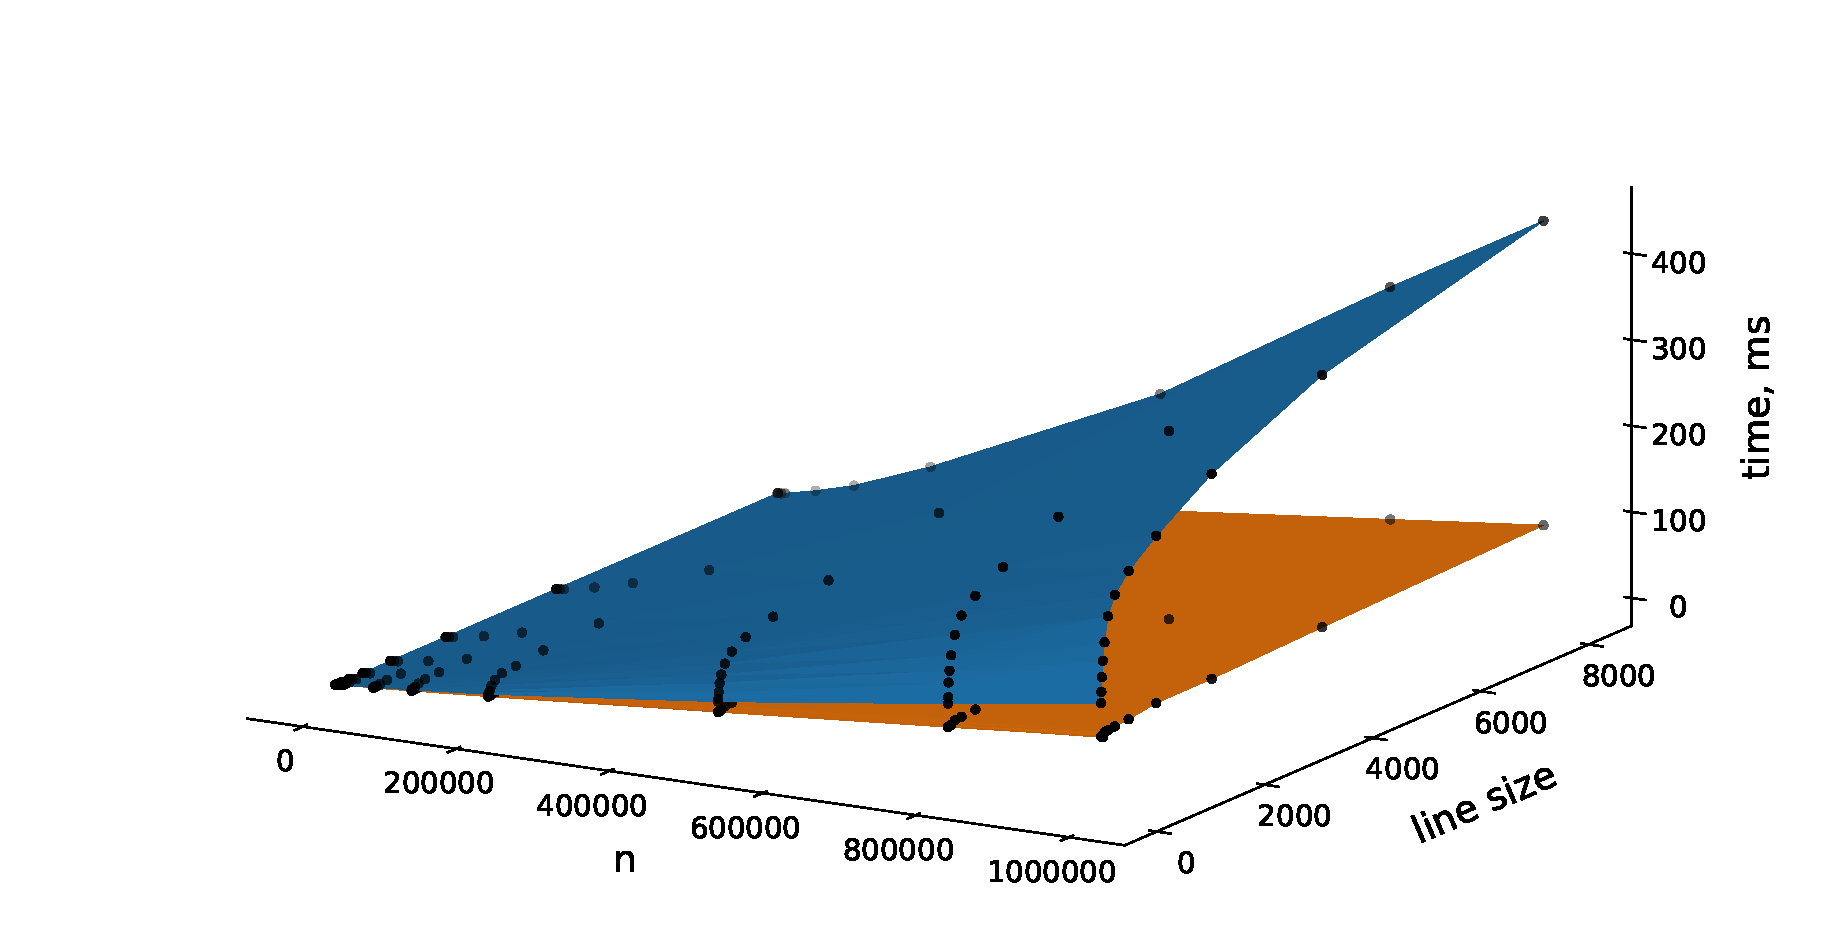
\includegraphics[width=0.7\columnwidth]{images/cache_impact.pdf}

  }
  \caption{Влияние кэширования на~производительность программы.}
  \label{fig:caching}
\end{figure}

Объясните полученное поведение кривых. Используйте знания об~устройстве и работе кэша, изложенные выше.



%%================
\WhatToReadSection
%%================
\begin{tabular}{@{}l@{}}
  \citeauthor[глава~3, стр.~390--398]{Harris:2015:ru} \\
  \citeauthor[глава~7, стр.~1091--1131; глава~8, стр.~1163--1240]{Harris:2015:ru} \\
  \citeauthor[глава~2, стр.~15--46]{Pacheco:2011:en}
\end{tabular}



\backmatter
%%=========
% !TEX encoding   = UTF8
% !TEX spellcheck = en_US

\clearpage

%\hypersetup{ urlcolor=black }

%\providecommand*{\BibDash}{}
\urlstyle{rm}
\ifdefmacro{\microtypesetup}{\microtypesetup{protrusion=false}}{}
\printbibliography[heading=bibintoc]
\ifdefmacro{\microtypesetup}{\microtypesetup{protrusion=true}}{}
\urlstyle{tt}

%\hypersetup{ urlcolor={urlcolor} }



\appendix
%========
% !TEX encoding   = UTF8
% !TEX spellcheck = ru_RU
% !TEX root = seminars.tex

%%==================
\chapter{Приложение}
%%==================
%%===========================================
\section{Установка и настройка рабочей среды}\label{sect:workEnv}
%%===========================================

\todo{Добавить материал}


\end{document}
